\documentclass[twoside]{book}

% Packages required by doxygen
\usepackage{calc}
\usepackage{doxygen}
\usepackage{graphicx}
\usepackage[utf8]{inputenc}
\usepackage{makeidx}
\usepackage{multicol}
\usepackage{multirow}
\usepackage{textcomp}
\usepackage[table]{xcolor}

% NLS support packages
\usepackage[french]{babel}

% Font selection
\usepackage[T1]{fontenc}
\usepackage{mathptmx}
\usepackage[scaled=.90]{helvet}
\usepackage{courier}
\usepackage{amssymb}
\usepackage{sectsty}
\renewcommand{\familydefault}{\sfdefault}
\allsectionsfont{%
  \fontseries{bc}\selectfont%
  \color{darkgray}%
}
\renewcommand{\DoxyLabelFont}{%
  \fontseries{bc}\selectfont%
  \color{darkgray}%
}

% Page & text layout
\usepackage{geometry}
\geometry{%
  a4paper,%
  top=2.5cm,%
  bottom=2.5cm,%
  left=2.5cm,%
  right=2.5cm%
}
\tolerance=750
\hfuzz=15pt
\hbadness=750
\setlength{\emergencystretch}{15pt}
\setlength{\parindent}{0cm}
\setlength{\parskip}{0.2cm}
\makeatletter
\renewcommand{\paragraph}{%
  \@startsection{paragraph}{4}{0ex}{-1.0ex}{1.0ex}{%
    \normalfont\normalsize\bfseries\SS@parafont%
  }%
}
\renewcommand{\subparagraph}{%
  \@startsection{subparagraph}{5}{0ex}{-1.0ex}{1.0ex}{%
    \normalfont\normalsize\bfseries\SS@subparafont%
  }%
}
\makeatother

% Headers & footers
\usepackage{fancyhdr}
\pagestyle{fancyplain}
\fancyhead[LE]{\fancyplain{}{\bfseries\thepage}}
\fancyhead[CE]{\fancyplain{}{}}
\fancyhead[RE]{\fancyplain{}{\bfseries\leftmark}}
\fancyhead[LO]{\fancyplain{}{\bfseries\rightmark}}
\fancyhead[CO]{\fancyplain{}{}}
\fancyhead[RO]{\fancyplain{}{\bfseries\thepage}}
\fancyfoot[LE]{\fancyplain{}{}}
\fancyfoot[CE]{\fancyplain{}{}}
\fancyfoot[RE]{\fancyplain{}{\bfseries\scriptsize Généré le Jeudi 6 Mars 2014 16\-:19\-:38 pour Module Bench\-Mark par Doxygen }}
\fancyfoot[LO]{\fancyplain{}{\bfseries\scriptsize Généré le Jeudi 6 Mars 2014 16\-:19\-:38 pour Module Bench\-Mark par Doxygen }}
\fancyfoot[CO]{\fancyplain{}{}}
\fancyfoot[RO]{\fancyplain{}{}}
\renewcommand{\footrulewidth}{0.4pt}
\renewcommand{\chaptermark}[1]{%
  \markboth{#1}{}%
}
\renewcommand{\sectionmark}[1]{%
  \markright{\thesection\ #1}%
}

% Indices & bibliography
\usepackage{natbib}
\usepackage[titles]{tocloft}
\setcounter{tocdepth}{3}
\setcounter{secnumdepth}{5}
\makeindex

% Hyperlinks (required, but should be loaded last)
\usepackage{ifpdf}
\ifpdf
  \usepackage[pdftex,pagebackref=true]{hyperref}
\else
  \usepackage[ps2pdf,pagebackref=true]{hyperref}
\fi
\hypersetup{%
  colorlinks=true,%
  linkcolor=blue,%
  citecolor=blue,%
  unicode%
}

% Custom commands
\newcommand{\clearemptydoublepage}{%
  \newpage{\pagestyle{empty}\cleardoublepage}%
}


%===== C O N T E N T S =====

\begin{document}

% Titlepage & ToC
\hypersetup{pageanchor=false}
\pagenumbering{roman}
\begin{titlepage}
\vspace*{7cm}
\begin{center}%
{\Large Module Bench\-Mark \\[1ex]\large 1 }\\
\vspace*{1cm}
{\large Généré par Doxygen 1.8.6}\\
\vspace*{0.5cm}
{\small Jeudi 6 Mars 2014 16:19:38}\\
\end{center}
\end{titlepage}
\clearemptydoublepage
\tableofcontents
\clearemptydoublepage
\pagenumbering{arabic}
\hypersetup{pageanchor=true}

%--- Begin generated contents ---
\chapter{Module Bench\-Mark}
\label{index}\hypertarget{index}{}Ce module a pour but d'écrire les erreurs dans un fichier \char`\"{}log.\-txt\char`\"{} afin d'en garder une trace si on veut les consulter.

{\bfseries Exemple de B\-O\-N\-N\-E utilisation du module \-: } \begin{DoxyVerb}  Log.error("l'erreur");
  Log.reset();\end{DoxyVerb}
 
\chapter{Index des espaces de nommage}
\section{Paquetages}
Liste des paquetages avec une brève description (si disponible) \-:\begin{DoxyCompactList}
\item\contentsline{section}{\hyperlink{namespacecom}{com} }{\pageref{d8/dee/namespacecom}}{}
\item\contentsline{section}{\hyperlink{namespacecom_1_1error__manager}{com.\-error\-\_\-manager} }{\pageref{d9/df7/namespacecom_1_1error__manager}}{}
\item\contentsline{section}{\hyperlink{namespacecom_1_1error__manager_1_1test}{com.\-error\-\_\-manager.\-test} }{\pageref{d5/d4b/namespacecom_1_1error__manager_1_1test}}{}
\end{DoxyCompactList}

\chapter{Index hiérarchique}
\section{Hiérarchie des classes}
Cette liste d'héritage est classée approximativement par ordre alphabétique \-:\begin{DoxyCompactList}
\item Applet\begin{DoxyCompactList}
\item \contentsline{section}{jnt.\-Bench.\-Applet}{\pageref{d7/ddf/classjnt_1_1Bench_1_1Applet}}{}
\end{DoxyCompactList}
\item \contentsline{section}{jnt.\-Bench\-Mark}{\pageref{d3/d2c/classjnt_1_1BenchMark}}{}
\item \contentsline{section}{jnt.\-Bench\-Mark\-Result}{\pageref{df/d04/classjnt_1_1BenchMarkResult}}{}
\item \contentsline{section}{jnt.\-Bench\-Mark\-Result\-Event}{\pageref{d3/dcf/interfacejnt_1_1BenchMarkResultEvent}}{}
\item \contentsline{section}{jnt.\-scimark2.\-Constants}{\pageref{d5/d9d/classjnt_1_1scimark2_1_1Constants}}{}
\item \contentsline{section}{jnt.\-scimark2.\-F\-F\-T}{\pageref{d2/d87/classjnt_1_1scimark2_1_1FFT}}{}
\item \contentsline{section}{jnt.\-Bench\-Mark\-Result.\-F\-F\-T}{\pageref{dd/d0a/classjnt_1_1BenchMarkResult_1_1FFT}}{}
\item \contentsline{section}{jnt.\-Bench.\-Formatter}{\pageref{d2/dcd/classjnt_1_1Bench_1_1Formatter}}{}
\item Frame\begin{DoxyCompactList}
\item \contentsline{section}{jnt.\-Bench.\-Submit\-Dialog}{\pageref{d0/da7/classjnt_1_1Bench_1_1SubmitDialog}}{}
\end{DoxyCompactList}
\item \contentsline{section}{jnt.\-Bench.\-H\-T\-T\-P\-Post}{\pageref{de/df0/classjnt_1_1Bench_1_1HTTPPost}}{}
\item \contentsline{section}{jnt.\-scimark2.\-Jacobi}{\pageref{d9/d30/classjnt_1_1scimark2_1_1Jacobi}}{}
\item \contentsline{section}{jnt.\-scimark2.\-kernel}{\pageref{d0/d13/classjnt_1_1scimark2_1_1kernel}}{}
\item \contentsline{section}{jnt.\-Bench\-Mark\-Result.\-L\-U}{\pageref{d6/dfb/classjnt_1_1BenchMarkResult_1_1LU}}{}
\item \contentsline{section}{jnt.\-scimark2.\-L\-U}{\pageref{d5/d6c/classjnt_1_1scimark2_1_1LU}}{}
\item \contentsline{section}{jnt.\-Bench\-Mark\-Result.\-Monte\-Carlo}{\pageref{d0/d37/classjnt_1_1BenchMarkResult_1_1MonteCarlo}}{}
\item \contentsline{section}{jnt.\-scimark2.\-Monte\-Carlo}{\pageref{dd/db2/classjnt_1_1scimark2_1_1MonteCarlo}}{}
\item \contentsline{section}{jnt.\-scimark2.\-Random}{\pageref{d0/d74/classjnt_1_1scimark2_1_1Random}}{}
\item Runnable\begin{DoxyCompactList}
\item \contentsline{section}{jnt.\-Bench.\-Bench}{\pageref{d1/d59/classjnt_1_1Bench_1_1Bench}}{}
\end{DoxyCompactList}
\item \contentsline{section}{jnt.\-Bench.\-Send\-Mail}{\pageref{d3/d4e/classjnt_1_1Bench_1_1SendMail}}{}
\item \contentsline{section}{jnt.\-Bench\-Mark\-Result.\-S\-O\-R}{\pageref{d8/dcd/classjnt_1_1BenchMarkResult_1_1SOR}}{}
\item \contentsline{section}{jnt.\-scimark2.\-S\-O\-R}{\pageref{d8/d38/classjnt_1_1scimark2_1_1SOR}}{}
\item \contentsline{section}{jnt.\-scimark2.\-Sparse\-Comp\-Row}{\pageref{db/dbd/classjnt_1_1scimark2_1_1SparseCompRow}}{}
\item \contentsline{section}{jnt.\-Bench\-Mark\-Result.\-Sparse\-Matmult}{\pageref{d5/ded/classjnt_1_1BenchMarkResult_1_1SparseMatmult}}{}
\item \contentsline{section}{jnt.\-scimark2.\-Stopwatch}{\pageref{d2/d17/classjnt_1_1scimark2_1_1Stopwatch}}{}
\item \contentsline{section}{jnt.\-Bench.\-Stopwatch}{\pageref{d9/d48/classjnt_1_1Bench_1_1Stopwatch}}{}
\item \contentsline{section}{jnt.\-Bench.\-Target}{\pageref{de/d37/interfacejnt_1_1Bench_1_1Target}}{}
\begin{DoxyCompactList}
\item \contentsline{section}{jnt.\-scimark2.\-applet}{\pageref{dd/dfe/classjnt_1_1scimark2_1_1applet}}{}
\end{DoxyCompactList}
\item Canvas\begin{DoxyCompactList}
\item \contentsline{section}{jnt.\-Bench.\-Plotter}{\pageref{da/d70/classjnt_1_1Bench_1_1Plotter}}{}
\end{DoxyCompactList}
\end{DoxyCompactList}

\chapter{Index des classes}
\section{Liste des classes}
Liste des classes, structures, unions et interfaces avec une brève description \-:\begin{DoxyCompactList}
\item\contentsline{section}{\hyperlink{classjnt_1_1Bench_1_1Applet}{jnt.\-Bench.\-Applet} }{\pageref{d7/ddf/classjnt_1_1Bench_1_1Applet}}{}
\item\contentsline{section}{\hyperlink{classjnt_1_1scimark2_1_1applet}{jnt.\-scimark2.\-applet} }{\pageref{dd/dfe/classjnt_1_1scimark2_1_1applet}}{}
\item\contentsline{section}{\hyperlink{classjnt_1_1Bench_1_1Bench}{jnt.\-Bench.\-Bench} }{\pageref{d1/d59/classjnt_1_1Bench_1_1Bench}}{}
\item\contentsline{section}{\hyperlink{classjnt_1_1BenchMark}{jnt.\-Bench\-Mark} }{\pageref{d3/d2c/classjnt_1_1BenchMark}}{}
\item\contentsline{section}{\hyperlink{classjnt_1_1BenchMarkResult}{jnt.\-Bench\-Mark\-Result} }{\pageref{df/d04/classjnt_1_1BenchMarkResult}}{}
\item\contentsline{section}{\hyperlink{interfacejnt_1_1BenchMarkResultEvent}{jnt.\-Bench\-Mark\-Result\-Event} }{\pageref{d3/dcf/interfacejnt_1_1BenchMarkResultEvent}}{}
\item\contentsline{section}{\hyperlink{classjnt_1_1scimark2_1_1Constants}{jnt.\-scimark2.\-Constants} }{\pageref{d5/d9d/classjnt_1_1scimark2_1_1Constants}}{}
\item\contentsline{section}{\hyperlink{classjnt_1_1scimark2_1_1FFT}{jnt.\-scimark2.\-F\-F\-T} }{\pageref{d2/d87/classjnt_1_1scimark2_1_1FFT}}{}
\item\contentsline{section}{\hyperlink{classjnt_1_1BenchMarkResult_1_1FFT}{jnt.\-Bench\-Mark\-Result.\-F\-F\-T} }{\pageref{dd/d0a/classjnt_1_1BenchMarkResult_1_1FFT}}{}
\item\contentsline{section}{\hyperlink{classjnt_1_1Bench_1_1Formatter}{jnt.\-Bench.\-Formatter} }{\pageref{d2/dcd/classjnt_1_1Bench_1_1Formatter}}{}
\item\contentsline{section}{\hyperlink{classjnt_1_1Bench_1_1HTTPPost}{jnt.\-Bench.\-H\-T\-T\-P\-Post} }{\pageref{de/df0/classjnt_1_1Bench_1_1HTTPPost}}{}
\item\contentsline{section}{\hyperlink{classjnt_1_1scimark2_1_1Jacobi}{jnt.\-scimark2.\-Jacobi} }{\pageref{d9/d30/classjnt_1_1scimark2_1_1Jacobi}}{}
\item\contentsline{section}{\hyperlink{classjnt_1_1scimark2_1_1kernel}{jnt.\-scimark2.\-kernel} }{\pageref{d0/d13/classjnt_1_1scimark2_1_1kernel}}{}
\item\contentsline{section}{\hyperlink{classjnt_1_1BenchMarkResult_1_1LU}{jnt.\-Bench\-Mark\-Result.\-L\-U} }{\pageref{d6/dfb/classjnt_1_1BenchMarkResult_1_1LU}}{}
\item\contentsline{section}{\hyperlink{classjnt_1_1scimark2_1_1LU}{jnt.\-scimark2.\-L\-U} }{\pageref{d5/d6c/classjnt_1_1scimark2_1_1LU}}{}
\item\contentsline{section}{\hyperlink{classjnt_1_1BenchMarkResult_1_1MonteCarlo}{jnt.\-Bench\-Mark\-Result.\-Monte\-Carlo} }{\pageref{d0/d37/classjnt_1_1BenchMarkResult_1_1MonteCarlo}}{}
\item\contentsline{section}{\hyperlink{classjnt_1_1scimark2_1_1MonteCarlo}{jnt.\-scimark2.\-Monte\-Carlo} }{\pageref{dd/db2/classjnt_1_1scimark2_1_1MonteCarlo}}{}
\item\contentsline{section}{\hyperlink{classjnt_1_1Bench_1_1Plotter}{jnt.\-Bench.\-Plotter} }{\pageref{da/d70/classjnt_1_1Bench_1_1Plotter}}{}
\item\contentsline{section}{\hyperlink{classjnt_1_1scimark2_1_1Random}{jnt.\-scimark2.\-Random} }{\pageref{d0/d74/classjnt_1_1scimark2_1_1Random}}{}
\item\contentsline{section}{\hyperlink{classjnt_1_1Bench_1_1SendMail}{jnt.\-Bench.\-Send\-Mail} }{\pageref{d3/d4e/classjnt_1_1Bench_1_1SendMail}}{}
\item\contentsline{section}{\hyperlink{classjnt_1_1BenchMarkResult_1_1SOR}{jnt.\-Bench\-Mark\-Result.\-S\-O\-R} }{\pageref{d8/dcd/classjnt_1_1BenchMarkResult_1_1SOR}}{}
\item\contentsline{section}{\hyperlink{classjnt_1_1scimark2_1_1SOR}{jnt.\-scimark2.\-S\-O\-R} }{\pageref{d8/d38/classjnt_1_1scimark2_1_1SOR}}{}
\item\contentsline{section}{\hyperlink{classjnt_1_1scimark2_1_1SparseCompRow}{jnt.\-scimark2.\-Sparse\-Comp\-Row} }{\pageref{db/dbd/classjnt_1_1scimark2_1_1SparseCompRow}}{}
\item\contentsline{section}{\hyperlink{classjnt_1_1BenchMarkResult_1_1SparseMatmult}{jnt.\-Bench\-Mark\-Result.\-Sparse\-Matmult} }{\pageref{d5/ded/classjnt_1_1BenchMarkResult_1_1SparseMatmult}}{}
\item\contentsline{section}{\hyperlink{classjnt_1_1scimark2_1_1Stopwatch}{jnt.\-scimark2.\-Stopwatch} }{\pageref{d2/d17/classjnt_1_1scimark2_1_1Stopwatch}}{}
\item\contentsline{section}{\hyperlink{classjnt_1_1Bench_1_1Stopwatch}{jnt.\-Bench.\-Stopwatch} }{\pageref{d9/d48/classjnt_1_1Bench_1_1Stopwatch}}{}
\item\contentsline{section}{\hyperlink{classjnt_1_1Bench_1_1SubmitDialog}{jnt.\-Bench.\-Submit\-Dialog} }{\pageref{d0/da7/classjnt_1_1Bench_1_1SubmitDialog}}{}
\item\contentsline{section}{\hyperlink{interfacejnt_1_1Bench_1_1Target}{jnt.\-Bench.\-Target} }{\pageref{de/d37/interfacejnt_1_1Bench_1_1Target}}{}
\end{DoxyCompactList}

\chapter{Index des fichiers}
\section{Liste des fichiers}
Liste de tous les fichiers avec une brève description \-:\begin{DoxyCompactList}
\item\contentsline{section}{\hyperlink{AllTests_8java}{All\-Tests.\-java} }{\pageref{d4/d12/AllTests_8java}}{}
\item\contentsline{section}{\hyperlink{Log_8java}{Log.\-java} }{\pageref{d4/d3d/Log_8java}}{}
\item\contentsline{section}{\hyperlink{LogTest_8java}{Log\-Test.\-java} }{\pageref{d2/d02/LogTest_8java}}{}
\end{DoxyCompactList}

\chapter{Documentation des espaces de nommage}
\hypertarget{namespacejnt}{\section{Paquetage jnt}
\label{namespacejnt}\index{jnt@{jnt}}
}
\subsection*{Paquetages}
\begin{DoxyCompactItemize}
\item 
package \hyperlink{namespacejnt_1_1Bench}{Bench}
\item 
package \hyperlink{namespacejnt_1_1scimark2}{scimark2}
\end{DoxyCompactItemize}
\subsection*{Classes}
\begin{DoxyCompactItemize}
\item 
class \hyperlink{classjnt_1_1BenchMark}{Bench\-Mark}
\item 
class \hyperlink{classjnt_1_1BenchMarkResult}{Bench\-Mark\-Result}
\item 
interface \hyperlink{interfacejnt_1_1BenchMarkResultEvent}{Bench\-Mark\-Result\-Event}
\end{DoxyCompactItemize}

\hypertarget{namespacejnt_1_1Bench}{\section{Paquetage jnt.\-Bench}
\label{namespacejnt_1_1Bench}\index{jnt.\-Bench@{jnt.\-Bench}}
}
\subsection*{Classes}
\begin{DoxyCompactItemize}
\item 
class \hyperlink{classjnt_1_1Bench_1_1Applet}{Applet}
\item 
class {\bfseries Applet\-Frame}
\item 
class \hyperlink{classjnt_1_1Bench_1_1Bench}{Bench}
\item 
class {\bfseries Segment}
\item 
class {\bfseries Entry}
\item 
class \hyperlink{classjnt_1_1Bench_1_1Formatter}{Formatter}
\item 
class \hyperlink{classjnt_1_1Bench_1_1HTTPPost}{H\-T\-T\-P\-Post}
\item 
class \hyperlink{classjnt_1_1Bench_1_1Plotter}{Plotter}
\item 
class \hyperlink{classjnt_1_1Bench_1_1SendMail}{Send\-Mail}
\item 
class \hyperlink{classjnt_1_1Bench_1_1Stopwatch}{Stopwatch}
\item 
class \hyperlink{classjnt_1_1Bench_1_1SubmitDialog}{Submit\-Dialog}
\item 
interface \hyperlink{interfacejnt_1_1Bench_1_1Target}{Target}
\end{DoxyCompactItemize}

\hypertarget{namespacejnt_1_1scimark2}{\section{Paquetage jnt.\-scimark2}
\label{namespacejnt_1_1scimark2}\index{jnt.\-scimark2@{jnt.\-scimark2}}
}
\subsection*{Classes}
\begin{DoxyCompactItemize}
\item 
class \hyperlink{classjnt_1_1scimark2_1_1applet}{applet}
\item 
class \hyperlink{classjnt_1_1scimark2_1_1Constants}{Constants}
\item 
class \hyperlink{classjnt_1_1scimark2_1_1FFT}{F\-F\-T}
\item 
class \hyperlink{classjnt_1_1scimark2_1_1Jacobi}{Jacobi}
\item 
class \hyperlink{classjnt_1_1scimark2_1_1kernel}{kernel}
\item 
class \hyperlink{classjnt_1_1scimark2_1_1LU}{L\-U}
\item 
class \hyperlink{classjnt_1_1scimark2_1_1MonteCarlo}{Monte\-Carlo}
\item 
class \hyperlink{classjnt_1_1scimark2_1_1Random}{Random}
\item 
class \hyperlink{classjnt_1_1scimark2_1_1SOR}{S\-O\-R}
\item 
class \hyperlink{classjnt_1_1scimark2_1_1SparseCompRow}{Sparse\-Comp\-Row}
\item 
class \hyperlink{classjnt_1_1scimark2_1_1Stopwatch}{Stopwatch}
\end{DoxyCompactItemize}

\chapter{Documentation des classes}
\hypertarget{classjnt_1_1Bench_1_1Applet}{\section{Référence de la classe jnt.\-Bench.\-Applet}
\label{classjnt_1_1Bench_1_1Applet}\index{jnt.\-Bench.\-Applet@{jnt.\-Bench.\-Applet}}
}
Graphe d'héritage de jnt.\-Bench.\-Applet\-:\begin{figure}[H]
\begin{center}
\leavevmode
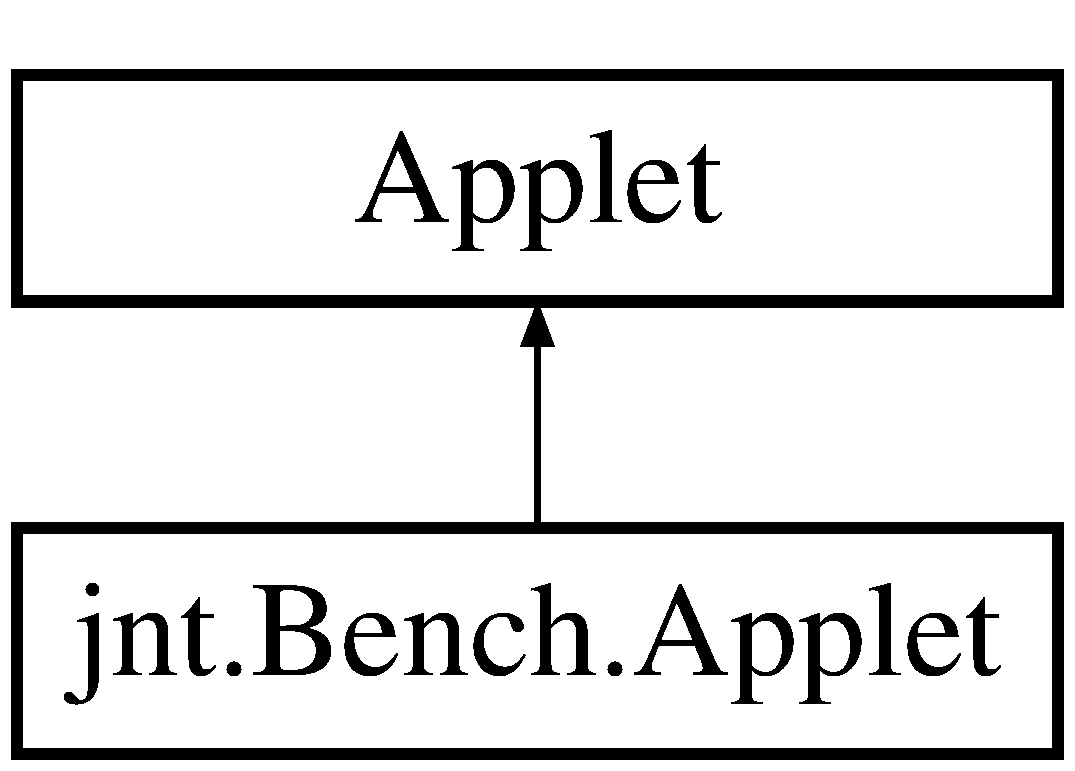
\includegraphics[height=2.000000cm]{d7/ddf/classjnt_1_1Bench_1_1Applet}
\end{center}
\end{figure}
\subsection*{Fonctions membres publiques}
\begin{DoxyCompactItemize}
\item 
void \hyperlink{classjnt_1_1Bench_1_1Applet_a54b7c975bcba940c87ccfa197c8a2b61}{init} ()
\item 
void \hyperlink{classjnt_1_1Bench_1_1Applet_a8c0a97f2e1d9b795203ca12e6c96fed8}{stop} ()
\item 
boolean \hyperlink{classjnt_1_1Bench_1_1Applet_a4b90b4d75bc1f2c082ff92826f599b36}{handle\-Event} (Event e)
\item 
void \hyperlink{classjnt_1_1Bench_1_1Applet_ab48d64c3129115fd26a2ffb2c5e971a8}{note\-Status} (String stat)
\end{DoxyCompactItemize}
\subsection*{Fonctions membres publiques statiques}
\begin{DoxyCompactItemize}
\item 
static void \hyperlink{classjnt_1_1Bench_1_1Applet_a51abb923fe907cb3156420f556c09b29}{main} (String args\mbox{[}$\,$\mbox{]})
\end{DoxyCompactItemize}


\subsection{Description détaillée}
\hyperlink{classjnt_1_1Bench_1_1Applet}{jnt.\-Bench.\-Applet} provides an \hyperlink{classjnt_1_1Bench_1_1Applet}{Applet} or Application with G\-U\-I to display and execute a benchmark implementing \hyperlink{interfacejnt_1_1Bench_1_1Target}{jnt.\-Bench.\-Target}.

\begin{DoxyAuthor}{Auteur}
Bruce R. Miller (\href{mailto:bruce.miller@nist.gov}{\tt bruce.\-miller@nist.\-gov}) 

Contribution of the National Institute of Standards and Technology, 

not subject to copyright. 
\end{DoxyAuthor}


\subsection{Documentation des fonctions membres}
\hypertarget{classjnt_1_1Bench_1_1Applet_a4b90b4d75bc1f2c082ff92826f599b36}{\index{jnt\-::\-Bench\-::\-Applet@{jnt\-::\-Bench\-::\-Applet}!handle\-Event@{handle\-Event}}
\index{handle\-Event@{handle\-Event}!jnt::Bench::Applet@{jnt\-::\-Bench\-::\-Applet}}
\subsubsection[{handle\-Event}]{\setlength{\rightskip}{0pt plus 5cm}boolean jnt.\-Bench.\-Applet.\-handle\-Event (
\begin{DoxyParamCaption}
\item[{Event}]{e}
\end{DoxyParamCaption}
)}}\label{classjnt_1_1Bench_1_1Applet_a4b90b4d75bc1f2c082ff92826f599b36}
Handling Events \hypertarget{classjnt_1_1Bench_1_1Applet_a54b7c975bcba940c87ccfa197c8a2b61}{\index{jnt\-::\-Bench\-::\-Applet@{jnt\-::\-Bench\-::\-Applet}!init@{init}}
\index{init@{init}!jnt::Bench::Applet@{jnt\-::\-Bench\-::\-Applet}}
\subsubsection[{init}]{\setlength{\rightskip}{0pt plus 5cm}void jnt.\-Bench.\-Applet.\-init (
\begin{DoxyParamCaption}
{}
\end{DoxyParamCaption}
)}}\label{classjnt_1_1Bench_1_1Applet_a54b7c975bcba940c87ccfa197c8a2b61}
\hypertarget{classjnt_1_1Bench_1_1Applet_a51abb923fe907cb3156420f556c09b29}{\index{jnt\-::\-Bench\-::\-Applet@{jnt\-::\-Bench\-::\-Applet}!main@{main}}
\index{main@{main}!jnt::Bench::Applet@{jnt\-::\-Bench\-::\-Applet}}
\subsubsection[{main}]{\setlength{\rightskip}{0pt plus 5cm}static void jnt.\-Bench.\-Applet.\-main (
\begin{DoxyParamCaption}
\item[{String}]{args\mbox{[}$\,$\mbox{]}}
\end{DoxyParamCaption}
)\hspace{0.3cm}{\ttfamily [static]}}}\label{classjnt_1_1Bench_1_1Applet_a51abb923fe907cb3156420f556c09b29}


 Running as application \hypertarget{classjnt_1_1Bench_1_1Applet_ab48d64c3129115fd26a2ffb2c5e971a8}{\index{jnt\-::\-Bench\-::\-Applet@{jnt\-::\-Bench\-::\-Applet}!note\-Status@{note\-Status}}
\index{note\-Status@{note\-Status}!jnt::Bench::Applet@{jnt\-::\-Bench\-::\-Applet}}
\subsubsection[{note\-Status}]{\setlength{\rightskip}{0pt plus 5cm}void jnt.\-Bench.\-Applet.\-note\-Status (
\begin{DoxyParamCaption}
\item[{String}]{stat}
\end{DoxyParamCaption}
)}}\label{classjnt_1_1Bench_1_1Applet_ab48d64c3129115fd26a2ffb2c5e971a8}
Callback to inform the applet of interesting status. \hypertarget{classjnt_1_1Bench_1_1Applet_a8c0a97f2e1d9b795203ca12e6c96fed8}{\index{jnt\-::\-Bench\-::\-Applet@{jnt\-::\-Bench\-::\-Applet}!stop@{stop}}
\index{stop@{stop}!jnt::Bench::Applet@{jnt\-::\-Bench\-::\-Applet}}
\subsubsection[{stop}]{\setlength{\rightskip}{0pt plus 5cm}void jnt.\-Bench.\-Applet.\-stop (
\begin{DoxyParamCaption}
{}
\end{DoxyParamCaption}
)}}\label{classjnt_1_1Bench_1_1Applet_a8c0a97f2e1d9b795203ca12e6c96fed8}


La documentation de cette classe a été générée à partir du fichier suivant \-:\begin{DoxyCompactItemize}
\item 
\hyperlink{Bench_2Applet_8java}{Bench/\-Applet.\-java}\end{DoxyCompactItemize}

\hypertarget{classjnt_1_1scimark2_1_1applet}{\section{Référence de la classe jnt.\-scimark2.\-applet}
\label{classjnt_1_1scimark2_1_1applet}\index{jnt.\-scimark2.\-applet@{jnt.\-scimark2.\-applet}}
}
Graphe d'héritage de jnt.\-scimark2.\-applet\-:\begin{figure}[H]
\begin{center}
\leavevmode
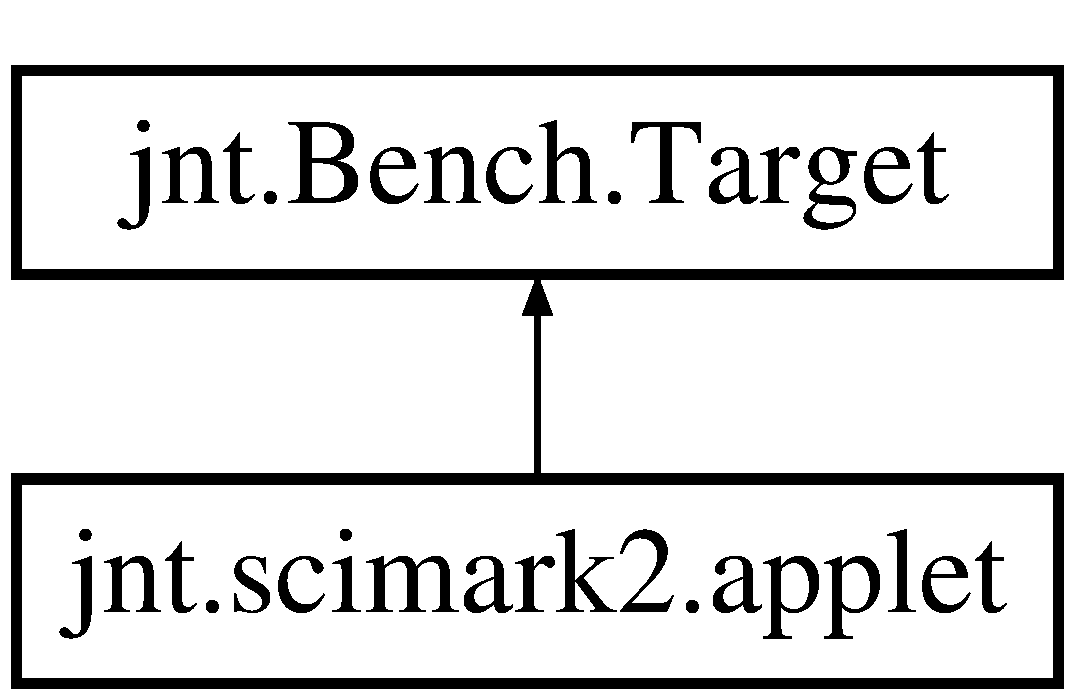
\includegraphics[height=2.000000cm]{dd/dfe/classjnt_1_1scimark2_1_1applet}
\end{center}
\end{figure}
\subsection*{Fonctions membres publiques}
\begin{DoxyCompactItemize}
\item 
double\mbox{[}$\,$\mbox{]} \hyperlink{classjnt_1_1scimark2_1_1applet_acc1746e5980a10c23f6f91d74f8b6136}{execute} (\hyperlink{classjnt_1_1Bench_1_1Bench}{jnt.\-Bench.\-Bench} b)
\end{DoxyCompactItemize}


\subsection{Documentation des fonctions membres}
\hypertarget{classjnt_1_1scimark2_1_1applet_acc1746e5980a10c23f6f91d74f8b6136}{\index{jnt\-::scimark2\-::applet@{jnt\-::scimark2\-::applet}!execute@{execute}}
\index{execute@{execute}!jnt::scimark2::applet@{jnt\-::scimark2\-::applet}}
\subsubsection[{execute}]{\setlength{\rightskip}{0pt plus 5cm}double \mbox{[}$\,$\mbox{]} jnt.\-scimark2.\-applet.\-execute (
\begin{DoxyParamCaption}
\item[{{\bf jnt.\-Bench.\-Bench}}]{bench}
\end{DoxyParamCaption}
)}}\label{classjnt_1_1scimark2_1_1applet_acc1746e5980a10c23f6f91d74f8b6136}
The code to be measured is placed in this method. \begin{DoxyReturn}{Renvoie}
null lets \hyperlink{classjnt_1_1Bench_1_1Bench}{jnt.\-Bench.\-Bench} handle the timings. Otherwise, return an array containing the one or more measured values. 
\end{DoxyReturn}
\begin{DoxySeeAlso}{Voir également}
\hyperlink{classjnt_1_1Bench_1_1Bench}{jnt.\-Bench.\-Bench} \mbox{[}start$\vert$stop$\vert$reset\mbox{]}Timer methods for measurement tools. 
\end{DoxySeeAlso}


Implémente \hyperlink{interfacejnt_1_1Bench_1_1Target_aa848f1ea6d28c6423b3b89d10482dabe}{jnt.\-Bench.\-Target}.



La documentation de cette classe a été générée à partir du fichier suivant \-:\begin{DoxyCompactItemize}
\item 
\hyperlink{scimark2_2Applet_8java}{scimark2/\-Applet.\-java}\end{DoxyCompactItemize}

\hypertarget{classjnt_1_1Bench_1_1Bench}{\section{Référence de la classe jnt.\-Bench.\-Bench}
\label{classjnt_1_1Bench_1_1Bench}\index{jnt.\-Bench.\-Bench@{jnt.\-Bench.\-Bench}}
}
Graphe d'héritage de jnt.\-Bench.\-Bench\-:\begin{figure}[H]
\begin{center}
\leavevmode
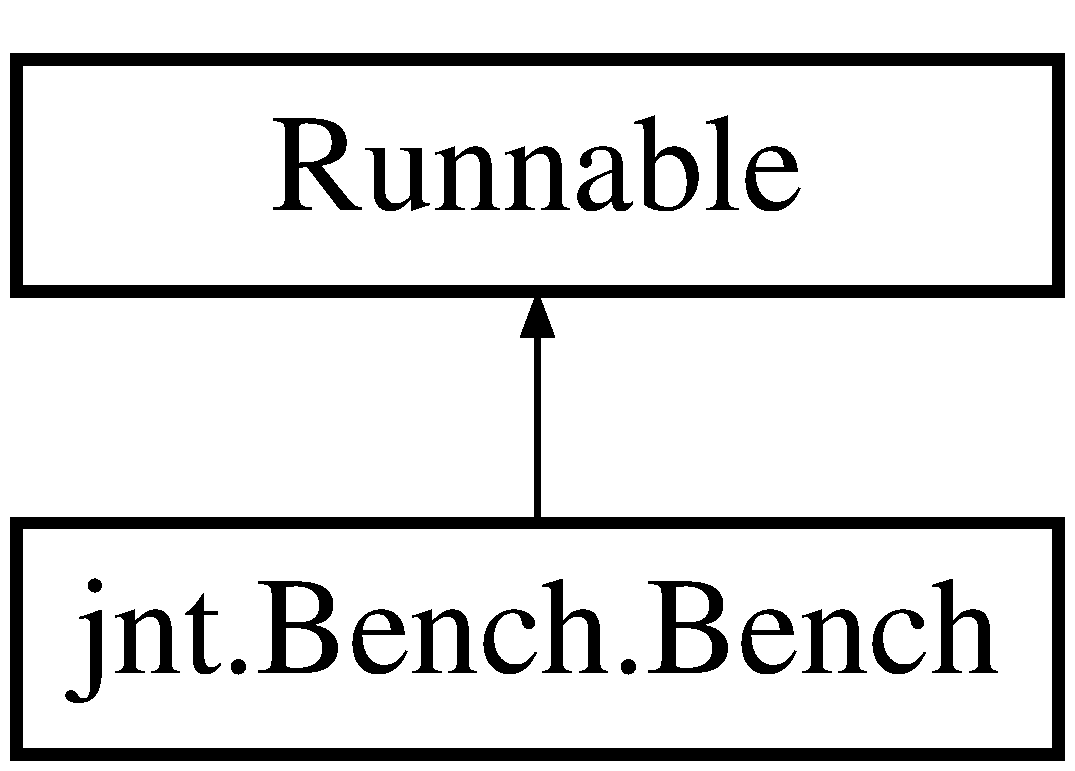
\includegraphics[height=2.000000cm]{d1/d59/classjnt_1_1Bench_1_1Bench}
\end{center}
\end{figure}
\subsection*{Fonctions membres publiques}
\begin{DoxyCompactItemize}
\item 
\hyperlink{classjnt_1_1Bench_1_1Bench_aff198cbca9a439e7a2da7a4cc59d0bd3}{Bench} (\hyperlink{classjnt_1_1Bench_1_1Applet}{Applet} applet, String filename)  throws I\-O\-Exception
\item 
\hyperlink{classjnt_1_1Bench_1_1Bench_a888aa428e2cc56203b892b90f2fd1cb3}{Bench} (\hyperlink{classjnt_1_1Bench_1_1Applet}{Applet} applet, U\-R\-L url)  throws I\-O\-Exception
\item 
\hyperlink{classjnt_1_1Bench_1_1Bench_a7945871dc162dd14c09c586ad6dd68ae}{Bench} (\hyperlink{classjnt_1_1Bench_1_1Applet}{Applet} applet, Input\-Stream stream)  throws I\-O\-Exception
\item 
String \hyperlink{classjnt_1_1Bench_1_1Bench_a042cccc7cb34a51489f02ea03380f11d}{get\-Name} ()
\item 
boolean \hyperlink{classjnt_1_1Bench_1_1Bench_a7f92ebd6cde5a2200f33918e572ad109}{is\-Runnable} ()
\item 
boolean \hyperlink{classjnt_1_1Bench_1_1Bench_ab93619fe34006f5b9711628bc9b7f553}{is\-Submittable} ()
\item 
String \hyperlink{classjnt_1_1Bench_1_1Bench_a6cfdde7ffbd8bc2b7d254df34d2010aa}{get\-Submissions\-Email} ()
\item 
String \hyperlink{classjnt_1_1Bench_1_1Bench_a338d608713cd03f88beaeac9175287fa}{get\-Submissions\-U\-R\-L} ()
\item 
int \hyperlink{classjnt_1_1Bench_1_1Bench_a1d7775686d5c5c3ec262935a40ac2d28}{get\-Special\-Pos} ()
\item 
int \hyperlink{classjnt_1_1Bench_1_1Bench_adb01f6f1c649cb97405b6e7293eb0af9}{get\-Num\-Segments} ()
\item 
String\mbox{[}$\,$\mbox{]} \hyperlink{classjnt_1_1Bench_1_1Bench_a99f0050c4666c8e0b184d26e32004a3e}{get\-Segment\-Names} ()
\item 
String \hyperlink{classjnt_1_1Bench_1_1Bench_ac2f2bd6fbe488bcc01e25c0605ebdfd8}{get\-Segment\-Units} (int seg)
\item 
String\mbox{[}$\,$\mbox{]} \hyperlink{classjnt_1_1Bench_1_1Bench_ae69d825062d634fd242e328fa938891c}{get\-Segment\-Units} ()
\item 
double\mbox{[}$\,$\mbox{]} \hyperlink{classjnt_1_1Bench_1_1Bench_a0cd263426221feadeb06a3261c512b7f}{get\-Segment\-Values} (int seg)
\item 
String\mbox{[}$\,$\mbox{]} \hyperlink{classjnt_1_1Bench_1_1Bench_a27eb6aee303297391d4db18e7292f393}{get\-Entries} ()
\item 
double\mbox{[}$\,$\mbox{]} \hyperlink{classjnt_1_1Bench_1_1Bench_af129c2c1c9f0fd0521c588fbe0858316}{get\-Current\-Values} ()
\item 
void \hyperlink{classjnt_1_1Bench_1_1Bench_adc4f56129d2d520fa053b6e897fae603}{start\-Timer} (int segment)
\item 
double \hyperlink{classjnt_1_1Bench_1_1Bench_ac2d936cd5bdbac44cbafd32b2d45bed5}{stop\-Timer} (int segment)
\item 
void \hyperlink{classjnt_1_1Bench_1_1Bench_a0c644e38e53da02d84e58de1699abdb0}{reset\-Timer} (int segment)
\item 
void \hyperlink{classjnt_1_1Bench_1_1Bench_ae16a57561b6556f5af23b8259a1eaad2}{resume\-Timer} (int segment)
\item 
void \hyperlink{classjnt_1_1Bench_1_1Bench_ac48b97a06575941423b1205eafee97b8}{note\-Status} (String stat)
\item 
void \hyperlink{classjnt_1_1Bench_1_1Bench_a9c4d4fd8e2c1683354606583b3cf34b2}{run} ()
\item 
void \hyperlink{classjnt_1_1Bench_1_1Bench_aaa30c2b9e9c2ceb32577f62797f25238}{print\-Measurements} (Print\-Stream out)
\item 
int \hyperlink{classjnt_1_1Bench_1_1Bench_a949dc538333236c1f4b56cf889b99e49}{get\-Special\-Rownum} ()
\item 
String\mbox{[}$\,$\mbox{]} \hyperlink{classjnt_1_1Bench_1_1Bench_a1e7862017e65305a9c156d7880b25448}{table\-Rows} ()
\end{DoxyCompactItemize}
\subsection*{Fonctions membres publiques statiques}
\begin{DoxyCompactItemize}
\item 
static void \hyperlink{classjnt_1_1Bench_1_1Bench_a95016eb20f5349e06fb6db2ccb78b2f9}{main} (String args\mbox{[}$\,$\mbox{]})  throws Exception 
\end{DoxyCompactItemize}


\subsection{Description détaillée}
A Description of a Benchmark.

Put description of Descriptor file here!!!

\begin{DoxyAuthor}{Auteur}
Bruce R. Miller (\href{mailto:bruce.miller@nist.gov}{\tt bruce.\-miller@nist.\-gov}) 

Contribution of the National Institute of Standards and Technology, 

not subject to copyright. 
\end{DoxyAuthor}


\subsection{Documentation des constructeurs et destructeur}
\hypertarget{classjnt_1_1Bench_1_1Bench_aff198cbca9a439e7a2da7a4cc59d0bd3}{\index{jnt\-::\-Bench\-::\-Bench@{jnt\-::\-Bench\-::\-Bench}!Bench@{Bench}}
\index{Bench@{Bench}!jnt::Bench::Bench@{jnt\-::\-Bench\-::\-Bench}}
\subsubsection[{Bench}]{\setlength{\rightskip}{0pt plus 5cm}jnt.\-Bench.\-Bench.\-Bench (
\begin{DoxyParamCaption}
\item[{{\bf Applet}}]{applet, }
\item[{String}]{filename}
\end{DoxyParamCaption}
) throws I\-O\-Exception}}\label{classjnt_1_1Bench_1_1Bench_aff198cbca9a439e7a2da7a4cc59d0bd3}
Create a Benchmark \hyperlink{classjnt_1_1Bench_1_1Bench}{Bench} based on the description in a file. \hypertarget{classjnt_1_1Bench_1_1Bench_a888aa428e2cc56203b892b90f2fd1cb3}{\index{jnt\-::\-Bench\-::\-Bench@{jnt\-::\-Bench\-::\-Bench}!Bench@{Bench}}
\index{Bench@{Bench}!jnt::Bench::Bench@{jnt\-::\-Bench\-::\-Bench}}
\subsubsection[{Bench}]{\setlength{\rightskip}{0pt plus 5cm}jnt.\-Bench.\-Bench.\-Bench (
\begin{DoxyParamCaption}
\item[{{\bf Applet}}]{applet, }
\item[{U\-R\-L}]{url}
\end{DoxyParamCaption}
) throws I\-O\-Exception}}\label{classjnt_1_1Bench_1_1Bench_a888aa428e2cc56203b892b90f2fd1cb3}
Create a Benchmark \hyperlink{classjnt_1_1Bench_1_1Bench}{Bench} based on the description in a U\-R\-L. \hypertarget{classjnt_1_1Bench_1_1Bench_a7945871dc162dd14c09c586ad6dd68ae}{\index{jnt\-::\-Bench\-::\-Bench@{jnt\-::\-Bench\-::\-Bench}!Bench@{Bench}}
\index{Bench@{Bench}!jnt::Bench::Bench@{jnt\-::\-Bench\-::\-Bench}}
\subsubsection[{Bench}]{\setlength{\rightskip}{0pt plus 5cm}jnt.\-Bench.\-Bench.\-Bench (
\begin{DoxyParamCaption}
\item[{{\bf Applet}}]{applet, }
\item[{Input\-Stream}]{stream}
\end{DoxyParamCaption}
) throws I\-O\-Exception}}\label{classjnt_1_1Bench_1_1Bench_a7945871dc162dd14c09c586ad6dd68ae}


\subsection{Documentation des fonctions membres}
\hypertarget{classjnt_1_1Bench_1_1Bench_af129c2c1c9f0fd0521c588fbe0858316}{\index{jnt\-::\-Bench\-::\-Bench@{jnt\-::\-Bench\-::\-Bench}!get\-Current\-Values@{get\-Current\-Values}}
\index{get\-Current\-Values@{get\-Current\-Values}!jnt::Bench::Bench@{jnt\-::\-Bench\-::\-Bench}}
\subsubsection[{get\-Current\-Values}]{\setlength{\rightskip}{0pt plus 5cm}double \mbox{[}$\,$\mbox{]} jnt.\-Bench.\-Bench.\-get\-Current\-Values (
\begin{DoxyParamCaption}
{}
\end{DoxyParamCaption}
)}}\label{classjnt_1_1Bench_1_1Bench_af129c2c1c9f0fd0521c588fbe0858316}
Return the measured values for the current measurement (if any) of this benchmark. \hypertarget{classjnt_1_1Bench_1_1Bench_a27eb6aee303297391d4db18e7292f393}{\index{jnt\-::\-Bench\-::\-Bench@{jnt\-::\-Bench\-::\-Bench}!get\-Entries@{get\-Entries}}
\index{get\-Entries@{get\-Entries}!jnt::Bench::Bench@{jnt\-::\-Bench\-::\-Bench}}
\subsubsection[{get\-Entries}]{\setlength{\rightskip}{0pt plus 5cm}String \mbox{[}$\,$\mbox{]} jnt.\-Bench.\-Bench.\-get\-Entries (
\begin{DoxyParamCaption}
{}
\end{DoxyParamCaption}
)}}\label{classjnt_1_1Bench_1_1Bench_a27eb6aee303297391d4db18e7292f393}
Return the platform names for all entries in this benchmark. \hypertarget{classjnt_1_1Bench_1_1Bench_a042cccc7cb34a51489f02ea03380f11d}{\index{jnt\-::\-Bench\-::\-Bench@{jnt\-::\-Bench\-::\-Bench}!get\-Name@{get\-Name}}
\index{get\-Name@{get\-Name}!jnt::Bench::Bench@{jnt\-::\-Bench\-::\-Bench}}
\subsubsection[{get\-Name}]{\setlength{\rightskip}{0pt plus 5cm}String jnt.\-Bench.\-Bench.\-get\-Name (
\begin{DoxyParamCaption}
{}
\end{DoxyParamCaption}
)}}\label{classjnt_1_1Bench_1_1Bench_a042cccc7cb34a51489f02ea03380f11d}


 Accessors for the Segment \& Entry information. Return the name of the benchmark target. \hypertarget{classjnt_1_1Bench_1_1Bench_adb01f6f1c649cb97405b6e7293eb0af9}{\index{jnt\-::\-Bench\-::\-Bench@{jnt\-::\-Bench\-::\-Bench}!get\-Num\-Segments@{get\-Num\-Segments}}
\index{get\-Num\-Segments@{get\-Num\-Segments}!jnt::Bench::Bench@{jnt\-::\-Bench\-::\-Bench}}
\subsubsection[{get\-Num\-Segments}]{\setlength{\rightskip}{0pt plus 5cm}int jnt.\-Bench.\-Bench.\-get\-Num\-Segments (
\begin{DoxyParamCaption}
{}
\end{DoxyParamCaption}
)}}\label{classjnt_1_1Bench_1_1Bench_adb01f6f1c649cb97405b6e7293eb0af9}
Return the number of segments in this benchmark. \hypertarget{classjnt_1_1Bench_1_1Bench_a99f0050c4666c8e0b184d26e32004a3e}{\index{jnt\-::\-Bench\-::\-Bench@{jnt\-::\-Bench\-::\-Bench}!get\-Segment\-Names@{get\-Segment\-Names}}
\index{get\-Segment\-Names@{get\-Segment\-Names}!jnt::Bench::Bench@{jnt\-::\-Bench\-::\-Bench}}
\subsubsection[{get\-Segment\-Names}]{\setlength{\rightskip}{0pt plus 5cm}String \mbox{[}$\,$\mbox{]} jnt.\-Bench.\-Bench.\-get\-Segment\-Names (
\begin{DoxyParamCaption}
{}
\end{DoxyParamCaption}
)}}\label{classjnt_1_1Bench_1_1Bench_a99f0050c4666c8e0b184d26e32004a3e}
Return the names of the segments in this benchmark. \hypertarget{classjnt_1_1Bench_1_1Bench_ac2f2bd6fbe488bcc01e25c0605ebdfd8}{\index{jnt\-::\-Bench\-::\-Bench@{jnt\-::\-Bench\-::\-Bench}!get\-Segment\-Units@{get\-Segment\-Units}}
\index{get\-Segment\-Units@{get\-Segment\-Units}!jnt::Bench::Bench@{jnt\-::\-Bench\-::\-Bench}}
\subsubsection[{get\-Segment\-Units}]{\setlength{\rightskip}{0pt plus 5cm}String jnt.\-Bench.\-Bench.\-get\-Segment\-Units (
\begin{DoxyParamCaption}
\item[{int}]{seg}
\end{DoxyParamCaption}
)}}\label{classjnt_1_1Bench_1_1Bench_ac2f2bd6fbe488bcc01e25c0605ebdfd8}
Return the units of segment seg in this benchmark. \hypertarget{classjnt_1_1Bench_1_1Bench_ae69d825062d634fd242e328fa938891c}{\index{jnt\-::\-Bench\-::\-Bench@{jnt\-::\-Bench\-::\-Bench}!get\-Segment\-Units@{get\-Segment\-Units}}
\index{get\-Segment\-Units@{get\-Segment\-Units}!jnt::Bench::Bench@{jnt\-::\-Bench\-::\-Bench}}
\subsubsection[{get\-Segment\-Units}]{\setlength{\rightskip}{0pt plus 5cm}String \mbox{[}$\,$\mbox{]} jnt.\-Bench.\-Bench.\-get\-Segment\-Units (
\begin{DoxyParamCaption}
{}
\end{DoxyParamCaption}
)}}\label{classjnt_1_1Bench_1_1Bench_ae69d825062d634fd242e328fa938891c}
Return the units of the segments in this benchmark. \hypertarget{classjnt_1_1Bench_1_1Bench_a0cd263426221feadeb06a3261c512b7f}{\index{jnt\-::\-Bench\-::\-Bench@{jnt\-::\-Bench\-::\-Bench}!get\-Segment\-Values@{get\-Segment\-Values}}
\index{get\-Segment\-Values@{get\-Segment\-Values}!jnt::Bench::Bench@{jnt\-::\-Bench\-::\-Bench}}
\subsubsection[{get\-Segment\-Values}]{\setlength{\rightskip}{0pt plus 5cm}double \mbox{[}$\,$\mbox{]} jnt.\-Bench.\-Bench.\-get\-Segment\-Values (
\begin{DoxyParamCaption}
\item[{int}]{seg}
\end{DoxyParamCaption}
)}}\label{classjnt_1_1Bench_1_1Bench_a0cd263426221feadeb06a3261c512b7f}
Return the measured values for all entries in segment seg in this benchmark. \hypertarget{classjnt_1_1Bench_1_1Bench_a1d7775686d5c5c3ec262935a40ac2d28}{\index{jnt\-::\-Bench\-::\-Bench@{jnt\-::\-Bench\-::\-Bench}!get\-Special\-Pos@{get\-Special\-Pos}}
\index{get\-Special\-Pos@{get\-Special\-Pos}!jnt::Bench::Bench@{jnt\-::\-Bench\-::\-Bench}}
\subsubsection[{get\-Special\-Pos}]{\setlength{\rightskip}{0pt plus 5cm}int jnt.\-Bench.\-Bench.\-get\-Special\-Pos (
\begin{DoxyParamCaption}
{}
\end{DoxyParamCaption}
)}}\label{classjnt_1_1Bench_1_1Bench_a1d7775686d5c5c3ec262935a40ac2d28}
Return the index of the Special Entry (the current system). \hypertarget{classjnt_1_1Bench_1_1Bench_a949dc538333236c1f4b56cf889b99e49}{\index{jnt\-::\-Bench\-::\-Bench@{jnt\-::\-Bench\-::\-Bench}!get\-Special\-Rownum@{get\-Special\-Rownum}}
\index{get\-Special\-Rownum@{get\-Special\-Rownum}!jnt::Bench::Bench@{jnt\-::\-Bench\-::\-Bench}}
\subsubsection[{get\-Special\-Rownum}]{\setlength{\rightskip}{0pt plus 5cm}int jnt.\-Bench.\-Bench.\-get\-Special\-Rownum (
\begin{DoxyParamCaption}
{}
\end{DoxyParamCaption}
)}}\label{classjnt_1_1Bench_1_1Bench_a949dc538333236c1f4b56cf889b99e49}
\hypertarget{classjnt_1_1Bench_1_1Bench_a6cfdde7ffbd8bc2b7d254df34d2010aa}{\index{jnt\-::\-Bench\-::\-Bench@{jnt\-::\-Bench\-::\-Bench}!get\-Submissions\-Email@{get\-Submissions\-Email}}
\index{get\-Submissions\-Email@{get\-Submissions\-Email}!jnt::Bench::Bench@{jnt\-::\-Bench\-::\-Bench}}
\subsubsection[{get\-Submissions\-Email}]{\setlength{\rightskip}{0pt plus 5cm}String jnt.\-Bench.\-Bench.\-get\-Submissions\-Email (
\begin{DoxyParamCaption}
{}
\end{DoxyParamCaption}
)}}\label{classjnt_1_1Bench_1_1Bench_a6cfdde7ffbd8bc2b7d254df34d2010aa}
Return the email address that submissions should be sent to. \hypertarget{classjnt_1_1Bench_1_1Bench_a338d608713cd03f88beaeac9175287fa}{\index{jnt\-::\-Bench\-::\-Bench@{jnt\-::\-Bench\-::\-Bench}!get\-Submissions\-U\-R\-L@{get\-Submissions\-U\-R\-L}}
\index{get\-Submissions\-U\-R\-L@{get\-Submissions\-U\-R\-L}!jnt::Bench::Bench@{jnt\-::\-Bench\-::\-Bench}}
\subsubsection[{get\-Submissions\-U\-R\-L}]{\setlength{\rightskip}{0pt plus 5cm}String jnt.\-Bench.\-Bench.\-get\-Submissions\-U\-R\-L (
\begin{DoxyParamCaption}
{}
\end{DoxyParamCaption}
)}}\label{classjnt_1_1Bench_1_1Bench_a338d608713cd03f88beaeac9175287fa}
Return the url that submissions should be posted to. \hypertarget{classjnt_1_1Bench_1_1Bench_a7f92ebd6cde5a2200f33918e572ad109}{\index{jnt\-::\-Bench\-::\-Bench@{jnt\-::\-Bench\-::\-Bench}!is\-Runnable@{is\-Runnable}}
\index{is\-Runnable@{is\-Runnable}!jnt::Bench::Bench@{jnt\-::\-Bench\-::\-Bench}}
\subsubsection[{is\-Runnable}]{\setlength{\rightskip}{0pt plus 5cm}boolean jnt.\-Bench.\-Bench.\-is\-Runnable (
\begin{DoxyParamCaption}
{}
\end{DoxyParamCaption}
)}}\label{classjnt_1_1Bench_1_1Bench_a7f92ebd6cde5a2200f33918e572ad109}
Return whether the benchmark \hyperlink{interfacejnt_1_1Bench_1_1Target}{Target} is (likely) runnable. \hypertarget{classjnt_1_1Bench_1_1Bench_ab93619fe34006f5b9711628bc9b7f553}{\index{jnt\-::\-Bench\-::\-Bench@{jnt\-::\-Bench\-::\-Bench}!is\-Submittable@{is\-Submittable}}
\index{is\-Submittable@{is\-Submittable}!jnt::Bench::Bench@{jnt\-::\-Bench\-::\-Bench}}
\subsubsection[{is\-Submittable}]{\setlength{\rightskip}{0pt plus 5cm}boolean jnt.\-Bench.\-Bench.\-is\-Submittable (
\begin{DoxyParamCaption}
{}
\end{DoxyParamCaption}
)}}\label{classjnt_1_1Bench_1_1Bench_ab93619fe34006f5b9711628bc9b7f553}
Return whether the benchmark results are submittable. \hypertarget{classjnt_1_1Bench_1_1Bench_a95016eb20f5349e06fb6db2ccb78b2f9}{\index{jnt\-::\-Bench\-::\-Bench@{jnt\-::\-Bench\-::\-Bench}!main@{main}}
\index{main@{main}!jnt::Bench::Bench@{jnt\-::\-Bench\-::\-Bench}}
\subsubsection[{main}]{\setlength{\rightskip}{0pt plus 5cm}static void jnt.\-Bench.\-Bench.\-main (
\begin{DoxyParamCaption}
\item[{String}]{args\mbox{[}$\,$\mbox{]}}
\end{DoxyParamCaption}
) throws Exception\hspace{0.3cm}{\ttfamily [static]}}}\label{classjnt_1_1Bench_1_1Bench_a95016eb20f5349e06fb6db2ccb78b2f9}
Run a Benchmark as a command-\/line application (without a G\-U\-I) \hypertarget{classjnt_1_1Bench_1_1Bench_ac48b97a06575941423b1205eafee97b8}{\index{jnt\-::\-Bench\-::\-Bench@{jnt\-::\-Bench\-::\-Bench}!note\-Status@{note\-Status}}
\index{note\-Status@{note\-Status}!jnt::Bench::Bench@{jnt\-::\-Bench\-::\-Bench}}
\subsubsection[{note\-Status}]{\setlength{\rightskip}{0pt plus 5cm}void jnt.\-Bench.\-Bench.\-note\-Status (
\begin{DoxyParamCaption}
\item[{String}]{stat}
\end{DoxyParamCaption}
)}}\label{classjnt_1_1Bench_1_1Bench_ac48b97a06575941423b1205eafee97b8}
Callback to inform us of interesting status. \hypertarget{classjnt_1_1Bench_1_1Bench_aaa30c2b9e9c2ceb32577f62797f25238}{\index{jnt\-::\-Bench\-::\-Bench@{jnt\-::\-Bench\-::\-Bench}!print\-Measurements@{print\-Measurements}}
\index{print\-Measurements@{print\-Measurements}!jnt::Bench::Bench@{jnt\-::\-Bench\-::\-Bench}}
\subsubsection[{print\-Measurements}]{\setlength{\rightskip}{0pt plus 5cm}void jnt.\-Bench.\-Bench.\-print\-Measurements (
\begin{DoxyParamCaption}
\item[{Print\-Stream}]{out}
\end{DoxyParamCaption}
)}}\label{classjnt_1_1Bench_1_1Bench_aaa30c2b9e9c2ceb32577f62797f25238}
\hypertarget{classjnt_1_1Bench_1_1Bench_a0c644e38e53da02d84e58de1699abdb0}{\index{jnt\-::\-Bench\-::\-Bench@{jnt\-::\-Bench\-::\-Bench}!reset\-Timer@{reset\-Timer}}
\index{reset\-Timer@{reset\-Timer}!jnt::Bench::Bench@{jnt\-::\-Bench\-::\-Bench}}
\subsubsection[{reset\-Timer}]{\setlength{\rightskip}{0pt plus 5cm}void jnt.\-Bench.\-Bench.\-reset\-Timer (
\begin{DoxyParamCaption}
\item[{int}]{segment}
\end{DoxyParamCaption}
)}}\label{classjnt_1_1Bench_1_1Bench_a0c644e38e53da02d84e58de1699abdb0}
Reset the timer for this segment. This is intended to be used as a callback from \hyperlink{interfacejnt_1_1Bench_1_1Target}{Target}. \hypertarget{classjnt_1_1Bench_1_1Bench_ae16a57561b6556f5af23b8259a1eaad2}{\index{jnt\-::\-Bench\-::\-Bench@{jnt\-::\-Bench\-::\-Bench}!resume\-Timer@{resume\-Timer}}
\index{resume\-Timer@{resume\-Timer}!jnt::Bench::Bench@{jnt\-::\-Bench\-::\-Bench}}
\subsubsection[{resume\-Timer}]{\setlength{\rightskip}{0pt plus 5cm}void jnt.\-Bench.\-Bench.\-resume\-Timer (
\begin{DoxyParamCaption}
\item[{int}]{segment}
\end{DoxyParamCaption}
)}}\label{classjnt_1_1Bench_1_1Bench_ae16a57561b6556f5af23b8259a1eaad2}
Resume the timer for segment. This is like starting the timer without resetting it first. This is intended to be used as a callback from \hyperlink{interfacejnt_1_1Bench_1_1Target}{Target}. \hypertarget{classjnt_1_1Bench_1_1Bench_a9c4d4fd8e2c1683354606583b3cf34b2}{\index{jnt\-::\-Bench\-::\-Bench@{jnt\-::\-Bench\-::\-Bench}!run@{run}}
\index{run@{run}!jnt::Bench::Bench@{jnt\-::\-Bench\-::\-Bench}}
\subsubsection[{run}]{\setlength{\rightskip}{0pt plus 5cm}void jnt.\-Bench.\-Bench.\-run (
\begin{DoxyParamCaption}
{}
\end{DoxyParamCaption}
)}}\label{classjnt_1_1Bench_1_1Bench_a9c4d4fd8e2c1683354606583b3cf34b2}
\hypertarget{classjnt_1_1Bench_1_1Bench_adc4f56129d2d520fa053b6e897fae603}{\index{jnt\-::\-Bench\-::\-Bench@{jnt\-::\-Bench\-::\-Bench}!start\-Timer@{start\-Timer}}
\index{start\-Timer@{start\-Timer}!jnt::Bench::Bench@{jnt\-::\-Bench\-::\-Bench}}
\subsubsection[{start\-Timer}]{\setlength{\rightskip}{0pt plus 5cm}void jnt.\-Bench.\-Bench.\-start\-Timer (
\begin{DoxyParamCaption}
\item[{int}]{segment}
\end{DoxyParamCaption}
)}}\label{classjnt_1_1Bench_1_1Bench_adc4f56129d2d520fa053b6e897fae603}
Start the timer for segment. It resets the timer for this segment if any previous measurement had been made. This is intended to be used as a callback from \hyperlink{interfacejnt_1_1Bench_1_1Target}{Target}. \hypertarget{classjnt_1_1Bench_1_1Bench_ac2d936cd5bdbac44cbafd32b2d45bed5}{\index{jnt\-::\-Bench\-::\-Bench@{jnt\-::\-Bench\-::\-Bench}!stop\-Timer@{stop\-Timer}}
\index{stop\-Timer@{stop\-Timer}!jnt::Bench::Bench@{jnt\-::\-Bench\-::\-Bench}}
\subsubsection[{stop\-Timer}]{\setlength{\rightskip}{0pt plus 5cm}double jnt.\-Bench.\-Bench.\-stop\-Timer (
\begin{DoxyParamCaption}
\item[{int}]{segment}
\end{DoxyParamCaption}
)}}\label{classjnt_1_1Bench_1_1Bench_ac2d936cd5bdbac44cbafd32b2d45bed5}
Stop the timer for this segment. It returns the timing, up to this point. This is intended to be used as a callback from \hyperlink{interfacejnt_1_1Bench_1_1Target}{Target}. \hypertarget{classjnt_1_1Bench_1_1Bench_a1e7862017e65305a9c156d7880b25448}{\index{jnt\-::\-Bench\-::\-Bench@{jnt\-::\-Bench\-::\-Bench}!table\-Rows@{table\-Rows}}
\index{table\-Rows@{table\-Rows}!jnt::Bench::Bench@{jnt\-::\-Bench\-::\-Bench}}
\subsubsection[{table\-Rows}]{\setlength{\rightskip}{0pt plus 5cm}String \mbox{[}$\,$\mbox{]} jnt.\-Bench.\-Bench.\-table\-Rows (
\begin{DoxyParamCaption}
{}
\end{DoxyParamCaption}
)}}\label{classjnt_1_1Bench_1_1Bench_a1e7862017e65305a9c156d7880b25448}
Return an array of strings representing the rows of a table tabulating the values in the benchmark. 

La documentation de cette classe a été générée à partir du fichier suivant \-:\begin{DoxyCompactItemize}
\item 
\hyperlink{Bench_8java}{Bench.\-java}\end{DoxyCompactItemize}

\hypertarget{classjnt_1_1BenchMark}{\section{Référence de la classe jnt.\-Bench\-Mark}
\label{classjnt_1_1BenchMark}\index{jnt.\-Bench\-Mark@{jnt.\-Bench\-Mark}}
}
\subsection*{Fonctions membres publiques}
\begin{DoxyCompactItemize}
\item 
\hyperlink{classjnt_1_1BenchMark_a675ba55b21fb6d0a3a169d769df11a23}{Bench\-Mark} (\hyperlink{interfacejnt_1_1BenchMarkResultEvent}{Bench\-Mark\-Result\-Event} \hyperlink{classjnt_1_1BenchMark_abcb332d393fba2c18c7cb700bd651366}{event})
\item 
void \hyperlink{classjnt_1_1BenchMark_a3f04e42ad806345973e12d04b4601315}{launch} ()
\end{DoxyCompactItemize}
\subsection*{Attributs privés}
\begin{DoxyCompactItemize}
\item 
\hyperlink{interfacejnt_1_1BenchMarkResultEvent}{Bench\-Mark\-Result\-Event} \hyperlink{classjnt_1_1BenchMark_abcb332d393fba2c18c7cb700bd651366}{event}
\end{DoxyCompactItemize}


\subsection{Description détaillée}
Sci\-Mark2\-: A Java numerical benchmark measuring performance of computational kernels for F\-F\-Ts, Monte Carlo simulation, sparse matrix computations, Jacobi S\-O\-R, and dense L\-U matrix factorizations.

\href{http://math.nist.gov/scimark2/index.html}{\tt http\-://math.\-nist.\-gov/scimark2/index.\-html} Ce module de \hyperlink{classjnt_1_1BenchMark}{Bench\-Mark} est une reprise de celui créée par Roldan Pozo et Bruce Miller \begin{DoxySeeAlso}{Voir également}
\href{http://math.nist.gov/scimark2/}{\tt Site web} \par
 Classe qui va permettre de gérer le module de Bench\-Marking 
\end{DoxySeeAlso}
\begin{DoxyAuthor}{Auteur}

\begin{DoxyItemize}
\item Morgane Badré 
\item Vincent Wilmet 
\end{DoxyItemize}
\end{DoxyAuthor}
\begin{DoxyVersion}{Version}
1.\-0 
\end{DoxyVersion}


\subsection{Documentation des constructeurs et destructeur}
\hypertarget{classjnt_1_1BenchMark_a675ba55b21fb6d0a3a169d769df11a23}{\index{jnt\-::\-Bench\-Mark@{jnt\-::\-Bench\-Mark}!Bench\-Mark@{Bench\-Mark}}
\index{Bench\-Mark@{Bench\-Mark}!jnt::BenchMark@{jnt\-::\-Bench\-Mark}}
\subsubsection[{Bench\-Mark}]{\setlength{\rightskip}{0pt plus 5cm}jnt.\-Bench\-Mark.\-Bench\-Mark (
\begin{DoxyParamCaption}
\item[{{\bf Bench\-Mark\-Result\-Event}}]{event}
\end{DoxyParamCaption}
)}}\label{classjnt_1_1BenchMark_a675ba55b21fb6d0a3a169d769df11a23}
Constructeur qui neccessite l'utilisation de l'interface afin de communiqué les résultats du calcul {\bfseries Attention \-: }Vous devez fournir une référence valide pour l'objet en paramètre sinon il seras impossible de connaitre l'avancement du calcul général et de récupèrer les valeurs finales 
\begin{DoxyParams}{Paramètres}
{\em event} & L'interface de communication avec le \hyperlink{classjnt_1_1BenchMark}{Bench\-Mark} \\
\hline
\end{DoxyParams}


\subsection{Documentation des fonctions membres}
\hypertarget{classjnt_1_1BenchMark_a3f04e42ad806345973e12d04b4601315}{\index{jnt\-::\-Bench\-Mark@{jnt\-::\-Bench\-Mark}!launch@{launch}}
\index{launch@{launch}!jnt::BenchMark@{jnt\-::\-Bench\-Mark}}
\subsubsection[{launch}]{\setlength{\rightskip}{0pt plus 5cm}void jnt.\-Bench\-Mark.\-launch (
\begin{DoxyParamCaption}
{}
\end{DoxyParamCaption}
)}}\label{classjnt_1_1BenchMark_a3f04e42ad806345973e12d04b4601315}
Méthode à appeler afin de lancer le Bench\-Marking \par
 Cette méthode renvoie à travers l'objet passé en paramètre du constructeur de l'interface \hyperlink{interfacejnt_1_1BenchMarkResultEvent}{jnt.\-Bench\-Mark\-Result\-Event} \par
 Si l'interface de communication n'est pas valide alors le Bench\-Marking ne se lance pas et s'arrète immédiatement 

\subsection{Documentation des données membres}
\hypertarget{classjnt_1_1BenchMark_abcb332d393fba2c18c7cb700bd651366}{\index{jnt\-::\-Bench\-Mark@{jnt\-::\-Bench\-Mark}!event@{event}}
\index{event@{event}!jnt::BenchMark@{jnt\-::\-Bench\-Mark}}
\subsubsection[{event}]{\setlength{\rightskip}{0pt plus 5cm}{\bf Bench\-Mark\-Result\-Event} jnt.\-Bench\-Mark.\-event\hspace{0.3cm}{\ttfamily [private]}}}\label{classjnt_1_1BenchMark_abcb332d393fba2c18c7cb700bd651366}
Interface qui permet la comuniquation ainsi que de d'informer de l'avancement des calculs du Bench\-Marking 

La documentation de cette classe a été générée à partir du fichier suivant \-:\begin{DoxyCompactItemize}
\item 
\hyperlink{BenchMark_8java}{Bench\-Mark.\-java}\end{DoxyCompactItemize}

\hypertarget{classjnt_1_1BenchMarkResult}{\section{Référence de la classe jnt.\-Bench\-Mark\-Result}
\label{classjnt_1_1BenchMarkResult}\index{jnt.\-Bench\-Mark\-Result@{jnt.\-Bench\-Mark\-Result}}
}
\subsection*{Classes}
\begin{DoxyCompactItemize}
\item 
class \hyperlink{classjnt_1_1BenchMarkResult_1_1FFT}{F\-F\-T}
\item 
class \hyperlink{classjnt_1_1BenchMarkResult_1_1LU}{L\-U}
\item 
class \hyperlink{classjnt_1_1BenchMarkResult_1_1MonteCarlo}{Monte\-Carlo}
\item 
class \hyperlink{classjnt_1_1BenchMarkResult_1_1SOR}{S\-O\-R}
\item 
class \hyperlink{classjnt_1_1BenchMarkResult_1_1SparseMatmult}{Sparse\-Matmult}
\end{DoxyCompactItemize}
\subsection*{Fonctions membres publiques}
\begin{DoxyCompactItemize}
\item 
void \hyperlink{classjnt_1_1BenchMarkResult_a0045bf62b5b5d7a0814779b6ad798800}{set\-F\-F\-T} (\hyperlink{classjnt_1_1BenchMarkResult_1_1FFT}{F\-F\-T} \hyperlink{classjnt_1_1BenchMarkResult_a4ccbb09fa780dd422598546e86c845d7}{fft})
\item 
void \hyperlink{classjnt_1_1BenchMarkResult_af84c3e1f64ba2cef7fbe5756cce7454d}{set\-S\-O\-R} (\hyperlink{classjnt_1_1BenchMarkResult_1_1SOR}{S\-O\-R} \hyperlink{classjnt_1_1BenchMarkResult_a159025733607bd514927639795a47971}{sor})
\item 
void \hyperlink{classjnt_1_1BenchMarkResult_a15deedb34ecfdfb1bd5ee588c9a5c612}{set\-Monte\-Carlo} (\hyperlink{classjnt_1_1BenchMarkResult_1_1MonteCarlo}{Monte\-Carlo} \hyperlink{classjnt_1_1BenchMarkResult_a9f32de31bdbd4ecdf9ea3832825e0ba8}{monte\-Carlo})
\item 
void \hyperlink{classjnt_1_1BenchMarkResult_a9dc60916021b2fa2a0c14df14f679358}{set\-Sparse\-Matmult} (\hyperlink{classjnt_1_1BenchMarkResult_1_1SparseMatmult}{Sparse\-Matmult} \hyperlink{classjnt_1_1BenchMarkResult_abd6ec31f144598923f60d2cc0040df95}{sparse\-Matmult})
\item 
void \hyperlink{classjnt_1_1BenchMarkResult_a8345a1091a25eb9ef91eca88ddd7bce7}{set\-L\-U} (\hyperlink{classjnt_1_1BenchMarkResult_1_1LU}{L\-U} \hyperlink{classjnt_1_1BenchMarkResult_a615ece215df7fa40fa3de24fb62a8d7c}{lu})
\item 
void \hyperlink{classjnt_1_1BenchMarkResult_a7fafc6b9c2bd5b2e6777e4fe2013b539}{set\-Scrore} (double score)
\item 
String \hyperlink{classjnt_1_1BenchMarkResult_a29d58433604078d4c1f205f9dac46930}{to\-String} ()
\end{DoxyCompactItemize}
\subsection*{Attributs publics}
\begin{DoxyCompactItemize}
\item 
\hyperlink{classjnt_1_1BenchMarkResult_1_1FFT}{F\-F\-T} \hyperlink{classjnt_1_1BenchMarkResult_a4ccbb09fa780dd422598546e86c845d7}{fft}
\item 
\hyperlink{classjnt_1_1BenchMarkResult_1_1SOR}{S\-O\-R} \hyperlink{classjnt_1_1BenchMarkResult_a159025733607bd514927639795a47971}{sor}
\item 
\hyperlink{classjnt_1_1BenchMarkResult_1_1MonteCarlo}{Monte\-Carlo} \hyperlink{classjnt_1_1BenchMarkResult_a9f32de31bdbd4ecdf9ea3832825e0ba8}{monte\-Carlo}
\item 
\hyperlink{classjnt_1_1BenchMarkResult_1_1SparseMatmult}{Sparse\-Matmult} \hyperlink{classjnt_1_1BenchMarkResult_abd6ec31f144598923f60d2cc0040df95}{sparse\-Matmult}
\item 
\hyperlink{classjnt_1_1BenchMarkResult_1_1LU}{L\-U} \hyperlink{classjnt_1_1BenchMarkResult_a615ece215df7fa40fa3de24fb62a8d7c}{lu}
\item 
double \hyperlink{classjnt_1_1BenchMarkResult_aaea8ab4bb0f7f2fa52f719b0846c3a84}{global\-Score}
\end{DoxyCompactItemize}


\subsection{Description détaillée}
Classe qui va contenir les résultats du Bench\-Marking \begin{DoxyAuthor}{Auteur}

\begin{DoxyItemize}
\item Morgane Badré 
\item Vincent Wilmet 
\end{DoxyItemize}
\end{DoxyAuthor}
\begin{DoxyVersion}{Version}
1.\-0 
\end{DoxyVersion}


\subsection{Documentation des fonctions membres}
\hypertarget{classjnt_1_1BenchMarkResult_a0045bf62b5b5d7a0814779b6ad798800}{\index{jnt\-::\-Bench\-Mark\-Result@{jnt\-::\-Bench\-Mark\-Result}!set\-F\-F\-T@{set\-F\-F\-T}}
\index{set\-F\-F\-T@{set\-F\-F\-T}!jnt::BenchMarkResult@{jnt\-::\-Bench\-Mark\-Result}}
\subsubsection[{set\-F\-F\-T}]{\setlength{\rightskip}{0pt plus 5cm}void jnt.\-Bench\-Mark\-Result.\-set\-F\-F\-T (
\begin{DoxyParamCaption}
\item[{{\bf F\-F\-T}}]{fft}
\end{DoxyParamCaption}
)}}\label{classjnt_1_1BenchMarkResult_a0045bf62b5b5d7a0814779b6ad798800}
Setter 
\begin{DoxyParams}{Paramètres}
{\em fft} & \\
\hline
\end{DoxyParams}
\hypertarget{classjnt_1_1BenchMarkResult_a8345a1091a25eb9ef91eca88ddd7bce7}{\index{jnt\-::\-Bench\-Mark\-Result@{jnt\-::\-Bench\-Mark\-Result}!set\-L\-U@{set\-L\-U}}
\index{set\-L\-U@{set\-L\-U}!jnt::BenchMarkResult@{jnt\-::\-Bench\-Mark\-Result}}
\subsubsection[{set\-L\-U}]{\setlength{\rightskip}{0pt plus 5cm}void jnt.\-Bench\-Mark\-Result.\-set\-L\-U (
\begin{DoxyParamCaption}
\item[{{\bf L\-U}}]{lu}
\end{DoxyParamCaption}
)}}\label{classjnt_1_1BenchMarkResult_a8345a1091a25eb9ef91eca88ddd7bce7}
Setter 
\begin{DoxyParams}{Paramètres}
{\em lu} & \\
\hline
\end{DoxyParams}
\hypertarget{classjnt_1_1BenchMarkResult_a15deedb34ecfdfb1bd5ee588c9a5c612}{\index{jnt\-::\-Bench\-Mark\-Result@{jnt\-::\-Bench\-Mark\-Result}!set\-Monte\-Carlo@{set\-Monte\-Carlo}}
\index{set\-Monte\-Carlo@{set\-Monte\-Carlo}!jnt::BenchMarkResult@{jnt\-::\-Bench\-Mark\-Result}}
\subsubsection[{set\-Monte\-Carlo}]{\setlength{\rightskip}{0pt plus 5cm}void jnt.\-Bench\-Mark\-Result.\-set\-Monte\-Carlo (
\begin{DoxyParamCaption}
\item[{{\bf Monte\-Carlo}}]{monte\-Carlo}
\end{DoxyParamCaption}
)}}\label{classjnt_1_1BenchMarkResult_a15deedb34ecfdfb1bd5ee588c9a5c612}
Setter 
\begin{DoxyParams}{Paramètres}
{\em monte\-Carlo} & \\
\hline
\end{DoxyParams}
\hypertarget{classjnt_1_1BenchMarkResult_a7fafc6b9c2bd5b2e6777e4fe2013b539}{\index{jnt\-::\-Bench\-Mark\-Result@{jnt\-::\-Bench\-Mark\-Result}!set\-Scrore@{set\-Scrore}}
\index{set\-Scrore@{set\-Scrore}!jnt::BenchMarkResult@{jnt\-::\-Bench\-Mark\-Result}}
\subsubsection[{set\-Scrore}]{\setlength{\rightskip}{0pt plus 5cm}void jnt.\-Bench\-Mark\-Result.\-set\-Scrore (
\begin{DoxyParamCaption}
\item[{double}]{score}
\end{DoxyParamCaption}
)}}\label{classjnt_1_1BenchMarkResult_a7fafc6b9c2bd5b2e6777e4fe2013b539}
Setter du score maximale 
\begin{DoxyParams}{Paramètres}
{\em score} & Le score global final \\
\hline
\end{DoxyParams}
\hypertarget{classjnt_1_1BenchMarkResult_af84c3e1f64ba2cef7fbe5756cce7454d}{\index{jnt\-::\-Bench\-Mark\-Result@{jnt\-::\-Bench\-Mark\-Result}!set\-S\-O\-R@{set\-S\-O\-R}}
\index{set\-S\-O\-R@{set\-S\-O\-R}!jnt::BenchMarkResult@{jnt\-::\-Bench\-Mark\-Result}}
\subsubsection[{set\-S\-O\-R}]{\setlength{\rightskip}{0pt plus 5cm}void jnt.\-Bench\-Mark\-Result.\-set\-S\-O\-R (
\begin{DoxyParamCaption}
\item[{{\bf S\-O\-R}}]{sor}
\end{DoxyParamCaption}
)}}\label{classjnt_1_1BenchMarkResult_af84c3e1f64ba2cef7fbe5756cce7454d}
Setter 
\begin{DoxyParams}{Paramètres}
{\em sor} & \\
\hline
\end{DoxyParams}
\hypertarget{classjnt_1_1BenchMarkResult_a9dc60916021b2fa2a0c14df14f679358}{\index{jnt\-::\-Bench\-Mark\-Result@{jnt\-::\-Bench\-Mark\-Result}!set\-Sparse\-Matmult@{set\-Sparse\-Matmult}}
\index{set\-Sparse\-Matmult@{set\-Sparse\-Matmult}!jnt::BenchMarkResult@{jnt\-::\-Bench\-Mark\-Result}}
\subsubsection[{set\-Sparse\-Matmult}]{\setlength{\rightskip}{0pt plus 5cm}void jnt.\-Bench\-Mark\-Result.\-set\-Sparse\-Matmult (
\begin{DoxyParamCaption}
\item[{{\bf Sparse\-Matmult}}]{sparse\-Matmult}
\end{DoxyParamCaption}
)}}\label{classjnt_1_1BenchMarkResult_a9dc60916021b2fa2a0c14df14f679358}
Setter 
\begin{DoxyParams}{Paramètres}
{\em sparse\-Matmult} & \\
\hline
\end{DoxyParams}
\hypertarget{classjnt_1_1BenchMarkResult_a29d58433604078d4c1f205f9dac46930}{\index{jnt\-::\-Bench\-Mark\-Result@{jnt\-::\-Bench\-Mark\-Result}!to\-String@{to\-String}}
\index{to\-String@{to\-String}!jnt::BenchMarkResult@{jnt\-::\-Bench\-Mark\-Result}}
\subsubsection[{to\-String}]{\setlength{\rightskip}{0pt plus 5cm}String jnt.\-Bench\-Mark\-Result.\-to\-String (
\begin{DoxyParamCaption}
{}
\end{DoxyParamCaption}
)}}\label{classjnt_1_1BenchMarkResult_a29d58433604078d4c1f205f9dac46930}
Méthode pour retourner en chaîne de caractères les résultats de chaques calculs 

\subsection{Documentation des données membres}
\hypertarget{classjnt_1_1BenchMarkResult_a4ccbb09fa780dd422598546e86c845d7}{\index{jnt\-::\-Bench\-Mark\-Result@{jnt\-::\-Bench\-Mark\-Result}!fft@{fft}}
\index{fft@{fft}!jnt::BenchMarkResult@{jnt\-::\-Bench\-Mark\-Result}}
\subsubsection[{fft}]{\setlength{\rightskip}{0pt plus 5cm}{\bf F\-F\-T} jnt.\-Bench\-Mark\-Result.\-fft}}\label{classjnt_1_1BenchMarkResult_a4ccbb09fa780dd422598546e86c845d7}
Objet de la classe \-: \hyperlink{classjnt_1_1BenchMarkResult_1_1FFT}{jnt.\-Bench\-Mark\-Result.\-F\-F\-T} \hypertarget{classjnt_1_1BenchMarkResult_aaea8ab4bb0f7f2fa52f719b0846c3a84}{\index{jnt\-::\-Bench\-Mark\-Result@{jnt\-::\-Bench\-Mark\-Result}!global\-Score@{global\-Score}}
\index{global\-Score@{global\-Score}!jnt::BenchMarkResult@{jnt\-::\-Bench\-Mark\-Result}}
\subsubsection[{global\-Score}]{\setlength{\rightskip}{0pt plus 5cm}double jnt.\-Bench\-Mark\-Result.\-global\-Score}}\label{classjnt_1_1BenchMarkResult_aaea8ab4bb0f7f2fa52f719b0846c3a84}
Réel qui va contenir le résultat finale. Celui ci est calculée en faiant la moyenne de tous les autres résultats \hypertarget{classjnt_1_1BenchMarkResult_a615ece215df7fa40fa3de24fb62a8d7c}{\index{jnt\-::\-Bench\-Mark\-Result@{jnt\-::\-Bench\-Mark\-Result}!lu@{lu}}
\index{lu@{lu}!jnt::BenchMarkResult@{jnt\-::\-Bench\-Mark\-Result}}
\subsubsection[{lu}]{\setlength{\rightskip}{0pt plus 5cm}{\bf L\-U} jnt.\-Bench\-Mark\-Result.\-lu}}\label{classjnt_1_1BenchMarkResult_a615ece215df7fa40fa3de24fb62a8d7c}
Objet de la classe \-: \hyperlink{classjnt_1_1BenchMarkResult_1_1LU}{jnt.\-Bench\-Mark\-Result.\-L\-U} \hypertarget{classjnt_1_1BenchMarkResult_a9f32de31bdbd4ecdf9ea3832825e0ba8}{\index{jnt\-::\-Bench\-Mark\-Result@{jnt\-::\-Bench\-Mark\-Result}!monte\-Carlo@{monte\-Carlo}}
\index{monte\-Carlo@{monte\-Carlo}!jnt::BenchMarkResult@{jnt\-::\-Bench\-Mark\-Result}}
\subsubsection[{monte\-Carlo}]{\setlength{\rightskip}{0pt plus 5cm}{\bf Monte\-Carlo} jnt.\-Bench\-Mark\-Result.\-monte\-Carlo}}\label{classjnt_1_1BenchMarkResult_a9f32de31bdbd4ecdf9ea3832825e0ba8}
Objet de la classe \-: \hyperlink{classjnt_1_1BenchMarkResult_1_1MonteCarlo}{jnt.\-Bench\-Mark\-Result.\-Monte\-Carlo} \hypertarget{classjnt_1_1BenchMarkResult_a159025733607bd514927639795a47971}{\index{jnt\-::\-Bench\-Mark\-Result@{jnt\-::\-Bench\-Mark\-Result}!sor@{sor}}
\index{sor@{sor}!jnt::BenchMarkResult@{jnt\-::\-Bench\-Mark\-Result}}
\subsubsection[{sor}]{\setlength{\rightskip}{0pt plus 5cm}{\bf S\-O\-R} jnt.\-Bench\-Mark\-Result.\-sor}}\label{classjnt_1_1BenchMarkResult_a159025733607bd514927639795a47971}
Objet de la classe \-: \hyperlink{classjnt_1_1BenchMarkResult_1_1SOR}{jnt.\-Bench\-Mark\-Result.\-S\-O\-R} \hypertarget{classjnt_1_1BenchMarkResult_abd6ec31f144598923f60d2cc0040df95}{\index{jnt\-::\-Bench\-Mark\-Result@{jnt\-::\-Bench\-Mark\-Result}!sparse\-Matmult@{sparse\-Matmult}}
\index{sparse\-Matmult@{sparse\-Matmult}!jnt::BenchMarkResult@{jnt\-::\-Bench\-Mark\-Result}}
\subsubsection[{sparse\-Matmult}]{\setlength{\rightskip}{0pt plus 5cm}{\bf Sparse\-Matmult} jnt.\-Bench\-Mark\-Result.\-sparse\-Matmult}}\label{classjnt_1_1BenchMarkResult_abd6ec31f144598923f60d2cc0040df95}
Objet de la classe \-: \hyperlink{classjnt_1_1BenchMarkResult_1_1SparseMatmult}{jnt.\-Bench\-Mark\-Result.\-Sparse\-Matmult} 

La documentation de cette classe a été générée à partir du fichier suivant \-:\begin{DoxyCompactItemize}
\item 
\hyperlink{BenchMarkResult_8java}{Bench\-Mark\-Result.\-java}\end{DoxyCompactItemize}

\hypertarget{interfacejnt_1_1BenchMarkResultEvent}{\section{Référence de l'interface jnt.\-Bench\-Mark\-Result\-Event}
\label{interfacejnt_1_1BenchMarkResultEvent}\index{jnt.\-Bench\-Mark\-Result\-Event@{jnt.\-Bench\-Mark\-Result\-Event}}
}
\subsection*{Fonctions membres publiques}
\begin{DoxyCompactItemize}
\item 
void \hyperlink{interfacejnt_1_1BenchMarkResultEvent_a7c2652a118e989cf3c8dbe7a9ad41d45}{on\-Progress} (int progress)
\item 
void \hyperlink{interfacejnt_1_1BenchMarkResultEvent_a2fdb77769ccd049e4c1e9baf17cb881f}{on\-Start} ()
\item 
void \hyperlink{interfacejnt_1_1BenchMarkResultEvent_a326de44d27feacaf59c72fa28e96eab8}{on\-End} (\hyperlink{classjnt_1_1BenchMarkResult}{Bench\-Mark\-Result} result)
\end{DoxyCompactItemize}


\subsection{Description détaillée}
Interface définissant les actions du module de \hyperlink{classjnt_1_1BenchMark}{Bench\-Mark} \begin{DoxyAuthor}{Auteur}

\begin{DoxyItemize}
\item Morgane Badré 
\item Vincent Wilmet 
\end{DoxyItemize}
\end{DoxyAuthor}
\begin{DoxyVersion}{Version}
1.\-0 
\end{DoxyVersion}


\subsection{Documentation des fonctions membres}
\hypertarget{interfacejnt_1_1BenchMarkResultEvent_a326de44d27feacaf59c72fa28e96eab8}{\index{jnt\-::\-Bench\-Mark\-Result\-Event@{jnt\-::\-Bench\-Mark\-Result\-Event}!on\-End@{on\-End}}
\index{on\-End@{on\-End}!jnt::BenchMarkResultEvent@{jnt\-::\-Bench\-Mark\-Result\-Event}}
\subsubsection[{on\-End}]{\setlength{\rightskip}{0pt plus 5cm}void jnt.\-Bench\-Mark\-Result\-Event.\-on\-End (
\begin{DoxyParamCaption}
\item[{{\bf Bench\-Mark\-Result}}]{result}
\end{DoxyParamCaption}
)}}\label{interfacejnt_1_1BenchMarkResultEvent_a326de44d27feacaf59c72fa28e96eab8}
Evènement soulevé dès que le calcul du \hyperlink{classjnt_1_1BenchMark}{Bench\-Mark} est terminé 
\begin{DoxyParams}{Paramètres}
{\em result} & Le résultat du calcul du \hyperlink{classjnt_1_1BenchMark}{Bench\-Mark} de la machine \\
\hline
\end{DoxyParams}
\hypertarget{interfacejnt_1_1BenchMarkResultEvent_a7c2652a118e989cf3c8dbe7a9ad41d45}{\index{jnt\-::\-Bench\-Mark\-Result\-Event@{jnt\-::\-Bench\-Mark\-Result\-Event}!on\-Progress@{on\-Progress}}
\index{on\-Progress@{on\-Progress}!jnt::BenchMarkResultEvent@{jnt\-::\-Bench\-Mark\-Result\-Event}}
\subsubsection[{on\-Progress}]{\setlength{\rightskip}{0pt plus 5cm}void jnt.\-Bench\-Mark\-Result\-Event.\-on\-Progress (
\begin{DoxyParamCaption}
\item[{int}]{progress}
\end{DoxyParamCaption}
)}}\label{interfacejnt_1_1BenchMarkResultEvent_a7c2652a118e989cf3c8dbe7a9ad41d45}
Méthode appelée à chaque étape majeur du calcul de la performance de la machine afin de prévenir de l'avancement\par
 Cette méthode est appelée 9 fois maximum en tous 
\begin{DoxyParams}{Paramètres}
{\em progress} & L'entier contenant le pourcentage d'avancement du calcul complet \\
\hline
\end{DoxyParams}
\hypertarget{interfacejnt_1_1BenchMarkResultEvent_a2fdb77769ccd049e4c1e9baf17cb881f}{\index{jnt\-::\-Bench\-Mark\-Result\-Event@{jnt\-::\-Bench\-Mark\-Result\-Event}!on\-Start@{on\-Start}}
\index{on\-Start@{on\-Start}!jnt::BenchMarkResultEvent@{jnt\-::\-Bench\-Mark\-Result\-Event}}
\subsubsection[{on\-Start}]{\setlength{\rightskip}{0pt plus 5cm}void jnt.\-Bench\-Mark\-Result\-Event.\-on\-Start (
\begin{DoxyParamCaption}
{}
\end{DoxyParamCaption}
)}}\label{interfacejnt_1_1BenchMarkResultEvent_a2fdb77769ccd049e4c1e9baf17cb881f}
Méthode soulevé dès le commencement du calcul 

La documentation de cette interface a été générée à partir du fichier suivant \-:\begin{DoxyCompactItemize}
\item 
\hyperlink{BenchMarkResultEvent_8java}{Bench\-Mark\-Result\-Event.\-java}\end{DoxyCompactItemize}

\hypertarget{classjnt_1_1scimark2_1_1Constants}{\section{Référence de la classe jnt.\-scimark2.\-Constants}
\label{classjnt_1_1scimark2_1_1Constants}\index{jnt.\-scimark2.\-Constants@{jnt.\-scimark2.\-Constants}}
}
\subsection*{Attributs publics statiques}
\begin{DoxyCompactItemize}
\item 
static final double \hyperlink{classjnt_1_1scimark2_1_1Constants_a1af772837e171bb081aad6a5c9e8b03d}{R\-E\-S\-O\-L\-U\-T\-I\-O\-N\-\_\-\-D\-E\-F\-A\-U\-L\-T} = 2.\-0
\item 
static final int \hyperlink{classjnt_1_1scimark2_1_1Constants_a4968d6acfa0752320ae00c6866246a5e}{R\-A\-N\-D\-O\-M\-\_\-\-S\-E\-E\-D} = 101010
\item 
static final int \hyperlink{classjnt_1_1scimark2_1_1Constants_a8278c8d34f5ef97e73561ebcc6f50904}{F\-F\-T\-\_\-\-S\-I\-Z\-E} = 1024
\item 
static final int \hyperlink{classjnt_1_1scimark2_1_1Constants_ad9ed82d3119e5fd04c46eba15cf74df9}{S\-O\-R\-\_\-\-S\-I\-Z\-E} =100
\item 
static final int \hyperlink{classjnt_1_1scimark2_1_1Constants_a2be4be19d81f121b50c2a45edfb7b84e}{S\-P\-A\-R\-S\-E\-\_\-\-S\-I\-Z\-E\-\_\-\-M} = 1000
\item 
static final int \hyperlink{classjnt_1_1scimark2_1_1Constants_a23d7ed0819eb48a3b902019080c29ec7}{S\-P\-A\-R\-S\-E\-\_\-\-S\-I\-Z\-E\-\_\-nz} = 5000
\item 
static final int \hyperlink{classjnt_1_1scimark2_1_1Constants_ae59998883f1ca275fae94d14c166d142}{L\-U\-\_\-\-S\-I\-Z\-E} = 100
\item 
static final int \hyperlink{classjnt_1_1scimark2_1_1Constants_adf99121540e6850d66f552fad1defeac}{L\-G\-\_\-\-F\-F\-T\-\_\-\-S\-I\-Z\-E} = 1048576
\item 
static final int \hyperlink{classjnt_1_1scimark2_1_1Constants_a77811d1c9d50500f998f5633a951723e}{L\-G\-\_\-\-S\-O\-R\-\_\-\-S\-I\-Z\-E} =1000
\item 
static final int \hyperlink{classjnt_1_1scimark2_1_1Constants_ae25386f7be7e0afb04f86efe6ac1b80e}{L\-G\-\_\-\-S\-P\-A\-R\-S\-E\-\_\-\-S\-I\-Z\-E\-\_\-\-M} = 100000
\item 
static final int \hyperlink{classjnt_1_1scimark2_1_1Constants_a8c8d6b23ebf9d50f5fbc2d455b627c6a}{L\-G\-\_\-\-S\-P\-A\-R\-S\-E\-\_\-\-S\-I\-Z\-E\-\_\-nz} =1000000
\item 
static final int \hyperlink{classjnt_1_1scimark2_1_1Constants_a81f5d4ec0dd43a48b2d0f1a20c1224a7}{L\-G\-\_\-\-L\-U\-\_\-\-S\-I\-Z\-E} = 1000
\item 
static final int \hyperlink{classjnt_1_1scimark2_1_1Constants_a350c008c087492cfec4349d5ffeaeee4}{T\-I\-N\-Y\-\_\-\-F\-F\-T\-\_\-\-S\-I\-Z\-E} = 16
\item 
static final int \hyperlink{classjnt_1_1scimark2_1_1Constants_ab810837d3ec760e9954f8bc70a0c3e61}{T\-I\-N\-Y\-\_\-\-S\-O\-R\-\_\-\-S\-I\-Z\-E} =10
\item 
static final int \hyperlink{classjnt_1_1scimark2_1_1Constants_a643aaa5129ce9b59fc922159c66db76d}{T\-I\-N\-Y\-\_\-\-S\-P\-A\-R\-S\-E\-\_\-\-S\-I\-Z\-E\-\_\-\-M} = 10
\item 
static final int \hyperlink{classjnt_1_1scimark2_1_1Constants_ac00b99ad896c985a8dca9dc7cd050e09}{T\-I\-N\-Y\-\_\-\-S\-P\-A\-R\-S\-E\-\_\-\-S\-I\-Z\-E\-\_\-\-N} = 10
\item 
static final int \hyperlink{classjnt_1_1scimark2_1_1Constants_a5ca96df045d274bb2bf6d05acaafa382}{T\-I\-N\-Y\-\_\-\-S\-P\-A\-R\-S\-E\-\_\-\-S\-I\-Z\-E\-\_\-nz} = 50
\item 
static final int \hyperlink{classjnt_1_1scimark2_1_1Constants_a7b618c1bc7d52e6bd15f8dd6c70e3fec}{T\-I\-N\-Y\-\_\-\-L\-U\-\_\-\-S\-I\-Z\-E} = 10
\end{DoxyCompactItemize}


\subsection{Documentation des données membres}
\hypertarget{classjnt_1_1scimark2_1_1Constants_a8278c8d34f5ef97e73561ebcc6f50904}{\index{jnt\-::scimark2\-::\-Constants@{jnt\-::scimark2\-::\-Constants}!F\-F\-T\-\_\-\-S\-I\-Z\-E@{F\-F\-T\-\_\-\-S\-I\-Z\-E}}
\index{F\-F\-T\-\_\-\-S\-I\-Z\-E@{F\-F\-T\-\_\-\-S\-I\-Z\-E}!jnt::scimark2::Constants@{jnt\-::scimark2\-::\-Constants}}
\subsubsection[{F\-F\-T\-\_\-\-S\-I\-Z\-E}]{\setlength{\rightskip}{0pt plus 5cm}final int jnt.\-scimark2.\-Constants.\-F\-F\-T\-\_\-\-S\-I\-Z\-E = 1024\hspace{0.3cm}{\ttfamily [static]}}}\label{classjnt_1_1scimark2_1_1Constants_a8278c8d34f5ef97e73561ebcc6f50904}
\hypertarget{classjnt_1_1scimark2_1_1Constants_adf99121540e6850d66f552fad1defeac}{\index{jnt\-::scimark2\-::\-Constants@{jnt\-::scimark2\-::\-Constants}!L\-G\-\_\-\-F\-F\-T\-\_\-\-S\-I\-Z\-E@{L\-G\-\_\-\-F\-F\-T\-\_\-\-S\-I\-Z\-E}}
\index{L\-G\-\_\-\-F\-F\-T\-\_\-\-S\-I\-Z\-E@{L\-G\-\_\-\-F\-F\-T\-\_\-\-S\-I\-Z\-E}!jnt::scimark2::Constants@{jnt\-::scimark2\-::\-Constants}}
\subsubsection[{L\-G\-\_\-\-F\-F\-T\-\_\-\-S\-I\-Z\-E}]{\setlength{\rightskip}{0pt plus 5cm}final int jnt.\-scimark2.\-Constants.\-L\-G\-\_\-\-F\-F\-T\-\_\-\-S\-I\-Z\-E = 1048576\hspace{0.3cm}{\ttfamily [static]}}}\label{classjnt_1_1scimark2_1_1Constants_adf99121540e6850d66f552fad1defeac}
\hypertarget{classjnt_1_1scimark2_1_1Constants_a81f5d4ec0dd43a48b2d0f1a20c1224a7}{\index{jnt\-::scimark2\-::\-Constants@{jnt\-::scimark2\-::\-Constants}!L\-G\-\_\-\-L\-U\-\_\-\-S\-I\-Z\-E@{L\-G\-\_\-\-L\-U\-\_\-\-S\-I\-Z\-E}}
\index{L\-G\-\_\-\-L\-U\-\_\-\-S\-I\-Z\-E@{L\-G\-\_\-\-L\-U\-\_\-\-S\-I\-Z\-E}!jnt::scimark2::Constants@{jnt\-::scimark2\-::\-Constants}}
\subsubsection[{L\-G\-\_\-\-L\-U\-\_\-\-S\-I\-Z\-E}]{\setlength{\rightskip}{0pt plus 5cm}final int jnt.\-scimark2.\-Constants.\-L\-G\-\_\-\-L\-U\-\_\-\-S\-I\-Z\-E = 1000\hspace{0.3cm}{\ttfamily [static]}}}\label{classjnt_1_1scimark2_1_1Constants_a81f5d4ec0dd43a48b2d0f1a20c1224a7}
\hypertarget{classjnt_1_1scimark2_1_1Constants_a77811d1c9d50500f998f5633a951723e}{\index{jnt\-::scimark2\-::\-Constants@{jnt\-::scimark2\-::\-Constants}!L\-G\-\_\-\-S\-O\-R\-\_\-\-S\-I\-Z\-E@{L\-G\-\_\-\-S\-O\-R\-\_\-\-S\-I\-Z\-E}}
\index{L\-G\-\_\-\-S\-O\-R\-\_\-\-S\-I\-Z\-E@{L\-G\-\_\-\-S\-O\-R\-\_\-\-S\-I\-Z\-E}!jnt::scimark2::Constants@{jnt\-::scimark2\-::\-Constants}}
\subsubsection[{L\-G\-\_\-\-S\-O\-R\-\_\-\-S\-I\-Z\-E}]{\setlength{\rightskip}{0pt plus 5cm}final int jnt.\-scimark2.\-Constants.\-L\-G\-\_\-\-S\-O\-R\-\_\-\-S\-I\-Z\-E =1000\hspace{0.3cm}{\ttfamily [static]}}}\label{classjnt_1_1scimark2_1_1Constants_a77811d1c9d50500f998f5633a951723e}
\hypertarget{classjnt_1_1scimark2_1_1Constants_ae25386f7be7e0afb04f86efe6ac1b80e}{\index{jnt\-::scimark2\-::\-Constants@{jnt\-::scimark2\-::\-Constants}!L\-G\-\_\-\-S\-P\-A\-R\-S\-E\-\_\-\-S\-I\-Z\-E\-\_\-\-M@{L\-G\-\_\-\-S\-P\-A\-R\-S\-E\-\_\-\-S\-I\-Z\-E\-\_\-\-M}}
\index{L\-G\-\_\-\-S\-P\-A\-R\-S\-E\-\_\-\-S\-I\-Z\-E\-\_\-\-M@{L\-G\-\_\-\-S\-P\-A\-R\-S\-E\-\_\-\-S\-I\-Z\-E\-\_\-\-M}!jnt::scimark2::Constants@{jnt\-::scimark2\-::\-Constants}}
\subsubsection[{L\-G\-\_\-\-S\-P\-A\-R\-S\-E\-\_\-\-S\-I\-Z\-E\-\_\-\-M}]{\setlength{\rightskip}{0pt plus 5cm}final int jnt.\-scimark2.\-Constants.\-L\-G\-\_\-\-S\-P\-A\-R\-S\-E\-\_\-\-S\-I\-Z\-E\-\_\-\-M = 100000\hspace{0.3cm}{\ttfamily [static]}}}\label{classjnt_1_1scimark2_1_1Constants_ae25386f7be7e0afb04f86efe6ac1b80e}
\hypertarget{classjnt_1_1scimark2_1_1Constants_a8c8d6b23ebf9d50f5fbc2d455b627c6a}{\index{jnt\-::scimark2\-::\-Constants@{jnt\-::scimark2\-::\-Constants}!L\-G\-\_\-\-S\-P\-A\-R\-S\-E\-\_\-\-S\-I\-Z\-E\-\_\-nz@{L\-G\-\_\-\-S\-P\-A\-R\-S\-E\-\_\-\-S\-I\-Z\-E\-\_\-nz}}
\index{L\-G\-\_\-\-S\-P\-A\-R\-S\-E\-\_\-\-S\-I\-Z\-E\-\_\-nz@{L\-G\-\_\-\-S\-P\-A\-R\-S\-E\-\_\-\-S\-I\-Z\-E\-\_\-nz}!jnt::scimark2::Constants@{jnt\-::scimark2\-::\-Constants}}
\subsubsection[{L\-G\-\_\-\-S\-P\-A\-R\-S\-E\-\_\-\-S\-I\-Z\-E\-\_\-nz}]{\setlength{\rightskip}{0pt plus 5cm}final int jnt.\-scimark2.\-Constants.\-L\-G\-\_\-\-S\-P\-A\-R\-S\-E\-\_\-\-S\-I\-Z\-E\-\_\-nz =1000000\hspace{0.3cm}{\ttfamily [static]}}}\label{classjnt_1_1scimark2_1_1Constants_a8c8d6b23ebf9d50f5fbc2d455b627c6a}
\hypertarget{classjnt_1_1scimark2_1_1Constants_ae59998883f1ca275fae94d14c166d142}{\index{jnt\-::scimark2\-::\-Constants@{jnt\-::scimark2\-::\-Constants}!L\-U\-\_\-\-S\-I\-Z\-E@{L\-U\-\_\-\-S\-I\-Z\-E}}
\index{L\-U\-\_\-\-S\-I\-Z\-E@{L\-U\-\_\-\-S\-I\-Z\-E}!jnt::scimark2::Constants@{jnt\-::scimark2\-::\-Constants}}
\subsubsection[{L\-U\-\_\-\-S\-I\-Z\-E}]{\setlength{\rightskip}{0pt plus 5cm}final int jnt.\-scimark2.\-Constants.\-L\-U\-\_\-\-S\-I\-Z\-E = 100\hspace{0.3cm}{\ttfamily [static]}}}\label{classjnt_1_1scimark2_1_1Constants_ae59998883f1ca275fae94d14c166d142}
\hypertarget{classjnt_1_1scimark2_1_1Constants_a4968d6acfa0752320ae00c6866246a5e}{\index{jnt\-::scimark2\-::\-Constants@{jnt\-::scimark2\-::\-Constants}!R\-A\-N\-D\-O\-M\-\_\-\-S\-E\-E\-D@{R\-A\-N\-D\-O\-M\-\_\-\-S\-E\-E\-D}}
\index{R\-A\-N\-D\-O\-M\-\_\-\-S\-E\-E\-D@{R\-A\-N\-D\-O\-M\-\_\-\-S\-E\-E\-D}!jnt::scimark2::Constants@{jnt\-::scimark2\-::\-Constants}}
\subsubsection[{R\-A\-N\-D\-O\-M\-\_\-\-S\-E\-E\-D}]{\setlength{\rightskip}{0pt plus 5cm}final int jnt.\-scimark2.\-Constants.\-R\-A\-N\-D\-O\-M\-\_\-\-S\-E\-E\-D = 101010\hspace{0.3cm}{\ttfamily [static]}}}\label{classjnt_1_1scimark2_1_1Constants_a4968d6acfa0752320ae00c6866246a5e}
\hypertarget{classjnt_1_1scimark2_1_1Constants_a1af772837e171bb081aad6a5c9e8b03d}{\index{jnt\-::scimark2\-::\-Constants@{jnt\-::scimark2\-::\-Constants}!R\-E\-S\-O\-L\-U\-T\-I\-O\-N\-\_\-\-D\-E\-F\-A\-U\-L\-T@{R\-E\-S\-O\-L\-U\-T\-I\-O\-N\-\_\-\-D\-E\-F\-A\-U\-L\-T}}
\index{R\-E\-S\-O\-L\-U\-T\-I\-O\-N\-\_\-\-D\-E\-F\-A\-U\-L\-T@{R\-E\-S\-O\-L\-U\-T\-I\-O\-N\-\_\-\-D\-E\-F\-A\-U\-L\-T}!jnt::scimark2::Constants@{jnt\-::scimark2\-::\-Constants}}
\subsubsection[{R\-E\-S\-O\-L\-U\-T\-I\-O\-N\-\_\-\-D\-E\-F\-A\-U\-L\-T}]{\setlength{\rightskip}{0pt plus 5cm}final double jnt.\-scimark2.\-Constants.\-R\-E\-S\-O\-L\-U\-T\-I\-O\-N\-\_\-\-D\-E\-F\-A\-U\-L\-T = 2.\-0\hspace{0.3cm}{\ttfamily [static]}}}\label{classjnt_1_1scimark2_1_1Constants_a1af772837e171bb081aad6a5c9e8b03d}
\hypertarget{classjnt_1_1scimark2_1_1Constants_ad9ed82d3119e5fd04c46eba15cf74df9}{\index{jnt\-::scimark2\-::\-Constants@{jnt\-::scimark2\-::\-Constants}!S\-O\-R\-\_\-\-S\-I\-Z\-E@{S\-O\-R\-\_\-\-S\-I\-Z\-E}}
\index{S\-O\-R\-\_\-\-S\-I\-Z\-E@{S\-O\-R\-\_\-\-S\-I\-Z\-E}!jnt::scimark2::Constants@{jnt\-::scimark2\-::\-Constants}}
\subsubsection[{S\-O\-R\-\_\-\-S\-I\-Z\-E}]{\setlength{\rightskip}{0pt plus 5cm}final int jnt.\-scimark2.\-Constants.\-S\-O\-R\-\_\-\-S\-I\-Z\-E =100\hspace{0.3cm}{\ttfamily [static]}}}\label{classjnt_1_1scimark2_1_1Constants_ad9ed82d3119e5fd04c46eba15cf74df9}
\hypertarget{classjnt_1_1scimark2_1_1Constants_a2be4be19d81f121b50c2a45edfb7b84e}{\index{jnt\-::scimark2\-::\-Constants@{jnt\-::scimark2\-::\-Constants}!S\-P\-A\-R\-S\-E\-\_\-\-S\-I\-Z\-E\-\_\-\-M@{S\-P\-A\-R\-S\-E\-\_\-\-S\-I\-Z\-E\-\_\-\-M}}
\index{S\-P\-A\-R\-S\-E\-\_\-\-S\-I\-Z\-E\-\_\-\-M@{S\-P\-A\-R\-S\-E\-\_\-\-S\-I\-Z\-E\-\_\-\-M}!jnt::scimark2::Constants@{jnt\-::scimark2\-::\-Constants}}
\subsubsection[{S\-P\-A\-R\-S\-E\-\_\-\-S\-I\-Z\-E\-\_\-\-M}]{\setlength{\rightskip}{0pt plus 5cm}final int jnt.\-scimark2.\-Constants.\-S\-P\-A\-R\-S\-E\-\_\-\-S\-I\-Z\-E\-\_\-\-M = 1000\hspace{0.3cm}{\ttfamily [static]}}}\label{classjnt_1_1scimark2_1_1Constants_a2be4be19d81f121b50c2a45edfb7b84e}
\hypertarget{classjnt_1_1scimark2_1_1Constants_a23d7ed0819eb48a3b902019080c29ec7}{\index{jnt\-::scimark2\-::\-Constants@{jnt\-::scimark2\-::\-Constants}!S\-P\-A\-R\-S\-E\-\_\-\-S\-I\-Z\-E\-\_\-nz@{S\-P\-A\-R\-S\-E\-\_\-\-S\-I\-Z\-E\-\_\-nz}}
\index{S\-P\-A\-R\-S\-E\-\_\-\-S\-I\-Z\-E\-\_\-nz@{S\-P\-A\-R\-S\-E\-\_\-\-S\-I\-Z\-E\-\_\-nz}!jnt::scimark2::Constants@{jnt\-::scimark2\-::\-Constants}}
\subsubsection[{S\-P\-A\-R\-S\-E\-\_\-\-S\-I\-Z\-E\-\_\-nz}]{\setlength{\rightskip}{0pt plus 5cm}final int jnt.\-scimark2.\-Constants.\-S\-P\-A\-R\-S\-E\-\_\-\-S\-I\-Z\-E\-\_\-nz = 5000\hspace{0.3cm}{\ttfamily [static]}}}\label{classjnt_1_1scimark2_1_1Constants_a23d7ed0819eb48a3b902019080c29ec7}
\hypertarget{classjnt_1_1scimark2_1_1Constants_a350c008c087492cfec4349d5ffeaeee4}{\index{jnt\-::scimark2\-::\-Constants@{jnt\-::scimark2\-::\-Constants}!T\-I\-N\-Y\-\_\-\-F\-F\-T\-\_\-\-S\-I\-Z\-E@{T\-I\-N\-Y\-\_\-\-F\-F\-T\-\_\-\-S\-I\-Z\-E}}
\index{T\-I\-N\-Y\-\_\-\-F\-F\-T\-\_\-\-S\-I\-Z\-E@{T\-I\-N\-Y\-\_\-\-F\-F\-T\-\_\-\-S\-I\-Z\-E}!jnt::scimark2::Constants@{jnt\-::scimark2\-::\-Constants}}
\subsubsection[{T\-I\-N\-Y\-\_\-\-F\-F\-T\-\_\-\-S\-I\-Z\-E}]{\setlength{\rightskip}{0pt plus 5cm}final int jnt.\-scimark2.\-Constants.\-T\-I\-N\-Y\-\_\-\-F\-F\-T\-\_\-\-S\-I\-Z\-E = 16\hspace{0.3cm}{\ttfamily [static]}}}\label{classjnt_1_1scimark2_1_1Constants_a350c008c087492cfec4349d5ffeaeee4}
\hypertarget{classjnt_1_1scimark2_1_1Constants_a7b618c1bc7d52e6bd15f8dd6c70e3fec}{\index{jnt\-::scimark2\-::\-Constants@{jnt\-::scimark2\-::\-Constants}!T\-I\-N\-Y\-\_\-\-L\-U\-\_\-\-S\-I\-Z\-E@{T\-I\-N\-Y\-\_\-\-L\-U\-\_\-\-S\-I\-Z\-E}}
\index{T\-I\-N\-Y\-\_\-\-L\-U\-\_\-\-S\-I\-Z\-E@{T\-I\-N\-Y\-\_\-\-L\-U\-\_\-\-S\-I\-Z\-E}!jnt::scimark2::Constants@{jnt\-::scimark2\-::\-Constants}}
\subsubsection[{T\-I\-N\-Y\-\_\-\-L\-U\-\_\-\-S\-I\-Z\-E}]{\setlength{\rightskip}{0pt plus 5cm}final int jnt.\-scimark2.\-Constants.\-T\-I\-N\-Y\-\_\-\-L\-U\-\_\-\-S\-I\-Z\-E = 10\hspace{0.3cm}{\ttfamily [static]}}}\label{classjnt_1_1scimark2_1_1Constants_a7b618c1bc7d52e6bd15f8dd6c70e3fec}
\hypertarget{classjnt_1_1scimark2_1_1Constants_ab810837d3ec760e9954f8bc70a0c3e61}{\index{jnt\-::scimark2\-::\-Constants@{jnt\-::scimark2\-::\-Constants}!T\-I\-N\-Y\-\_\-\-S\-O\-R\-\_\-\-S\-I\-Z\-E@{T\-I\-N\-Y\-\_\-\-S\-O\-R\-\_\-\-S\-I\-Z\-E}}
\index{T\-I\-N\-Y\-\_\-\-S\-O\-R\-\_\-\-S\-I\-Z\-E@{T\-I\-N\-Y\-\_\-\-S\-O\-R\-\_\-\-S\-I\-Z\-E}!jnt::scimark2::Constants@{jnt\-::scimark2\-::\-Constants}}
\subsubsection[{T\-I\-N\-Y\-\_\-\-S\-O\-R\-\_\-\-S\-I\-Z\-E}]{\setlength{\rightskip}{0pt plus 5cm}final int jnt.\-scimark2.\-Constants.\-T\-I\-N\-Y\-\_\-\-S\-O\-R\-\_\-\-S\-I\-Z\-E =10\hspace{0.3cm}{\ttfamily [static]}}}\label{classjnt_1_1scimark2_1_1Constants_ab810837d3ec760e9954f8bc70a0c3e61}
\hypertarget{classjnt_1_1scimark2_1_1Constants_a643aaa5129ce9b59fc922159c66db76d}{\index{jnt\-::scimark2\-::\-Constants@{jnt\-::scimark2\-::\-Constants}!T\-I\-N\-Y\-\_\-\-S\-P\-A\-R\-S\-E\-\_\-\-S\-I\-Z\-E\-\_\-\-M@{T\-I\-N\-Y\-\_\-\-S\-P\-A\-R\-S\-E\-\_\-\-S\-I\-Z\-E\-\_\-\-M}}
\index{T\-I\-N\-Y\-\_\-\-S\-P\-A\-R\-S\-E\-\_\-\-S\-I\-Z\-E\-\_\-\-M@{T\-I\-N\-Y\-\_\-\-S\-P\-A\-R\-S\-E\-\_\-\-S\-I\-Z\-E\-\_\-\-M}!jnt::scimark2::Constants@{jnt\-::scimark2\-::\-Constants}}
\subsubsection[{T\-I\-N\-Y\-\_\-\-S\-P\-A\-R\-S\-E\-\_\-\-S\-I\-Z\-E\-\_\-\-M}]{\setlength{\rightskip}{0pt plus 5cm}final int jnt.\-scimark2.\-Constants.\-T\-I\-N\-Y\-\_\-\-S\-P\-A\-R\-S\-E\-\_\-\-S\-I\-Z\-E\-\_\-\-M = 10\hspace{0.3cm}{\ttfamily [static]}}}\label{classjnt_1_1scimark2_1_1Constants_a643aaa5129ce9b59fc922159c66db76d}
\hypertarget{classjnt_1_1scimark2_1_1Constants_ac00b99ad896c985a8dca9dc7cd050e09}{\index{jnt\-::scimark2\-::\-Constants@{jnt\-::scimark2\-::\-Constants}!T\-I\-N\-Y\-\_\-\-S\-P\-A\-R\-S\-E\-\_\-\-S\-I\-Z\-E\-\_\-\-N@{T\-I\-N\-Y\-\_\-\-S\-P\-A\-R\-S\-E\-\_\-\-S\-I\-Z\-E\-\_\-\-N}}
\index{T\-I\-N\-Y\-\_\-\-S\-P\-A\-R\-S\-E\-\_\-\-S\-I\-Z\-E\-\_\-\-N@{T\-I\-N\-Y\-\_\-\-S\-P\-A\-R\-S\-E\-\_\-\-S\-I\-Z\-E\-\_\-\-N}!jnt::scimark2::Constants@{jnt\-::scimark2\-::\-Constants}}
\subsubsection[{T\-I\-N\-Y\-\_\-\-S\-P\-A\-R\-S\-E\-\_\-\-S\-I\-Z\-E\-\_\-\-N}]{\setlength{\rightskip}{0pt plus 5cm}final int jnt.\-scimark2.\-Constants.\-T\-I\-N\-Y\-\_\-\-S\-P\-A\-R\-S\-E\-\_\-\-S\-I\-Z\-E\-\_\-\-N = 10\hspace{0.3cm}{\ttfamily [static]}}}\label{classjnt_1_1scimark2_1_1Constants_ac00b99ad896c985a8dca9dc7cd050e09}
\hypertarget{classjnt_1_1scimark2_1_1Constants_a5ca96df045d274bb2bf6d05acaafa382}{\index{jnt\-::scimark2\-::\-Constants@{jnt\-::scimark2\-::\-Constants}!T\-I\-N\-Y\-\_\-\-S\-P\-A\-R\-S\-E\-\_\-\-S\-I\-Z\-E\-\_\-nz@{T\-I\-N\-Y\-\_\-\-S\-P\-A\-R\-S\-E\-\_\-\-S\-I\-Z\-E\-\_\-nz}}
\index{T\-I\-N\-Y\-\_\-\-S\-P\-A\-R\-S\-E\-\_\-\-S\-I\-Z\-E\-\_\-nz@{T\-I\-N\-Y\-\_\-\-S\-P\-A\-R\-S\-E\-\_\-\-S\-I\-Z\-E\-\_\-nz}!jnt::scimark2::Constants@{jnt\-::scimark2\-::\-Constants}}
\subsubsection[{T\-I\-N\-Y\-\_\-\-S\-P\-A\-R\-S\-E\-\_\-\-S\-I\-Z\-E\-\_\-nz}]{\setlength{\rightskip}{0pt plus 5cm}final int jnt.\-scimark2.\-Constants.\-T\-I\-N\-Y\-\_\-\-S\-P\-A\-R\-S\-E\-\_\-\-S\-I\-Z\-E\-\_\-nz = 50\hspace{0.3cm}{\ttfamily [static]}}}\label{classjnt_1_1scimark2_1_1Constants_a5ca96df045d274bb2bf6d05acaafa382}


La documentation de cette classe a été générée à partir du fichier suivant \-:\begin{DoxyCompactItemize}
\item 
\hyperlink{Constants_8java}{Constants.\-java}\end{DoxyCompactItemize}

\hypertarget{classjnt_1_1scimark2_1_1FFT}{\section{Référence de la classe jnt.\-scimark2.\-F\-F\-T}
\label{classjnt_1_1scimark2_1_1FFT}\index{jnt.\-scimark2.\-F\-F\-T@{jnt.\-scimark2.\-F\-F\-T}}
}
\subsection*{Fonctions membres publiques statiques}
\begin{DoxyCompactItemize}
\item 
static final double \hyperlink{classjnt_1_1scimark2_1_1FFT_af37dd4710bd53919b3363f4b89a3656a}{num\-\_\-flops} (int N)
\item 
static void \hyperlink{classjnt_1_1scimark2_1_1FFT_adc8883cded0314fd25e7262556292e18}{transform} (double data\mbox{[}$\,$\mbox{]})
\item 
static void \hyperlink{classjnt_1_1scimark2_1_1FFT_ad1a05ec207c8d6d33820bb815dcbe3be}{inverse} (double data\mbox{[}$\,$\mbox{]})
\item 
static double \hyperlink{classjnt_1_1scimark2_1_1FFT_a19c0ea66821157159f2d86e3bf44224d}{test} (double data\mbox{[}$\,$\mbox{]})
\item 
static double\mbox{[}$\,$\mbox{]} \hyperlink{classjnt_1_1scimark2_1_1FFT_a6fead8a3dcd84b67736966ff134fe36e}{make\-Random} (int n)
\item 
static void \hyperlink{classjnt_1_1scimark2_1_1FFT_aaebf42eaf342d0396fc51267e2fd41cb}{main} (String args\mbox{[}$\,$\mbox{]})
\end{DoxyCompactItemize}
\subsection*{Fonctions membres protégées statiques}
\begin{DoxyCompactItemize}
\item 
static int \hyperlink{classjnt_1_1scimark2_1_1FFT_a2578b8c76dbb87921a4d51f9a2c49579}{log2} (int n)
\item 
static void \hyperlink{classjnt_1_1scimark2_1_1FFT_a1498281e611f0243a7a77b2e4589df4c}{transform\-\_\-internal} (double data\mbox{[}$\,$\mbox{]}, int direction)
\item 
static void \hyperlink{classjnt_1_1scimark2_1_1FFT_ae6235e2e9f50365bcc1cd951b0090810}{bitreverse} (double data\mbox{[}$\,$\mbox{]})
\end{DoxyCompactItemize}


\subsection{Description détaillée}
Computes \hyperlink{classjnt_1_1scimark2_1_1FFT}{F\-F\-T}'s of complex, double precision data where n is an integer power of 2. This appears to be slower than the Radix2 method, but the code is smaller and simpler, and it requires no extra storage. 

\begin{DoxyAuthor}{Auteur}
Bruce R. Miller \href{mailto:bruce.miller@nist.gov}{\tt bruce.\-miller@nist.\-gov}, 

Derived from G\-S\-L (Gnu Scientific Library), 

G\-S\-L's \hyperlink{classjnt_1_1scimark2_1_1FFT}{F\-F\-T} Code by Brian Gough \href{mailto:bjg@vvv.lanl.gov}{\tt bjg@vvv.\-lanl.\-gov} 
\end{DoxyAuthor}


\subsection{Documentation des fonctions membres}
\hypertarget{classjnt_1_1scimark2_1_1FFT_ae6235e2e9f50365bcc1cd951b0090810}{\index{jnt\-::scimark2\-::\-F\-F\-T@{jnt\-::scimark2\-::\-F\-F\-T}!bitreverse@{bitreverse}}
\index{bitreverse@{bitreverse}!jnt::scimark2::FFT@{jnt\-::scimark2\-::\-F\-F\-T}}
\subsubsection[{bitreverse}]{\setlength{\rightskip}{0pt plus 5cm}static void jnt.\-scimark2.\-F\-F\-T.\-bitreverse (
\begin{DoxyParamCaption}
\item[{double}]{data\mbox{[}$\,$\mbox{]}}
\end{DoxyParamCaption}
)\hspace{0.3cm}{\ttfamily [static]}, {\ttfamily [protected]}}}\label{classjnt_1_1scimark2_1_1FFT_ae6235e2e9f50365bcc1cd951b0090810}
\hypertarget{classjnt_1_1scimark2_1_1FFT_ad1a05ec207c8d6d33820bb815dcbe3be}{\index{jnt\-::scimark2\-::\-F\-F\-T@{jnt\-::scimark2\-::\-F\-F\-T}!inverse@{inverse}}
\index{inverse@{inverse}!jnt::scimark2::FFT@{jnt\-::scimark2\-::\-F\-F\-T}}
\subsubsection[{inverse}]{\setlength{\rightskip}{0pt plus 5cm}static void jnt.\-scimark2.\-F\-F\-T.\-inverse (
\begin{DoxyParamCaption}
\item[{double}]{data\mbox{[}$\,$\mbox{]}}
\end{DoxyParamCaption}
)\hspace{0.3cm}{\ttfamily [static]}}}\label{classjnt_1_1scimark2_1_1FFT_ad1a05ec207c8d6d33820bb815dcbe3be}
Compute Inverse Fast Fourier Transform of (complex) data, in place. \hypertarget{classjnt_1_1scimark2_1_1FFT_a2578b8c76dbb87921a4d51f9a2c49579}{\index{jnt\-::scimark2\-::\-F\-F\-T@{jnt\-::scimark2\-::\-F\-F\-T}!log2@{log2}}
\index{log2@{log2}!jnt::scimark2::FFT@{jnt\-::scimark2\-::\-F\-F\-T}}
\subsubsection[{log2}]{\setlength{\rightskip}{0pt plus 5cm}static int jnt.\-scimark2.\-F\-F\-T.\-log2 (
\begin{DoxyParamCaption}
\item[{int}]{n}
\end{DoxyParamCaption}
)\hspace{0.3cm}{\ttfamily [static]}, {\ttfamily [protected]}}}\label{classjnt_1_1scimark2_1_1FFT_a2578b8c76dbb87921a4d51f9a2c49579}
\hypertarget{classjnt_1_1scimark2_1_1FFT_aaebf42eaf342d0396fc51267e2fd41cb}{\index{jnt\-::scimark2\-::\-F\-F\-T@{jnt\-::scimark2\-::\-F\-F\-T}!main@{main}}
\index{main@{main}!jnt::scimark2::FFT@{jnt\-::scimark2\-::\-F\-F\-T}}
\subsubsection[{main}]{\setlength{\rightskip}{0pt plus 5cm}static void jnt.\-scimark2.\-F\-F\-T.\-main (
\begin{DoxyParamCaption}
\item[{String}]{args\mbox{[}$\,$\mbox{]}}
\end{DoxyParamCaption}
)\hspace{0.3cm}{\ttfamily [static]}}}\label{classjnt_1_1scimark2_1_1FFT_aaebf42eaf342d0396fc51267e2fd41cb}
Simple Test routine. \hypertarget{classjnt_1_1scimark2_1_1FFT_a6fead8a3dcd84b67736966ff134fe36e}{\index{jnt\-::scimark2\-::\-F\-F\-T@{jnt\-::scimark2\-::\-F\-F\-T}!make\-Random@{make\-Random}}
\index{make\-Random@{make\-Random}!jnt::scimark2::FFT@{jnt\-::scimark2\-::\-F\-F\-T}}
\subsubsection[{make\-Random}]{\setlength{\rightskip}{0pt plus 5cm}static double \mbox{[}$\,$\mbox{]} jnt.\-scimark2.\-F\-F\-T.\-make\-Random (
\begin{DoxyParamCaption}
\item[{int}]{n}
\end{DoxyParamCaption}
)\hspace{0.3cm}{\ttfamily [static]}}}\label{classjnt_1_1scimark2_1_1FFT_a6fead8a3dcd84b67736966ff134fe36e}
Make a random array of n (complex) elements. \hypertarget{classjnt_1_1scimark2_1_1FFT_af37dd4710bd53919b3363f4b89a3656a}{\index{jnt\-::scimark2\-::\-F\-F\-T@{jnt\-::scimark2\-::\-F\-F\-T}!num\-\_\-flops@{num\-\_\-flops}}
\index{num\-\_\-flops@{num\-\_\-flops}!jnt::scimark2::FFT@{jnt\-::scimark2\-::\-F\-F\-T}}
\subsubsection[{num\-\_\-flops}]{\setlength{\rightskip}{0pt plus 5cm}static final double jnt.\-scimark2.\-F\-F\-T.\-num\-\_\-flops (
\begin{DoxyParamCaption}
\item[{int}]{N}
\end{DoxyParamCaption}
)\hspace{0.3cm}{\ttfamily [static]}}}\label{classjnt_1_1scimark2_1_1FFT_af37dd4710bd53919b3363f4b89a3656a}
\hypertarget{classjnt_1_1scimark2_1_1FFT_a19c0ea66821157159f2d86e3bf44224d}{\index{jnt\-::scimark2\-::\-F\-F\-T@{jnt\-::scimark2\-::\-F\-F\-T}!test@{test}}
\index{test@{test}!jnt::scimark2::FFT@{jnt\-::scimark2\-::\-F\-F\-T}}
\subsubsection[{test}]{\setlength{\rightskip}{0pt plus 5cm}static double jnt.\-scimark2.\-F\-F\-T.\-test (
\begin{DoxyParamCaption}
\item[{double}]{data\mbox{[}$\,$\mbox{]}}
\end{DoxyParamCaption}
)\hspace{0.3cm}{\ttfamily [static]}}}\label{classjnt_1_1scimark2_1_1FFT_a19c0ea66821157159f2d86e3bf44224d}
Accuracy check on \hyperlink{classjnt_1_1scimark2_1_1FFT}{F\-F\-T} of data. Make a copy of data, Compute the \hyperlink{classjnt_1_1scimark2_1_1FFT}{F\-F\-T}, then the inverse and compare to the original. Returns the rms difference. \hypertarget{classjnt_1_1scimark2_1_1FFT_adc8883cded0314fd25e7262556292e18}{\index{jnt\-::scimark2\-::\-F\-F\-T@{jnt\-::scimark2\-::\-F\-F\-T}!transform@{transform}}
\index{transform@{transform}!jnt::scimark2::FFT@{jnt\-::scimark2\-::\-F\-F\-T}}
\subsubsection[{transform}]{\setlength{\rightskip}{0pt plus 5cm}static void jnt.\-scimark2.\-F\-F\-T.\-transform (
\begin{DoxyParamCaption}
\item[{double}]{data\mbox{[}$\,$\mbox{]}}
\end{DoxyParamCaption}
)\hspace{0.3cm}{\ttfamily [static]}}}\label{classjnt_1_1scimark2_1_1FFT_adc8883cded0314fd25e7262556292e18}
Compute Fast Fourier Transform of (complex) data, in place. \hypertarget{classjnt_1_1scimark2_1_1FFT_a1498281e611f0243a7a77b2e4589df4c}{\index{jnt\-::scimark2\-::\-F\-F\-T@{jnt\-::scimark2\-::\-F\-F\-T}!transform\-\_\-internal@{transform\-\_\-internal}}
\index{transform\-\_\-internal@{transform\-\_\-internal}!jnt::scimark2::FFT@{jnt\-::scimark2\-::\-F\-F\-T}}
\subsubsection[{transform\-\_\-internal}]{\setlength{\rightskip}{0pt plus 5cm}static void jnt.\-scimark2.\-F\-F\-T.\-transform\-\_\-internal (
\begin{DoxyParamCaption}
\item[{double}]{data\mbox{[}$\,$\mbox{]}, }
\item[{int}]{direction}
\end{DoxyParamCaption}
)\hspace{0.3cm}{\ttfamily [static]}, {\ttfamily [protected]}}}\label{classjnt_1_1scimark2_1_1FFT_a1498281e611f0243a7a77b2e4589df4c}


La documentation de cette classe a été générée à partir du fichier suivant \-:\begin{DoxyCompactItemize}
\item 
\hyperlink{FFT_8java}{F\-F\-T.\-java}\end{DoxyCompactItemize}

\hypertarget{classjnt_1_1BenchMarkResult_1_1FFT}{\section{Référence de la classe jnt.\-Bench\-Mark\-Result.\-F\-F\-T}
\label{classjnt_1_1BenchMarkResult_1_1FFT}\index{jnt.\-Bench\-Mark\-Result.\-F\-F\-T@{jnt.\-Bench\-Mark\-Result.\-F\-F\-T}}
}
\subsection*{Fonctions membres publiques}
\begin{DoxyCompactItemize}
\item 
\hyperlink{classjnt_1_1BenchMarkResult_1_1FFT_a951e35a28881893fdb76e814610e3e11}{F\-F\-T} (int \hyperlink{classjnt_1_1BenchMarkResult_1_1FFT_acc0bca368a4bfdb56b201dfe63761240}{size}, double \hyperlink{classjnt_1_1BenchMarkResult_1_1FFT_a29dfcf6e85f193893099ebd1d998314a}{value})
\end{DoxyCompactItemize}
\subsection*{Attributs publics}
\begin{DoxyCompactItemize}
\item 
int \hyperlink{classjnt_1_1BenchMarkResult_1_1FFT_acc0bca368a4bfdb56b201dfe63761240}{size}
\item 
double \hyperlink{classjnt_1_1BenchMarkResult_1_1FFT_a29dfcf6e85f193893099ebd1d998314a}{value}
\end{DoxyCompactItemize}


\subsection{Description détaillée}
Classe contenant le résultat de la transformée de Fourier rapide \begin{DoxySeeAlso}{Voir également}
\href{http://fr.wikipedia.org/wiki/Transform%C3%A9e_de_Fourier_rapide}{\tt Wikipedia} 
\end{DoxySeeAlso}
\begin{DoxyAuthor}{Auteur}

\begin{DoxyItemize}
\item Morgane Badré 
\item Vincent Wilmet 
\end{DoxyItemize}
\end{DoxyAuthor}
\begin{DoxyVersion}{Version}
1.\-0 
\end{DoxyVersion}


\subsection{Documentation des constructeurs et destructeur}
\hypertarget{classjnt_1_1BenchMarkResult_1_1FFT_a951e35a28881893fdb76e814610e3e11}{\index{jnt\-::\-Bench\-Mark\-Result\-::\-F\-F\-T@{jnt\-::\-Bench\-Mark\-Result\-::\-F\-F\-T}!F\-F\-T@{F\-F\-T}}
\index{F\-F\-T@{F\-F\-T}!jnt::BenchMarkResult::FFT@{jnt\-::\-Bench\-Mark\-Result\-::\-F\-F\-T}}
\subsubsection[{F\-F\-T}]{\setlength{\rightskip}{0pt plus 5cm}jnt.\-Bench\-Mark\-Result.\-F\-F\-T.\-F\-F\-T (
\begin{DoxyParamCaption}
\item[{int}]{size, }
\item[{double}]{value}
\end{DoxyParamCaption}
)}}\label{classjnt_1_1BenchMarkResult_1_1FFT_a951e35a28881893fdb76e814610e3e11}
Constructeur permettant d'initialiser les champs de la classe 
\begin{DoxyParams}{Paramètres}
{\em size} & La taille pour le calcul \\
\hline
{\em value} & La valeur \\
\hline
\end{DoxyParams}


\subsection{Documentation des données membres}
\hypertarget{classjnt_1_1BenchMarkResult_1_1FFT_acc0bca368a4bfdb56b201dfe63761240}{\index{jnt\-::\-Bench\-Mark\-Result\-::\-F\-F\-T@{jnt\-::\-Bench\-Mark\-Result\-::\-F\-F\-T}!size@{size}}
\index{size@{size}!jnt::BenchMarkResult::FFT@{jnt\-::\-Bench\-Mark\-Result\-::\-F\-F\-T}}
\subsubsection[{size}]{\setlength{\rightskip}{0pt plus 5cm}int jnt.\-Bench\-Mark\-Result.\-F\-F\-T.\-size}}\label{classjnt_1_1BenchMarkResult_1_1FFT_acc0bca368a4bfdb56b201dfe63761240}
Entier contenant la taille qui est necessaire pour le calcul \hypertarget{classjnt_1_1BenchMarkResult_1_1FFT_a29dfcf6e85f193893099ebd1d998314a}{\index{jnt\-::\-Bench\-Mark\-Result\-::\-F\-F\-T@{jnt\-::\-Bench\-Mark\-Result\-::\-F\-F\-T}!value@{value}}
\index{value@{value}!jnt::BenchMarkResult::FFT@{jnt\-::\-Bench\-Mark\-Result\-::\-F\-F\-T}}
\subsubsection[{value}]{\setlength{\rightskip}{0pt plus 5cm}double jnt.\-Bench\-Mark\-Result.\-F\-F\-T.\-value}}\label{classjnt_1_1BenchMarkResult_1_1FFT_a29dfcf6e85f193893099ebd1d998314a}
Réel contenant le résultat de ce calcul 

La documentation de cette classe a été générée à partir du fichier suivant \-:\begin{DoxyCompactItemize}
\item 
\hyperlink{BenchMarkResult_8java}{Bench\-Mark\-Result.\-java}\end{DoxyCompactItemize}

\hypertarget{classjnt_1_1Bench_1_1Formatter}{\section{Référence de la classe jnt.\-Bench.\-Formatter}
\label{classjnt_1_1Bench_1_1Formatter}\index{jnt.\-Bench.\-Formatter@{jnt.\-Bench.\-Formatter}}
}
\subsection*{Fonctions membres publiques statiques}
\begin{DoxyCompactItemize}
\item 
static String \hyperlink{classjnt_1_1Bench_1_1Formatter_af30bb48b07f34b681e21b37a9d766ecc}{pad} (char c, int n)
\item 
static String \hyperlink{classjnt_1_1Bench_1_1Formatter_ae3147e8836ccfa0eb5469ea45eadbb13}{format} (double num, int ndecs)
\item 
static String\mbox{[}$\,$\mbox{]} \hyperlink{classjnt_1_1Bench_1_1Formatter_a184715fab7b1e6ebeef5aed1ece39f4e}{format} (double nums\mbox{[}$\,$\mbox{]}, int ndecs)
\item 
static String\mbox{[}$\,$\mbox{]} \hyperlink{classjnt_1_1Bench_1_1Formatter_a1dac5b83a4871a9bda8ebfc1b877c68f}{conc} (String a\mbox{[}$\,$\mbox{]}, String b\mbox{[}$\,$\mbox{]})
\item 
static void \hyperlink{classjnt_1_1Bench_1_1Formatter_ac5046dd97ae66da89e0ce51bd67a8760}{add\-Column} (String table\mbox{[}$\,$\mbox{]}, String column\mbox{[}$\,$\mbox{]}, int justify)
\end{DoxyCompactItemize}


\subsection{Description détaillée}
An E\-X\-T\-R\-E\-M\-E\-L\-Y Lame \& Minimal Number formatter. Only what is essential for the Benchmarker... I'll evolve it if necessary.

Need to hack in some robustness !!!!

\begin{DoxyAuthor}{Auteur}
Bruce R. Miller (\href{mailto:bruce.miller@nist.gov}{\tt bruce.\-miller@nist.\-gov}) 

Contribution of the National Institute of Standards and Technology, 

not subject to copyright. 
\end{DoxyAuthor}


\subsection{Documentation des fonctions membres}
\hypertarget{classjnt_1_1Bench_1_1Formatter_ac5046dd97ae66da89e0ce51bd67a8760}{\index{jnt\-::\-Bench\-::\-Formatter@{jnt\-::\-Bench\-::\-Formatter}!add\-Column@{add\-Column}}
\index{add\-Column@{add\-Column}!jnt::Bench::Formatter@{jnt\-::\-Bench\-::\-Formatter}}
\subsubsection[{add\-Column}]{\setlength{\rightskip}{0pt plus 5cm}static void jnt.\-Bench.\-Formatter.\-add\-Column (
\begin{DoxyParamCaption}
\item[{String}]{table\mbox{[}$\,$\mbox{]}, }
\item[{String}]{column\mbox{[}$\,$\mbox{]}, }
\item[{int}]{justify}
\end{DoxyParamCaption}
)\hspace{0.3cm}{\ttfamily [static]}}}\label{classjnt_1_1Bench_1_1Formatter_ac5046dd97ae66da89e0ce51bd67a8760}
Append an array of columns to another array of strings, aligning the new strings on left (justify=0) or right (justify=1). \hypertarget{classjnt_1_1Bench_1_1Formatter_a1dac5b83a4871a9bda8ebfc1b877c68f}{\index{jnt\-::\-Bench\-::\-Formatter@{jnt\-::\-Bench\-::\-Formatter}!conc@{conc}}
\index{conc@{conc}!jnt::Bench::Formatter@{jnt\-::\-Bench\-::\-Formatter}}
\subsubsection[{conc}]{\setlength{\rightskip}{0pt plus 5cm}static String \mbox{[}$\,$\mbox{]} jnt.\-Bench.\-Formatter.\-conc (
\begin{DoxyParamCaption}
\item[{String}]{a\mbox{[}$\,$\mbox{]}, }
\item[{String}]{b\mbox{[}$\,$\mbox{]}}
\end{DoxyParamCaption}
)\hspace{0.3cm}{\ttfamily [static]}}}\label{classjnt_1_1Bench_1_1Formatter_a1dac5b83a4871a9bda8ebfc1b877c68f}
Concatenate two arrays of strings returning a single longer array. \hypertarget{classjnt_1_1Bench_1_1Formatter_ae3147e8836ccfa0eb5469ea45eadbb13}{\index{jnt\-::\-Bench\-::\-Formatter@{jnt\-::\-Bench\-::\-Formatter}!format@{format}}
\index{format@{format}!jnt::Bench::Formatter@{jnt\-::\-Bench\-::\-Formatter}}
\subsubsection[{format}]{\setlength{\rightskip}{0pt plus 5cm}static String jnt.\-Bench.\-Formatter.\-format (
\begin{DoxyParamCaption}
\item[{double}]{num, }
\item[{int}]{ndecs}
\end{DoxyParamCaption}
)\hspace{0.3cm}{\ttfamily [static]}}}\label{classjnt_1_1Bench_1_1Formatter_ae3147e8836ccfa0eb5469ea45eadbb13}
Simple number \hyperlink{classjnt_1_1Bench_1_1Formatter}{Formatter}, formats num with ndecs decimal places. \hypertarget{classjnt_1_1Bench_1_1Formatter_a184715fab7b1e6ebeef5aed1ece39f4e}{\index{jnt\-::\-Bench\-::\-Formatter@{jnt\-::\-Bench\-::\-Formatter}!format@{format}}
\index{format@{format}!jnt::Bench::Formatter@{jnt\-::\-Bench\-::\-Formatter}}
\subsubsection[{format}]{\setlength{\rightskip}{0pt plus 5cm}static String \mbox{[}$\,$\mbox{]} jnt.\-Bench.\-Formatter.\-format (
\begin{DoxyParamCaption}
\item[{double}]{nums\mbox{[}$\,$\mbox{]}, }
\item[{int}]{ndecs}
\end{DoxyParamCaption}
)\hspace{0.3cm}{\ttfamily [static]}}}\label{classjnt_1_1Bench_1_1Formatter_a184715fab7b1e6ebeef5aed1ece39f4e}
Format an array of numbers, returning an array of strings. \hypertarget{classjnt_1_1Bench_1_1Formatter_af30bb48b07f34b681e21b37a9d766ecc}{\index{jnt\-::\-Bench\-::\-Formatter@{jnt\-::\-Bench\-::\-Formatter}!pad@{pad}}
\index{pad@{pad}!jnt::Bench::Formatter@{jnt\-::\-Bench\-::\-Formatter}}
\subsubsection[{pad}]{\setlength{\rightskip}{0pt plus 5cm}static String jnt.\-Bench.\-Formatter.\-pad (
\begin{DoxyParamCaption}
\item[{char}]{c, }
\item[{int}]{n}
\end{DoxyParamCaption}
)\hspace{0.3cm}{\ttfamily [static]}}}\label{classjnt_1_1Bench_1_1Formatter_af30bb48b07f34b681e21b37a9d766ecc}
Create a string of `padding' consisting of n copies of c. 

La documentation de cette classe a été générée à partir du fichier suivant \-:\begin{DoxyCompactItemize}
\item 
\hyperlink{Formatter_8java}{Formatter.\-java}\end{DoxyCompactItemize}

\hypertarget{classjnt_1_1Bench_1_1HTTPPost}{\section{Référence de la classe jnt.\-Bench.\-H\-T\-T\-P\-Post}
\label{classjnt_1_1Bench_1_1HTTPPost}\index{jnt.\-Bench.\-H\-T\-T\-P\-Post@{jnt.\-Bench.\-H\-T\-T\-P\-Post}}
}
\subsection*{Fonctions membres publiques statiques}
\begin{DoxyCompactItemize}
\item 
static void \hyperlink{classjnt_1_1Bench_1_1HTTPPost_a78cdbd9839f7ad4bd8b7475db31c2316}{post} (String url, String message)  throws Exception 
\end{DoxyCompactItemize}


\subsection{Description détaillée}
\hyperlink{classjnt_1_1Bench_1_1HTTPPost}{H\-T\-T\-P\-Post} posts a message to an H\-T\-T\-P url.

N\-O\-T\-E\-: Since a socket connection is used, when executed from an \hyperlink{classjnt_1_1Bench_1_1Applet}{Applet}, the security model requires that the server be the same as the server from which the applet was loaded.

\begin{DoxyAuthor}{Auteur}
Bruce R. Miller (\href{mailto:bruce.miller@nist.gov}{\tt bruce.\-miller@nist.\-gov}) 

Contribution of the National Institute of Standards and Technology, 

not subject to copyright. 
\end{DoxyAuthor}


\subsection{Documentation des fonctions membres}
\hypertarget{classjnt_1_1Bench_1_1HTTPPost_a78cdbd9839f7ad4bd8b7475db31c2316}{\index{jnt\-::\-Bench\-::\-H\-T\-T\-P\-Post@{jnt\-::\-Bench\-::\-H\-T\-T\-P\-Post}!post@{post}}
\index{post@{post}!jnt::Bench::HTTPPost@{jnt\-::\-Bench\-::\-H\-T\-T\-P\-Post}}
\subsubsection[{post}]{\setlength{\rightskip}{0pt plus 5cm}static void jnt.\-Bench.\-H\-T\-T\-P\-Post.\-post (
\begin{DoxyParamCaption}
\item[{String}]{url, }
\item[{String}]{message}
\end{DoxyParamCaption}
) throws Exception\hspace{0.3cm}{\ttfamily [static]}}}\label{classjnt_1_1Bench_1_1HTTPPost_a78cdbd9839f7ad4bd8b7475db31c2316}
Post a message to a U\-R\-L. 
\begin{DoxyParams}{Paramètres}
{\em url} & The url to the H\-T\-T\-P server \\
\hline
{\em the} & message text. \\
\hline
\end{DoxyParams}


La documentation de cette classe a été générée à partir du fichier suivant \-:\begin{DoxyCompactItemize}
\item 
\hyperlink{HTTPPost_8java}{H\-T\-T\-P\-Post.\-java}\end{DoxyCompactItemize}

\hypertarget{classjnt_1_1scimark2_1_1Jacobi}{\section{Référence de la classe jnt.\-scimark2.\-Jacobi}
\label{classjnt_1_1scimark2_1_1Jacobi}\index{jnt.\-scimark2.\-Jacobi@{jnt.\-scimark2.\-Jacobi}}
}
\subsection*{Fonctions membres publiques statiques}
\begin{DoxyCompactItemize}
\item 
static final double \hyperlink{classjnt_1_1scimark2_1_1Jacobi_a799a1ffb5d0573443ac3e0829111303c}{num\-\_\-flops} (int M, int N, int num\-\_\-iterations)
\item 
static final void \hyperlink{classjnt_1_1scimark2_1_1Jacobi_a0c573f7b93dd5b090eae7ddd90b7045b}{S\-O\-R} (double omega, double G\mbox{[}$\,$\mbox{]}\mbox{[}$\,$\mbox{]}, int num\-\_\-iterations)
\end{DoxyCompactItemize}


\subsection{Documentation des fonctions membres}
\hypertarget{classjnt_1_1scimark2_1_1Jacobi_a799a1ffb5d0573443ac3e0829111303c}{\index{jnt\-::scimark2\-::\-Jacobi@{jnt\-::scimark2\-::\-Jacobi}!num\-\_\-flops@{num\-\_\-flops}}
\index{num\-\_\-flops@{num\-\_\-flops}!jnt::scimark2::Jacobi@{jnt\-::scimark2\-::\-Jacobi}}
\subsubsection[{num\-\_\-flops}]{\setlength{\rightskip}{0pt plus 5cm}static final double jnt.\-scimark2.\-Jacobi.\-num\-\_\-flops (
\begin{DoxyParamCaption}
\item[{int}]{M, }
\item[{int}]{N, }
\item[{int}]{num\-\_\-iterations}
\end{DoxyParamCaption}
)\hspace{0.3cm}{\ttfamily [static]}}}\label{classjnt_1_1scimark2_1_1Jacobi_a799a1ffb5d0573443ac3e0829111303c}
\hypertarget{classjnt_1_1scimark2_1_1Jacobi_a0c573f7b93dd5b090eae7ddd90b7045b}{\index{jnt\-::scimark2\-::\-Jacobi@{jnt\-::scimark2\-::\-Jacobi}!S\-O\-R@{S\-O\-R}}
\index{S\-O\-R@{S\-O\-R}!jnt::scimark2::Jacobi@{jnt\-::scimark2\-::\-Jacobi}}
\subsubsection[{S\-O\-R}]{\setlength{\rightskip}{0pt plus 5cm}static final void jnt.\-scimark2.\-Jacobi.\-S\-O\-R (
\begin{DoxyParamCaption}
\item[{double}]{omega, }
\item[{double}]{G\mbox{[}$\,$\mbox{]}\mbox{[}$\,$\mbox{]}, }
\item[{int}]{num\-\_\-iterations}
\end{DoxyParamCaption}
)\hspace{0.3cm}{\ttfamily [static]}}}\label{classjnt_1_1scimark2_1_1Jacobi_a0c573f7b93dd5b090eae7ddd90b7045b}


La documentation de cette classe a été générée à partir du fichier suivant \-:\begin{DoxyCompactItemize}
\item 
\hyperlink{Jacobi_8java}{Jacobi.\-java}\end{DoxyCompactItemize}

\hypertarget{classjnt_1_1scimark2_1_1kernel}{\section{Référence de la classe jnt.\-scimark2.\-kernel}
\label{classjnt_1_1scimark2_1_1kernel}\index{jnt.\-scimark2.\-kernel@{jnt.\-scimark2.\-kernel}}
}
\subsection*{Fonctions membres publiques statiques}
\begin{DoxyCompactItemize}
\item 
static double \hyperlink{classjnt_1_1scimark2_1_1kernel_acffcceaa86d37790290d655d39379ce6}{measure\-F\-F\-T} (int N, double mintime, \hyperlink{classjnt_1_1scimark2_1_1Random}{Random} R)
\item 
static double \hyperlink{classjnt_1_1scimark2_1_1kernel_a1c7e5d55ac6178c0d579c02b900faaea}{measure\-S\-O\-R} (int N, double min\-\_\-time, \hyperlink{classjnt_1_1scimark2_1_1Random}{Random} R)
\item 
static double \hyperlink{classjnt_1_1scimark2_1_1kernel_a72ec5e8caef0d8de7bbdd945542ddbcf}{measure\-Monte\-Carlo} (double min\-\_\-time, \hyperlink{classjnt_1_1scimark2_1_1Random}{Random} R)
\item 
static double \hyperlink{classjnt_1_1scimark2_1_1kernel_acca80ae40b69b52c8a38ce0c239928ed}{measure\-Sparse\-Matmult} (int N, int nz, double min\-\_\-time, \hyperlink{classjnt_1_1scimark2_1_1Random}{Random} R)
\item 
static double \hyperlink{classjnt_1_1scimark2_1_1kernel_a483ddbc1ff025f06e825397417217a22}{measure\-L\-U} (int N, double min\-\_\-time, \hyperlink{classjnt_1_1scimark2_1_1Random}{Random} R)
\end{DoxyCompactItemize}
\subsection*{Fonctions membres privées statiques}
\begin{DoxyCompactItemize}
\item 
static double\mbox{[}$\,$\mbox{]} \hyperlink{classjnt_1_1scimark2_1_1kernel_a9c739150a417f3f623bc8eb5e22ce16b}{New\-Vector\-Copy} (double x\mbox{[}$\,$\mbox{]})
\item 
static void \hyperlink{classjnt_1_1scimark2_1_1kernel_ad06bbc7f9897a7d78a49539231901397}{Copy\-Vector} (double B\mbox{[}$\,$\mbox{]}, double A\mbox{[}$\,$\mbox{]})
\item 
static double \hyperlink{classjnt_1_1scimark2_1_1kernel_a1edeb02de8714924bf125bbf31f18f17}{normabs} (double x\mbox{[}$\,$\mbox{]}, double y\mbox{[}$\,$\mbox{]})
\item 
static void \hyperlink{classjnt_1_1scimark2_1_1kernel_a1836102aaf083dc0977161622fb96603}{Copy\-Matrix} (double B\mbox{[}$\,$\mbox{]}\mbox{[}$\,$\mbox{]}, double A\mbox{[}$\,$\mbox{]}\mbox{[}$\,$\mbox{]})
\item 
static double\mbox{[}$\,$\mbox{]}\mbox{[}$\,$\mbox{]} \hyperlink{classjnt_1_1scimark2_1_1kernel_a5dd3e8306f6b1797ac9d333260138ccf}{Random\-Matrix} (int M, int N, \hyperlink{classjnt_1_1scimark2_1_1Random}{Random} R)
\item 
static double\mbox{[}$\,$\mbox{]} \hyperlink{classjnt_1_1scimark2_1_1kernel_ab137b3f2ae634cd8df2ecbd453dff779}{Random\-Vector} (int N, \hyperlink{classjnt_1_1scimark2_1_1Random}{Random} R)
\item 
static double\mbox{[}$\,$\mbox{]} \hyperlink{classjnt_1_1scimark2_1_1kernel_ab976c8c7c156771124378ddc1f0f07c3}{matvec} (double A\mbox{[}$\,$\mbox{]}\mbox{[}$\,$\mbox{]}, double x\mbox{[}$\,$\mbox{]})
\item 
static void \hyperlink{classjnt_1_1scimark2_1_1kernel_a697a7e59eed672b06dde6e6361f9b909}{matvec} (double A\mbox{[}$\,$\mbox{]}\mbox{[}$\,$\mbox{]}, double x\mbox{[}$\,$\mbox{]}, double y\mbox{[}$\,$\mbox{]})
\end{DoxyCompactItemize}


\subsection{Documentation des fonctions membres}
\hypertarget{classjnt_1_1scimark2_1_1kernel_a1836102aaf083dc0977161622fb96603}{\index{jnt\-::scimark2\-::kernel@{jnt\-::scimark2\-::kernel}!Copy\-Matrix@{Copy\-Matrix}}
\index{Copy\-Matrix@{Copy\-Matrix}!jnt::scimark2::kernel@{jnt\-::scimark2\-::kernel}}
\subsubsection[{Copy\-Matrix}]{\setlength{\rightskip}{0pt plus 5cm}static void jnt.\-scimark2.\-kernel.\-Copy\-Matrix (
\begin{DoxyParamCaption}
\item[{double}]{B\mbox{[}$\,$\mbox{]}\mbox{[}$\,$\mbox{]}, }
\item[{double}]{A\mbox{[}$\,$\mbox{]}\mbox{[}$\,$\mbox{]}}
\end{DoxyParamCaption}
)\hspace{0.3cm}{\ttfamily [static]}, {\ttfamily [private]}}}\label{classjnt_1_1scimark2_1_1kernel_a1836102aaf083dc0977161622fb96603}
\hypertarget{classjnt_1_1scimark2_1_1kernel_ad06bbc7f9897a7d78a49539231901397}{\index{jnt\-::scimark2\-::kernel@{jnt\-::scimark2\-::kernel}!Copy\-Vector@{Copy\-Vector}}
\index{Copy\-Vector@{Copy\-Vector}!jnt::scimark2::kernel@{jnt\-::scimark2\-::kernel}}
\subsubsection[{Copy\-Vector}]{\setlength{\rightskip}{0pt plus 5cm}static void jnt.\-scimark2.\-kernel.\-Copy\-Vector (
\begin{DoxyParamCaption}
\item[{double}]{B\mbox{[}$\,$\mbox{]}, }
\item[{double}]{A\mbox{[}$\,$\mbox{]}}
\end{DoxyParamCaption}
)\hspace{0.3cm}{\ttfamily [static]}, {\ttfamily [private]}}}\label{classjnt_1_1scimark2_1_1kernel_ad06bbc7f9897a7d78a49539231901397}
\hypertarget{classjnt_1_1scimark2_1_1kernel_ab976c8c7c156771124378ddc1f0f07c3}{\index{jnt\-::scimark2\-::kernel@{jnt\-::scimark2\-::kernel}!matvec@{matvec}}
\index{matvec@{matvec}!jnt::scimark2::kernel@{jnt\-::scimark2\-::kernel}}
\subsubsection[{matvec}]{\setlength{\rightskip}{0pt plus 5cm}static double \mbox{[}$\,$\mbox{]} jnt.\-scimark2.\-kernel.\-matvec (
\begin{DoxyParamCaption}
\item[{double}]{A\mbox{[}$\,$\mbox{]}\mbox{[}$\,$\mbox{]}, }
\item[{double}]{x\mbox{[}$\,$\mbox{]}}
\end{DoxyParamCaption}
)\hspace{0.3cm}{\ttfamily [static]}, {\ttfamily [private]}}}\label{classjnt_1_1scimark2_1_1kernel_ab976c8c7c156771124378ddc1f0f07c3}
\hypertarget{classjnt_1_1scimark2_1_1kernel_a697a7e59eed672b06dde6e6361f9b909}{\index{jnt\-::scimark2\-::kernel@{jnt\-::scimark2\-::kernel}!matvec@{matvec}}
\index{matvec@{matvec}!jnt::scimark2::kernel@{jnt\-::scimark2\-::kernel}}
\subsubsection[{matvec}]{\setlength{\rightskip}{0pt plus 5cm}static void jnt.\-scimark2.\-kernel.\-matvec (
\begin{DoxyParamCaption}
\item[{double}]{A\mbox{[}$\,$\mbox{]}\mbox{[}$\,$\mbox{]}, }
\item[{double}]{x\mbox{[}$\,$\mbox{]}, }
\item[{double}]{y\mbox{[}$\,$\mbox{]}}
\end{DoxyParamCaption}
)\hspace{0.3cm}{\ttfamily [static]}, {\ttfamily [private]}}}\label{classjnt_1_1scimark2_1_1kernel_a697a7e59eed672b06dde6e6361f9b909}
\hypertarget{classjnt_1_1scimark2_1_1kernel_acffcceaa86d37790290d655d39379ce6}{\index{jnt\-::scimark2\-::kernel@{jnt\-::scimark2\-::kernel}!measure\-F\-F\-T@{measure\-F\-F\-T}}
\index{measure\-F\-F\-T@{measure\-F\-F\-T}!jnt::scimark2::kernel@{jnt\-::scimark2\-::kernel}}
\subsubsection[{measure\-F\-F\-T}]{\setlength{\rightskip}{0pt plus 5cm}static double jnt.\-scimark2.\-kernel.\-measure\-F\-F\-T (
\begin{DoxyParamCaption}
\item[{int}]{N, }
\item[{double}]{mintime, }
\item[{{\bf Random}}]{R}
\end{DoxyParamCaption}
)\hspace{0.3cm}{\ttfamily [static]}}}\label{classjnt_1_1scimark2_1_1kernel_acffcceaa86d37790290d655d39379ce6}
\hypertarget{classjnt_1_1scimark2_1_1kernel_a483ddbc1ff025f06e825397417217a22}{\index{jnt\-::scimark2\-::kernel@{jnt\-::scimark2\-::kernel}!measure\-L\-U@{measure\-L\-U}}
\index{measure\-L\-U@{measure\-L\-U}!jnt::scimark2::kernel@{jnt\-::scimark2\-::kernel}}
\subsubsection[{measure\-L\-U}]{\setlength{\rightskip}{0pt plus 5cm}static double jnt.\-scimark2.\-kernel.\-measure\-L\-U (
\begin{DoxyParamCaption}
\item[{int}]{N, }
\item[{double}]{min\-\_\-time, }
\item[{{\bf Random}}]{R}
\end{DoxyParamCaption}
)\hspace{0.3cm}{\ttfamily [static]}}}\label{classjnt_1_1scimark2_1_1kernel_a483ddbc1ff025f06e825397417217a22}
\hypertarget{classjnt_1_1scimark2_1_1kernel_a72ec5e8caef0d8de7bbdd945542ddbcf}{\index{jnt\-::scimark2\-::kernel@{jnt\-::scimark2\-::kernel}!measure\-Monte\-Carlo@{measure\-Monte\-Carlo}}
\index{measure\-Monte\-Carlo@{measure\-Monte\-Carlo}!jnt::scimark2::kernel@{jnt\-::scimark2\-::kernel}}
\subsubsection[{measure\-Monte\-Carlo}]{\setlength{\rightskip}{0pt plus 5cm}static double jnt.\-scimark2.\-kernel.\-measure\-Monte\-Carlo (
\begin{DoxyParamCaption}
\item[{double}]{min\-\_\-time, }
\item[{{\bf Random}}]{R}
\end{DoxyParamCaption}
)\hspace{0.3cm}{\ttfamily [static]}}}\label{classjnt_1_1scimark2_1_1kernel_a72ec5e8caef0d8de7bbdd945542ddbcf}
\hypertarget{classjnt_1_1scimark2_1_1kernel_a1c7e5d55ac6178c0d579c02b900faaea}{\index{jnt\-::scimark2\-::kernel@{jnt\-::scimark2\-::kernel}!measure\-S\-O\-R@{measure\-S\-O\-R}}
\index{measure\-S\-O\-R@{measure\-S\-O\-R}!jnt::scimark2::kernel@{jnt\-::scimark2\-::kernel}}
\subsubsection[{measure\-S\-O\-R}]{\setlength{\rightskip}{0pt plus 5cm}static double jnt.\-scimark2.\-kernel.\-measure\-S\-O\-R (
\begin{DoxyParamCaption}
\item[{int}]{N, }
\item[{double}]{min\-\_\-time, }
\item[{{\bf Random}}]{R}
\end{DoxyParamCaption}
)\hspace{0.3cm}{\ttfamily [static]}}}\label{classjnt_1_1scimark2_1_1kernel_a1c7e5d55ac6178c0d579c02b900faaea}
\hypertarget{classjnt_1_1scimark2_1_1kernel_acca80ae40b69b52c8a38ce0c239928ed}{\index{jnt\-::scimark2\-::kernel@{jnt\-::scimark2\-::kernel}!measure\-Sparse\-Matmult@{measure\-Sparse\-Matmult}}
\index{measure\-Sparse\-Matmult@{measure\-Sparse\-Matmult}!jnt::scimark2::kernel@{jnt\-::scimark2\-::kernel}}
\subsubsection[{measure\-Sparse\-Matmult}]{\setlength{\rightskip}{0pt plus 5cm}static double jnt.\-scimark2.\-kernel.\-measure\-Sparse\-Matmult (
\begin{DoxyParamCaption}
\item[{int}]{N, }
\item[{int}]{nz, }
\item[{double}]{min\-\_\-time, }
\item[{{\bf Random}}]{R}
\end{DoxyParamCaption}
)\hspace{0.3cm}{\ttfamily [static]}}}\label{classjnt_1_1scimark2_1_1kernel_acca80ae40b69b52c8a38ce0c239928ed}
\hypertarget{classjnt_1_1scimark2_1_1kernel_a9c739150a417f3f623bc8eb5e22ce16b}{\index{jnt\-::scimark2\-::kernel@{jnt\-::scimark2\-::kernel}!New\-Vector\-Copy@{New\-Vector\-Copy}}
\index{New\-Vector\-Copy@{New\-Vector\-Copy}!jnt::scimark2::kernel@{jnt\-::scimark2\-::kernel}}
\subsubsection[{New\-Vector\-Copy}]{\setlength{\rightskip}{0pt plus 5cm}static double \mbox{[}$\,$\mbox{]} jnt.\-scimark2.\-kernel.\-New\-Vector\-Copy (
\begin{DoxyParamCaption}
\item[{double}]{x\mbox{[}$\,$\mbox{]}}
\end{DoxyParamCaption}
)\hspace{0.3cm}{\ttfamily [static]}, {\ttfamily [private]}}}\label{classjnt_1_1scimark2_1_1kernel_a9c739150a417f3f623bc8eb5e22ce16b}
\hypertarget{classjnt_1_1scimark2_1_1kernel_a1edeb02de8714924bf125bbf31f18f17}{\index{jnt\-::scimark2\-::kernel@{jnt\-::scimark2\-::kernel}!normabs@{normabs}}
\index{normabs@{normabs}!jnt::scimark2::kernel@{jnt\-::scimark2\-::kernel}}
\subsubsection[{normabs}]{\setlength{\rightskip}{0pt plus 5cm}static double jnt.\-scimark2.\-kernel.\-normabs (
\begin{DoxyParamCaption}
\item[{double}]{x\mbox{[}$\,$\mbox{]}, }
\item[{double}]{y\mbox{[}$\,$\mbox{]}}
\end{DoxyParamCaption}
)\hspace{0.3cm}{\ttfamily [static]}, {\ttfamily [private]}}}\label{classjnt_1_1scimark2_1_1kernel_a1edeb02de8714924bf125bbf31f18f17}
\hypertarget{classjnt_1_1scimark2_1_1kernel_a5dd3e8306f6b1797ac9d333260138ccf}{\index{jnt\-::scimark2\-::kernel@{jnt\-::scimark2\-::kernel}!Random\-Matrix@{Random\-Matrix}}
\index{Random\-Matrix@{Random\-Matrix}!jnt::scimark2::kernel@{jnt\-::scimark2\-::kernel}}
\subsubsection[{Random\-Matrix}]{\setlength{\rightskip}{0pt plus 5cm}static double \mbox{[}$\,$\mbox{]}\mbox{[}$\,$\mbox{]} jnt.\-scimark2.\-kernel.\-Random\-Matrix (
\begin{DoxyParamCaption}
\item[{int}]{M, }
\item[{int}]{N, }
\item[{{\bf Random}}]{R}
\end{DoxyParamCaption}
)\hspace{0.3cm}{\ttfamily [static]}, {\ttfamily [private]}}}\label{classjnt_1_1scimark2_1_1kernel_a5dd3e8306f6b1797ac9d333260138ccf}
\hypertarget{classjnt_1_1scimark2_1_1kernel_ab137b3f2ae634cd8df2ecbd453dff779}{\index{jnt\-::scimark2\-::kernel@{jnt\-::scimark2\-::kernel}!Random\-Vector@{Random\-Vector}}
\index{Random\-Vector@{Random\-Vector}!jnt::scimark2::kernel@{jnt\-::scimark2\-::kernel}}
\subsubsection[{Random\-Vector}]{\setlength{\rightskip}{0pt plus 5cm}static double \mbox{[}$\,$\mbox{]} jnt.\-scimark2.\-kernel.\-Random\-Vector (
\begin{DoxyParamCaption}
\item[{int}]{N, }
\item[{{\bf Random}}]{R}
\end{DoxyParamCaption}
)\hspace{0.3cm}{\ttfamily [static]}, {\ttfamily [private]}}}\label{classjnt_1_1scimark2_1_1kernel_ab137b3f2ae634cd8df2ecbd453dff779}


La documentation de cette classe a été générée à partir du fichier suivant \-:\begin{DoxyCompactItemize}
\item 
\hyperlink{kernel_8java}{kernel.\-java}\end{DoxyCompactItemize}

\hypertarget{classjnt_1_1BenchMarkResult_1_1LU}{\section{Référence de la classe jnt.\-Bench\-Mark\-Result.\-L\-U}
\label{classjnt_1_1BenchMarkResult_1_1LU}\index{jnt.\-Bench\-Mark\-Result.\-L\-U@{jnt.\-Bench\-Mark\-Result.\-L\-U}}
}
\subsection*{Fonctions membres publiques}
\begin{DoxyCompactItemize}
\item 
\hyperlink{classjnt_1_1BenchMarkResult_1_1LU_a970b49a9a9eb74f5717691eff796c551}{L\-U} (int \hyperlink{classjnt_1_1BenchMarkResult_1_1LU_a8d2cdf93e8ba8f6df167b053a825f11e}{size}, double \hyperlink{classjnt_1_1BenchMarkResult_1_1LU_a693d4e24e09e0d691349df30f4b36ff2}{value})
\end{DoxyCompactItemize}
\subsection*{Attributs publics}
\begin{DoxyCompactItemize}
\item 
int \hyperlink{classjnt_1_1BenchMarkResult_1_1LU_a8d2cdf93e8ba8f6df167b053a825f11e}{size}
\item 
double \hyperlink{classjnt_1_1BenchMarkResult_1_1LU_a693d4e24e09e0d691349df30f4b36ff2}{value}
\end{DoxyCompactItemize}


\subsection{Description détaillée}
Classe contenant le résultat de la méthode de décomposition d'une matrice \begin{DoxySeeAlso}{Voir également}
\href{http://fr.wikipedia.org/wiki/D%C3%A9composition_LU}{\tt Wikipedia} 
\end{DoxySeeAlso}
\begin{DoxyAuthor}{Auteur}

\begin{DoxyItemize}
\item Morgane Badré 
\item Vincent Wilmet 
\end{DoxyItemize}
\end{DoxyAuthor}
\begin{DoxyVersion}{Version}
1.\-0 
\end{DoxyVersion}


\subsection{Documentation des constructeurs et destructeur}
\hypertarget{classjnt_1_1BenchMarkResult_1_1LU_a970b49a9a9eb74f5717691eff796c551}{\index{jnt\-::\-Bench\-Mark\-Result\-::\-L\-U@{jnt\-::\-Bench\-Mark\-Result\-::\-L\-U}!L\-U@{L\-U}}
\index{L\-U@{L\-U}!jnt::BenchMarkResult::LU@{jnt\-::\-Bench\-Mark\-Result\-::\-L\-U}}
\subsubsection[{L\-U}]{\setlength{\rightskip}{0pt plus 5cm}jnt.\-Bench\-Mark\-Result.\-L\-U.\-L\-U (
\begin{DoxyParamCaption}
\item[{int}]{size, }
\item[{double}]{value}
\end{DoxyParamCaption}
)}}\label{classjnt_1_1BenchMarkResult_1_1LU_a970b49a9a9eb74f5717691eff796c551}
Constructeur permettant d'initialiser les champs de la classe 
\begin{DoxyParams}{Paramètres}
{\em size} & La taille pour le calcul \\
\hline
{\em value} & La valeur \\
\hline
\end{DoxyParams}


\subsection{Documentation des données membres}
\hypertarget{classjnt_1_1BenchMarkResult_1_1LU_a8d2cdf93e8ba8f6df167b053a825f11e}{\index{jnt\-::\-Bench\-Mark\-Result\-::\-L\-U@{jnt\-::\-Bench\-Mark\-Result\-::\-L\-U}!size@{size}}
\index{size@{size}!jnt::BenchMarkResult::LU@{jnt\-::\-Bench\-Mark\-Result\-::\-L\-U}}
\subsubsection[{size}]{\setlength{\rightskip}{0pt plus 5cm}int jnt.\-Bench\-Mark\-Result.\-L\-U.\-size}}\label{classjnt_1_1BenchMarkResult_1_1LU_a8d2cdf93e8ba8f6df167b053a825f11e}
Entier contenant la taille qui est necessaire pour le calcul \hypertarget{classjnt_1_1BenchMarkResult_1_1LU_a693d4e24e09e0d691349df30f4b36ff2}{\index{jnt\-::\-Bench\-Mark\-Result\-::\-L\-U@{jnt\-::\-Bench\-Mark\-Result\-::\-L\-U}!value@{value}}
\index{value@{value}!jnt::BenchMarkResult::LU@{jnt\-::\-Bench\-Mark\-Result\-::\-L\-U}}
\subsubsection[{value}]{\setlength{\rightskip}{0pt plus 5cm}double jnt.\-Bench\-Mark\-Result.\-L\-U.\-value}}\label{classjnt_1_1BenchMarkResult_1_1LU_a693d4e24e09e0d691349df30f4b36ff2}
Réel contenant le résultat de ce calcul 

La documentation de cette classe a été générée à partir du fichier suivant \-:\begin{DoxyCompactItemize}
\item 
\hyperlink{BenchMarkResult_8java}{Bench\-Mark\-Result.\-java}\end{DoxyCompactItemize}

\hypertarget{classjnt_1_1scimark2_1_1LU}{\section{Référence de la classe jnt.\-scimark2.\-L\-U}
\label{classjnt_1_1scimark2_1_1LU}\index{jnt.\-scimark2.\-L\-U@{jnt.\-scimark2.\-L\-U}}
}
\subsection*{Fonctions membres publiques}
\begin{DoxyCompactItemize}
\item 
double\mbox{[}$\,$\mbox{]}\mbox{[}$\,$\mbox{]} \hyperlink{classjnt_1_1scimark2_1_1LU_a4c4ef8777647486f94a856255a2d24e3}{get\-L\-U} ()
\item 
int\mbox{[}$\,$\mbox{]} \hyperlink{classjnt_1_1scimark2_1_1LU_ac8ef7f807daefd75ab18c82b5ffcb6a4}{get\-Pivot} ()
\item 
\hyperlink{classjnt_1_1scimark2_1_1LU_a42f19d8a69ea1e76968b89857959ed64}{L\-U} (double A\mbox{[}$\,$\mbox{]}\mbox{[}$\,$\mbox{]})
\item 
double\mbox{[}$\,$\mbox{]} \hyperlink{classjnt_1_1scimark2_1_1LU_a52a0f291aa33a57e17ecbe132e6b0b8b}{solve} (double b\mbox{[}$\,$\mbox{]})
\end{DoxyCompactItemize}
\subsection*{Fonctions membres publiques statiques}
\begin{DoxyCompactItemize}
\item 
static final double \hyperlink{classjnt_1_1scimark2_1_1LU_afedd2a92dd10d4ab25f4c767ea072609}{num\-\_\-flops} (int N)
\item 
static int\mbox{[}$\,$\mbox{]} \hyperlink{classjnt_1_1scimark2_1_1LU_a1b774a1a2466d1c946d8cc3cb85ab340}{new\-\_\-copy} (int x\mbox{[}$\,$\mbox{]})
\item 
static int \hyperlink{classjnt_1_1scimark2_1_1LU_a36f7daaf1c35f9baa592d647bfb575bf}{factor} (double A\mbox{[}$\,$\mbox{]}\mbox{[}$\,$\mbox{]}, int pivot\mbox{[}$\,$\mbox{]})
\item 
static void \hyperlink{classjnt_1_1scimark2_1_1LU_a3566c9f4ac80669df58613cf1f620af7}{solve} (double \hyperlink{classjnt_1_1scimark2_1_1LU}{L\-U}\mbox{[}$\,$\mbox{]}\mbox{[}$\,$\mbox{]}, int pvt\mbox{[}$\,$\mbox{]}, double b\mbox{[}$\,$\mbox{]})
\end{DoxyCompactItemize}
\subsection*{Fonctions membres protégées statiques}
\begin{DoxyCompactItemize}
\item 
static double\mbox{[}$\,$\mbox{]} \hyperlink{classjnt_1_1scimark2_1_1LU_ac6ac7f9988effe1c32b41fe0266c7b1a}{new\-\_\-copy} (double x\mbox{[}$\,$\mbox{]})
\item 
static double\mbox{[}$\,$\mbox{]}\mbox{[}$\,$\mbox{]} \hyperlink{classjnt_1_1scimark2_1_1LU_a6f20970aaee1daa72f7d91d890a58e3e}{new\-\_\-copy} (double A\mbox{[}$\,$\mbox{]}\mbox{[}$\,$\mbox{]})
\item 
static final void \hyperlink{classjnt_1_1scimark2_1_1LU_a9ba5aba559ddafbf12165e0e2b9039c5}{insert\-\_\-copy} (double B\mbox{[}$\,$\mbox{]}\mbox{[}$\,$\mbox{]}, double A\mbox{[}$\,$\mbox{]}\mbox{[}$\,$\mbox{]})
\end{DoxyCompactItemize}
\subsection*{Attributs privés}
\begin{DoxyCompactItemize}
\item 
double \hyperlink{classjnt_1_1scimark2_1_1LU_aadbf22a0977a898fe04bb4814a7d3d6b}{L\-U\-\_\-} \mbox{[}$\,$\mbox{]}\mbox{[}$\,$\mbox{]}
\item 
int \hyperlink{classjnt_1_1scimark2_1_1LU_abd99a699a532c831c657988d297a5aee}{pivot\-\_\-} \mbox{[}$\,$\mbox{]}
\end{DoxyCompactItemize}


\subsection{Description détaillée}
\hyperlink{classjnt_1_1scimark2_1_1LU}{L\-U} matrix factorization. (Based on T\-N\-T implementation.) Decomposes a matrix A into a triangular lower triangular factor (L) and an upper triangular factor (U) such that A = L$\ast$\-U. By convnetion, the main diagonal of L consists of 1's so that L and U can be stored compactly in a Nx\-N matrix. 

\subsection{Documentation des constructeurs et destructeur}
\hypertarget{classjnt_1_1scimark2_1_1LU_a42f19d8a69ea1e76968b89857959ed64}{\index{jnt\-::scimark2\-::\-L\-U@{jnt\-::scimark2\-::\-L\-U}!L\-U@{L\-U}}
\index{L\-U@{L\-U}!jnt::scimark2::LU@{jnt\-::scimark2\-::\-L\-U}}
\subsubsection[{L\-U}]{\setlength{\rightskip}{0pt plus 5cm}jnt.\-scimark2.\-L\-U.\-L\-U (
\begin{DoxyParamCaption}
\item[{double}]{A\mbox{[}$\,$\mbox{]}\mbox{[}$\,$\mbox{]}}
\end{DoxyParamCaption}
)}}\label{classjnt_1_1scimark2_1_1LU_a42f19d8a69ea1e76968b89857959ed64}
Initalize \hyperlink{classjnt_1_1scimark2_1_1LU}{L\-U} factorization from matrix.


\begin{DoxyParams}{Paramètres}
{\em A} & (in) the matrix to associate with this factorization. \\
\hline
\end{DoxyParams}


\subsection{Documentation des fonctions membres}
\hypertarget{classjnt_1_1scimark2_1_1LU_a36f7daaf1c35f9baa592d647bfb575bf}{\index{jnt\-::scimark2\-::\-L\-U@{jnt\-::scimark2\-::\-L\-U}!factor@{factor}}
\index{factor@{factor}!jnt::scimark2::LU@{jnt\-::scimark2\-::\-L\-U}}
\subsubsection[{factor}]{\setlength{\rightskip}{0pt plus 5cm}static int jnt.\-scimark2.\-L\-U.\-factor (
\begin{DoxyParamCaption}
\item[{double}]{A\mbox{[}$\,$\mbox{]}\mbox{[}$\,$\mbox{]}, }
\item[{int}]{pivot\mbox{[}$\,$\mbox{]}}
\end{DoxyParamCaption}
)\hspace{0.3cm}{\ttfamily [static]}}}\label{classjnt_1_1scimark2_1_1LU_a36f7daaf1c35f9baa592d647bfb575bf}
\hyperlink{classjnt_1_1scimark2_1_1LU}{L\-U} factorization (in place).


\begin{DoxyParams}{Paramètres}
{\em A} & (in/out) On input, the matrix to be factored. On output, the compact \hyperlink{classjnt_1_1scimark2_1_1LU}{L\-U} factorization.\\
\hline
{\em pivit} & (out) The pivot vector records the reordering of the rows of A during factorization.\\
\hline
\end{DoxyParams}
\begin{DoxyReturn}{Renvoie}
0, if O\-K, nozero value, othewise. 
\end{DoxyReturn}
\hypertarget{classjnt_1_1scimark2_1_1LU_a4c4ef8777647486f94a856255a2d24e3}{\index{jnt\-::scimark2\-::\-L\-U@{jnt\-::scimark2\-::\-L\-U}!get\-L\-U@{get\-L\-U}}
\index{get\-L\-U@{get\-L\-U}!jnt::scimark2::LU@{jnt\-::scimark2\-::\-L\-U}}
\subsubsection[{get\-L\-U}]{\setlength{\rightskip}{0pt plus 5cm}double \mbox{[}$\,$\mbox{]}\mbox{[}$\,$\mbox{]} jnt.\-scimark2.\-L\-U.\-get\-L\-U (
\begin{DoxyParamCaption}
{}
\end{DoxyParamCaption}
)}}\label{classjnt_1_1scimark2_1_1LU_a4c4ef8777647486f94a856255a2d24e3}
\hypertarget{classjnt_1_1scimark2_1_1LU_ac8ef7f807daefd75ab18c82b5ffcb6a4}{\index{jnt\-::scimark2\-::\-L\-U@{jnt\-::scimark2\-::\-L\-U}!get\-Pivot@{get\-Pivot}}
\index{get\-Pivot@{get\-Pivot}!jnt::scimark2::LU@{jnt\-::scimark2\-::\-L\-U}}
\subsubsection[{get\-Pivot}]{\setlength{\rightskip}{0pt plus 5cm}int \mbox{[}$\,$\mbox{]} jnt.\-scimark2.\-L\-U.\-get\-Pivot (
\begin{DoxyParamCaption}
{}
\end{DoxyParamCaption}
)}}\label{classjnt_1_1scimark2_1_1LU_ac8ef7f807daefd75ab18c82b5ffcb6a4}
Returns a {\itshape copy} of the pivot vector.

\begin{DoxyReturn}{Renvoie}
the pivot vector used in obtaining the \hyperlink{classjnt_1_1scimark2_1_1LU}{L\-U} factorzation. Subsequent solutions must permute the right-\/hand side by this vector. 
\end{DoxyReturn}
\hypertarget{classjnt_1_1scimark2_1_1LU_a9ba5aba559ddafbf12165e0e2b9039c5}{\index{jnt\-::scimark2\-::\-L\-U@{jnt\-::scimark2\-::\-L\-U}!insert\-\_\-copy@{insert\-\_\-copy}}
\index{insert\-\_\-copy@{insert\-\_\-copy}!jnt::scimark2::LU@{jnt\-::scimark2\-::\-L\-U}}
\subsubsection[{insert\-\_\-copy}]{\setlength{\rightskip}{0pt plus 5cm}static final void jnt.\-scimark2.\-L\-U.\-insert\-\_\-copy (
\begin{DoxyParamCaption}
\item[{double}]{B\mbox{[}$\,$\mbox{]}\mbox{[}$\,$\mbox{]}, }
\item[{double}]{A\mbox{[}$\,$\mbox{]}\mbox{[}$\,$\mbox{]}}
\end{DoxyParamCaption}
)\hspace{0.3cm}{\ttfamily [static]}, {\ttfamily [protected]}}}\label{classjnt_1_1scimark2_1_1LU_a9ba5aba559ddafbf12165e0e2b9039c5}
\hypertarget{classjnt_1_1scimark2_1_1LU_ac6ac7f9988effe1c32b41fe0266c7b1a}{\index{jnt\-::scimark2\-::\-L\-U@{jnt\-::scimark2\-::\-L\-U}!new\-\_\-copy@{new\-\_\-copy}}
\index{new\-\_\-copy@{new\-\_\-copy}!jnt::scimark2::LU@{jnt\-::scimark2\-::\-L\-U}}
\subsubsection[{new\-\_\-copy}]{\setlength{\rightskip}{0pt plus 5cm}static double \mbox{[}$\,$\mbox{]} jnt.\-scimark2.\-L\-U.\-new\-\_\-copy (
\begin{DoxyParamCaption}
\item[{double}]{x\mbox{[}$\,$\mbox{]}}
\end{DoxyParamCaption}
)\hspace{0.3cm}{\ttfamily [static]}, {\ttfamily [protected]}}}\label{classjnt_1_1scimark2_1_1LU_ac6ac7f9988effe1c32b41fe0266c7b1a}
\hypertarget{classjnt_1_1scimark2_1_1LU_a6f20970aaee1daa72f7d91d890a58e3e}{\index{jnt\-::scimark2\-::\-L\-U@{jnt\-::scimark2\-::\-L\-U}!new\-\_\-copy@{new\-\_\-copy}}
\index{new\-\_\-copy@{new\-\_\-copy}!jnt::scimark2::LU@{jnt\-::scimark2\-::\-L\-U}}
\subsubsection[{new\-\_\-copy}]{\setlength{\rightskip}{0pt plus 5cm}static double \mbox{[}$\,$\mbox{]}\mbox{[}$\,$\mbox{]} jnt.\-scimark2.\-L\-U.\-new\-\_\-copy (
\begin{DoxyParamCaption}
\item[{double}]{A\mbox{[}$\,$\mbox{]}\mbox{[}$\,$\mbox{]}}
\end{DoxyParamCaption}
)\hspace{0.3cm}{\ttfamily [static]}, {\ttfamily [protected]}}}\label{classjnt_1_1scimark2_1_1LU_a6f20970aaee1daa72f7d91d890a58e3e}
\hypertarget{classjnt_1_1scimark2_1_1LU_a1b774a1a2466d1c946d8cc3cb85ab340}{\index{jnt\-::scimark2\-::\-L\-U@{jnt\-::scimark2\-::\-L\-U}!new\-\_\-copy@{new\-\_\-copy}}
\index{new\-\_\-copy@{new\-\_\-copy}!jnt::scimark2::LU@{jnt\-::scimark2\-::\-L\-U}}
\subsubsection[{new\-\_\-copy}]{\setlength{\rightskip}{0pt plus 5cm}static int \mbox{[}$\,$\mbox{]} jnt.\-scimark2.\-L\-U.\-new\-\_\-copy (
\begin{DoxyParamCaption}
\item[{int}]{x\mbox{[}$\,$\mbox{]}}
\end{DoxyParamCaption}
)\hspace{0.3cm}{\ttfamily [static]}}}\label{classjnt_1_1scimark2_1_1LU_a1b774a1a2466d1c946d8cc3cb85ab340}
\hypertarget{classjnt_1_1scimark2_1_1LU_afedd2a92dd10d4ab25f4c767ea072609}{\index{jnt\-::scimark2\-::\-L\-U@{jnt\-::scimark2\-::\-L\-U}!num\-\_\-flops@{num\-\_\-flops}}
\index{num\-\_\-flops@{num\-\_\-flops}!jnt::scimark2::LU@{jnt\-::scimark2\-::\-L\-U}}
\subsubsection[{num\-\_\-flops}]{\setlength{\rightskip}{0pt plus 5cm}static final double jnt.\-scimark2.\-L\-U.\-num\-\_\-flops (
\begin{DoxyParamCaption}
\item[{int}]{N}
\end{DoxyParamCaption}
)\hspace{0.3cm}{\ttfamily [static]}}}\label{classjnt_1_1scimark2_1_1LU_afedd2a92dd10d4ab25f4c767ea072609}
Returns a {\itshape copy} of the compact \hyperlink{classjnt_1_1scimark2_1_1LU}{L\-U} factorization. (useful mainly for debugging.)

\begin{DoxyReturn}{Renvoie}
the compact \hyperlink{classjnt_1_1scimark2_1_1LU}{L\-U} factorization. The U factor is stored in the upper triangular portion, and the L factor is stored in the lower triangular portion. The main diagonal of L consists (by convention) of ones, and is not explicitly stored. 
\end{DoxyReturn}
\hypertarget{classjnt_1_1scimark2_1_1LU_a52a0f291aa33a57e17ecbe132e6b0b8b}{\index{jnt\-::scimark2\-::\-L\-U@{jnt\-::scimark2\-::\-L\-U}!solve@{solve}}
\index{solve@{solve}!jnt::scimark2::LU@{jnt\-::scimark2\-::\-L\-U}}
\subsubsection[{solve}]{\setlength{\rightskip}{0pt plus 5cm}double \mbox{[}$\,$\mbox{]} jnt.\-scimark2.\-L\-U.\-solve (
\begin{DoxyParamCaption}
\item[{double}]{b\mbox{[}$\,$\mbox{]}}
\end{DoxyParamCaption}
)}}\label{classjnt_1_1scimark2_1_1LU_a52a0f291aa33a57e17ecbe132e6b0b8b}
Solve a linear system, with pre-\/computed factorization.


\begin{DoxyParams}{Paramètres}
{\em b} & (in) the right-\/hand side. \\
\hline
\end{DoxyParams}
\begin{DoxyReturn}{Renvoie}
solution vector. 
\end{DoxyReturn}
\hypertarget{classjnt_1_1scimark2_1_1LU_a3566c9f4ac80669df58613cf1f620af7}{\index{jnt\-::scimark2\-::\-L\-U@{jnt\-::scimark2\-::\-L\-U}!solve@{solve}}
\index{solve@{solve}!jnt::scimark2::LU@{jnt\-::scimark2\-::\-L\-U}}
\subsubsection[{solve}]{\setlength{\rightskip}{0pt plus 5cm}static void jnt.\-scimark2.\-L\-U.\-solve (
\begin{DoxyParamCaption}
\item[{double}]{L\-U\mbox{[}$\,$\mbox{]}\mbox{[}$\,$\mbox{]}, }
\item[{int}]{pvt\mbox{[}$\,$\mbox{]}, }
\item[{double}]{b\mbox{[}$\,$\mbox{]}}
\end{DoxyParamCaption}
)\hspace{0.3cm}{\ttfamily [static]}}}\label{classjnt_1_1scimark2_1_1LU_a3566c9f4ac80669df58613cf1f620af7}
Solve a linear system, using a prefactored matrix in \hyperlink{classjnt_1_1scimark2_1_1LU}{L\-U} form.


\begin{DoxyParams}{Paramètres}
{\em \hyperlink{classjnt_1_1scimark2_1_1LU}{L\-U}} & (in) the factored matrix in \hyperlink{classjnt_1_1scimark2_1_1LU}{L\-U} form. \\
\hline
{\em pivot} & (in) the pivot vector which lists the reordering used during the factorization stage. \\
\hline
{\em b} & (in/out) On input, the right-\/hand side. On output, the solution vector. \\
\hline
\end{DoxyParams}


\subsection{Documentation des données membres}
\hypertarget{classjnt_1_1scimark2_1_1LU_aadbf22a0977a898fe04bb4814a7d3d6b}{\index{jnt\-::scimark2\-::\-L\-U@{jnt\-::scimark2\-::\-L\-U}!L\-U\-\_\-@{L\-U\-\_\-}}
\index{L\-U\-\_\-@{L\-U\-\_\-}!jnt::scimark2::LU@{jnt\-::scimark2\-::\-L\-U}}
\subsubsection[{L\-U\-\_\-}]{\setlength{\rightskip}{0pt plus 5cm}double jnt.\-scimark2.\-L\-U.\-L\-U\-\_\-\mbox{[}$\,$\mbox{]}\mbox{[}$\,$\mbox{]}\hspace{0.3cm}{\ttfamily [private]}}}\label{classjnt_1_1scimark2_1_1LU_aadbf22a0977a898fe04bb4814a7d3d6b}
\hypertarget{classjnt_1_1scimark2_1_1LU_abd99a699a532c831c657988d297a5aee}{\index{jnt\-::scimark2\-::\-L\-U@{jnt\-::scimark2\-::\-L\-U}!pivot\-\_\-@{pivot\-\_\-}}
\index{pivot\-\_\-@{pivot\-\_\-}!jnt::scimark2::LU@{jnt\-::scimark2\-::\-L\-U}}
\subsubsection[{pivot\-\_\-}]{\setlength{\rightskip}{0pt plus 5cm}int jnt.\-scimark2.\-L\-U.\-pivot\-\_\-\mbox{[}$\,$\mbox{]}\hspace{0.3cm}{\ttfamily [private]}}}\label{classjnt_1_1scimark2_1_1LU_abd99a699a532c831c657988d297a5aee}


La documentation de cette classe a été générée à partir du fichier suivant \-:\begin{DoxyCompactItemize}
\item 
\hyperlink{LU_8java}{L\-U.\-java}\end{DoxyCompactItemize}

\hypertarget{classjnt_1_1BenchMarkResult_1_1MonteCarlo}{\section{Référence de la classe jnt.\-Bench\-Mark\-Result.\-Monte\-Carlo}
\label{classjnt_1_1BenchMarkResult_1_1MonteCarlo}\index{jnt.\-Bench\-Mark\-Result.\-Monte\-Carlo@{jnt.\-Bench\-Mark\-Result.\-Monte\-Carlo}}
}
\subsection*{Fonctions membres publiques}
\begin{DoxyCompactItemize}
\item 
\hyperlink{classjnt_1_1BenchMarkResult_1_1MonteCarlo_ac9d30269affcce1616c18ae32207300c}{Monte\-Carlo} (double \hyperlink{classjnt_1_1BenchMarkResult_1_1MonteCarlo_ab2a4abf12262da8dd3141f30bb2d4c8a}{value})
\end{DoxyCompactItemize}
\subsection*{Attributs publics}
\begin{DoxyCompactItemize}
\item 
double \hyperlink{classjnt_1_1BenchMarkResult_1_1MonteCarlo_ab2a4abf12262da8dd3141f30bb2d4c8a}{value}
\end{DoxyCompactItemize}


\subsection{Description détaillée}
Classe contenant le résultat de la méthode de Monte-\/\-Carlo qui vise à calculer une valeur numérique en utilisant des procédés aléatoires \begin{DoxySeeAlso}{Voir également}
\href{http://fr.wikipedia.org/wiki/M%C3%A9thode_de_Monte-Carlo}{\tt Wikipedia} 
\end{DoxySeeAlso}
\begin{DoxyAuthor}{Auteur}

\begin{DoxyItemize}
\item Morgane Badré 
\item Vincent Wilmet 
\end{DoxyItemize}
\end{DoxyAuthor}
\begin{DoxyVersion}{Version}
1.\-0 
\end{DoxyVersion}


\subsection{Documentation des constructeurs et destructeur}
\hypertarget{classjnt_1_1BenchMarkResult_1_1MonteCarlo_ac9d30269affcce1616c18ae32207300c}{\index{jnt\-::\-Bench\-Mark\-Result\-::\-Monte\-Carlo@{jnt\-::\-Bench\-Mark\-Result\-::\-Monte\-Carlo}!Monte\-Carlo@{Monte\-Carlo}}
\index{Monte\-Carlo@{Monte\-Carlo}!jnt::BenchMarkResult::MonteCarlo@{jnt\-::\-Bench\-Mark\-Result\-::\-Monte\-Carlo}}
\subsubsection[{Monte\-Carlo}]{\setlength{\rightskip}{0pt plus 5cm}jnt.\-Bench\-Mark\-Result.\-Monte\-Carlo.\-Monte\-Carlo (
\begin{DoxyParamCaption}
\item[{double}]{value}
\end{DoxyParamCaption}
)}}\label{classjnt_1_1BenchMarkResult_1_1MonteCarlo_ac9d30269affcce1616c18ae32207300c}
Constructeur permettant d'initialiser le champs de la classe 
\begin{DoxyParams}{Paramètres}
{\em value} & La valeur \\
\hline
\end{DoxyParams}


\subsection{Documentation des données membres}
\hypertarget{classjnt_1_1BenchMarkResult_1_1MonteCarlo_ab2a4abf12262da8dd3141f30bb2d4c8a}{\index{jnt\-::\-Bench\-Mark\-Result\-::\-Monte\-Carlo@{jnt\-::\-Bench\-Mark\-Result\-::\-Monte\-Carlo}!value@{value}}
\index{value@{value}!jnt::BenchMarkResult::MonteCarlo@{jnt\-::\-Bench\-Mark\-Result\-::\-Monte\-Carlo}}
\subsubsection[{value}]{\setlength{\rightskip}{0pt plus 5cm}double jnt.\-Bench\-Mark\-Result.\-Monte\-Carlo.\-value}}\label{classjnt_1_1BenchMarkResult_1_1MonteCarlo_ab2a4abf12262da8dd3141f30bb2d4c8a}
Réel contenant le résultat de ce calcul 

La documentation de cette classe a été générée à partir du fichier suivant \-:\begin{DoxyCompactItemize}
\item 
\hyperlink{BenchMarkResult_8java}{Bench\-Mark\-Result.\-java}\end{DoxyCompactItemize}

\hypertarget{classjnt_1_1scimark2_1_1MonteCarlo}{\section{Référence de la classe jnt.\-scimark2.\-Monte\-Carlo}
\label{classjnt_1_1scimark2_1_1MonteCarlo}\index{jnt.\-scimark2.\-Monte\-Carlo@{jnt.\-scimark2.\-Monte\-Carlo}}
}
\subsection*{Fonctions membres publiques statiques}
\begin{DoxyCompactItemize}
\item 
static final double \hyperlink{classjnt_1_1scimark2_1_1MonteCarlo_a09e904b46a3b8fcb01a6e5d3270e0d98}{num\-\_\-flops} (int Num\-\_\-samples)
\item 
static final double \hyperlink{classjnt_1_1scimark2_1_1MonteCarlo_a925ca34283007150647ea238b382b6e9}{integrate} (int Num\-\_\-samples)
\end{DoxyCompactItemize}


\subsection{Description détaillée}
Estimate Pi by approximating the area of a circle.

How\-: generate N random numbers in the unit square, (0,0) to (1,1) and see how are within a radius of 1 or less, i.\-e. 
\begin{DoxyPre}\end{DoxyPre}



\begin{DoxyPre}sqrt(x^2 + y^2) < r\end{DoxyPre}



\begin{DoxyPre}\end{DoxyPre}
 since the radius is 1.\-0, we can square both sides and avoid a sqrt() computation\-: 
\begin{DoxyPre}\end{DoxyPre}



\begin{DoxyPre}   x^2 + y^2 <= 1.0\end{DoxyPre}



\begin{DoxyPre} \end{DoxyPre}
 this area under the curve is (Pi $\ast$ r$^\wedge$2)/ 4.\-0, and the area of the unit of square is 1.\-0, so Pi can be approximated by 
\begin{DoxyPre}
\subsection*{points with x^2+y^2 < 1}\end{DoxyPre}



\begin{DoxyPre}
    Pi =~         --------------------------  * 4.0
                   total \# points\end{DoxyPre}



\begin{DoxyPre} \end{DoxyPre}
 

\subsection{Documentation des fonctions membres}
\hypertarget{classjnt_1_1scimark2_1_1MonteCarlo_a925ca34283007150647ea238b382b6e9}{\index{jnt\-::scimark2\-::\-Monte\-Carlo@{jnt\-::scimark2\-::\-Monte\-Carlo}!integrate@{integrate}}
\index{integrate@{integrate}!jnt::scimark2::MonteCarlo@{jnt\-::scimark2\-::\-Monte\-Carlo}}
\subsubsection[{integrate}]{\setlength{\rightskip}{0pt plus 5cm}static final double jnt.\-scimark2.\-Monte\-Carlo.\-integrate (
\begin{DoxyParamCaption}
\item[{int}]{Num\-\_\-samples}
\end{DoxyParamCaption}
)\hspace{0.3cm}{\ttfamily [static]}}}\label{classjnt_1_1scimark2_1_1MonteCarlo_a925ca34283007150647ea238b382b6e9}
\hypertarget{classjnt_1_1scimark2_1_1MonteCarlo_a09e904b46a3b8fcb01a6e5d3270e0d98}{\index{jnt\-::scimark2\-::\-Monte\-Carlo@{jnt\-::scimark2\-::\-Monte\-Carlo}!num\-\_\-flops@{num\-\_\-flops}}
\index{num\-\_\-flops@{num\-\_\-flops}!jnt::scimark2::MonteCarlo@{jnt\-::scimark2\-::\-Monte\-Carlo}}
\subsubsection[{num\-\_\-flops}]{\setlength{\rightskip}{0pt plus 5cm}static final double jnt.\-scimark2.\-Monte\-Carlo.\-num\-\_\-flops (
\begin{DoxyParamCaption}
\item[{int}]{Num\-\_\-samples}
\end{DoxyParamCaption}
)\hspace{0.3cm}{\ttfamily [static]}}}\label{classjnt_1_1scimark2_1_1MonteCarlo_a09e904b46a3b8fcb01a6e5d3270e0d98}


La documentation de cette classe a été générée à partir du fichier suivant \-:\begin{DoxyCompactItemize}
\item 
\hyperlink{MonteCarlo_8java}{Monte\-Carlo.\-java}\end{DoxyCompactItemize}

\hypertarget{classjnt_1_1Bench_1_1Plotter}{\section{Référence de la classe jnt.\-Bench.\-Plotter}
\label{classjnt_1_1Bench_1_1Plotter}\index{jnt.\-Bench.\-Plotter@{jnt.\-Bench.\-Plotter}}
}
Graphe d'héritage de jnt.\-Bench.\-Plotter\-:\begin{figure}[H]
\begin{center}
\leavevmode
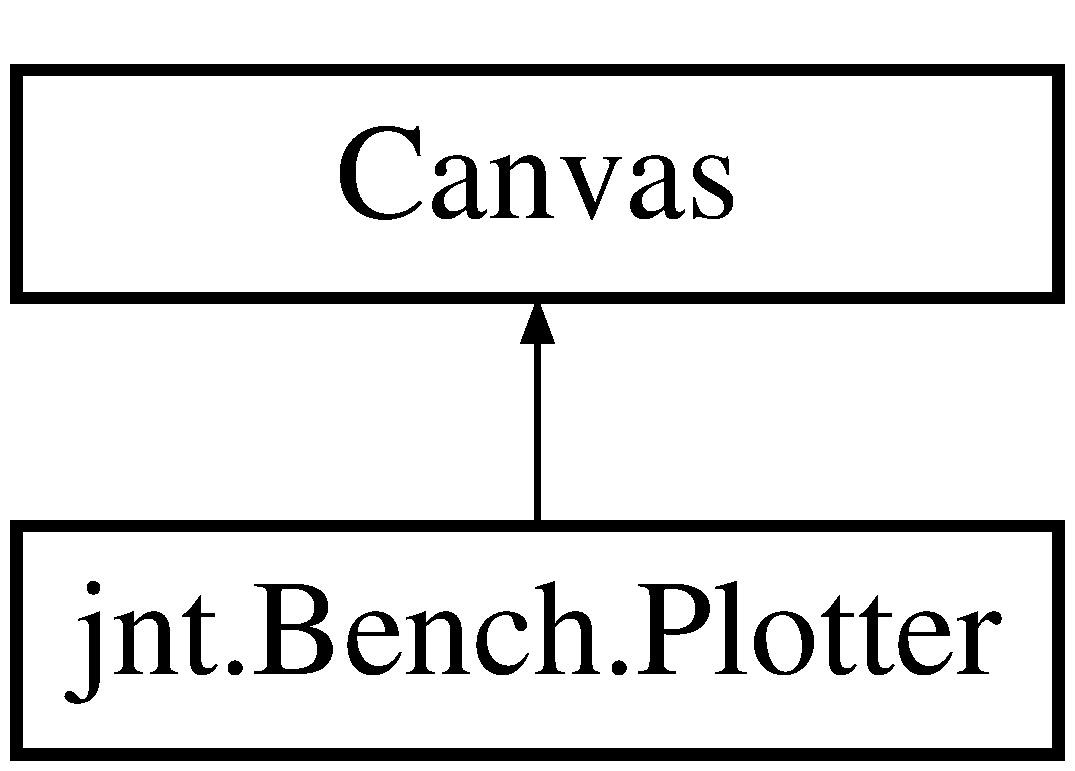
\includegraphics[height=2.000000cm]{da/d70/classjnt_1_1Bench_1_1Plotter}
\end{center}
\end{figure}
\subsection*{Fonctions membres publiques}
\begin{DoxyCompactItemize}
\item 
\hyperlink{classjnt_1_1Bench_1_1Plotter_aee05d05068e7384db48ca46263de6c0c}{Plotter} ()
\item 
void \hyperlink{classjnt_1_1Bench_1_1Plotter_a4da83c587691e9498053c2429f3fac56}{set\-Data} (String labels\mbox{[}$\,$\mbox{]}, double values\mbox{[}$\,$\mbox{]}, String axis\-Label, int specindex)
\item 
void \hyperlink{classjnt_1_1Bench_1_1Plotter_abff7e85d683ad0c694eb9deea523292e}{paint} (Graphics g)
\end{DoxyCompactItemize}


\subsection{Description détaillée}
\hyperlink{classjnt_1_1Bench_1_1Plotter}{Plotter} for the \hyperlink{classjnt_1_1Bench_1_1Bench}{Bench} Package Draws a horizontal bar graph, with labels for each bar at the left. A `\-Special' row, in a different color, is used to highlight the measurements of the current system.

\begin{DoxyAuthor}{Auteur}
Bruce R. Miller (\href{mailto:bruce.miller@nist.gov}{\tt bruce.\-miller@nist.\-gov}) 

Contribution of the National Institute of Standards and Technology, 

not subject to copyright. 
\end{DoxyAuthor}


\subsection{Documentation des constructeurs et destructeur}
\hypertarget{classjnt_1_1Bench_1_1Plotter_aee05d05068e7384db48ca46263de6c0c}{\index{jnt\-::\-Bench\-::\-Plotter@{jnt\-::\-Bench\-::\-Plotter}!Plotter@{Plotter}}
\index{Plotter@{Plotter}!jnt::Bench::Plotter@{jnt\-::\-Bench\-::\-Plotter}}
\subsubsection[{Plotter}]{\setlength{\rightskip}{0pt plus 5cm}jnt.\-Bench.\-Plotter.\-Plotter (
\begin{DoxyParamCaption}
{}
\end{DoxyParamCaption}
)}}\label{classjnt_1_1Bench_1_1Plotter_aee05d05068e7384db48ca46263de6c0c}


\subsection{Documentation des fonctions membres}
\hypertarget{classjnt_1_1Bench_1_1Plotter_abff7e85d683ad0c694eb9deea523292e}{\index{jnt\-::\-Bench\-::\-Plotter@{jnt\-::\-Bench\-::\-Plotter}!paint@{paint}}
\index{paint@{paint}!jnt::Bench::Plotter@{jnt\-::\-Bench\-::\-Plotter}}
\subsubsection[{paint}]{\setlength{\rightskip}{0pt plus 5cm}void jnt.\-Bench.\-Plotter.\-paint (
\begin{DoxyParamCaption}
\item[{Graphics}]{g}
\end{DoxyParamCaption}
)}}\label{classjnt_1_1Bench_1_1Plotter_abff7e85d683ad0c694eb9deea523292e}
\hypertarget{classjnt_1_1Bench_1_1Plotter_a4da83c587691e9498053c2429f3fac56}{\index{jnt\-::\-Bench\-::\-Plotter@{jnt\-::\-Bench\-::\-Plotter}!set\-Data@{set\-Data}}
\index{set\-Data@{set\-Data}!jnt::Bench::Plotter@{jnt\-::\-Bench\-::\-Plotter}}
\subsubsection[{set\-Data}]{\setlength{\rightskip}{0pt plus 5cm}void jnt.\-Bench.\-Plotter.\-set\-Data (
\begin{DoxyParamCaption}
\item[{String}]{labels\mbox{[}$\,$\mbox{]}, }
\item[{double}]{values\mbox{[}$\,$\mbox{]}, }
\item[{String}]{axis\-Label, }
\item[{int}]{specindex}
\end{DoxyParamCaption}
)}}\label{classjnt_1_1Bench_1_1Plotter_a4da83c587691e9498053c2429f3fac56}
Set the data to be displayed by the \hyperlink{classjnt_1_1Bench_1_1Plotter}{Plotter}. 
\begin{DoxyParams}{Paramètres}
{\em labels} & array of label strings for each bar. \\
\hline
{\em values} & array of values for the length of each bar. \\
\hline
{\em axis\-Label} & label for the X axis (along the bars). \\
\hline
{\em specindex} & the index of the `\-Special' entry. \\
\hline
\end{DoxyParams}


La documentation de cette classe a été générée à partir du fichier suivant \-:\begin{DoxyCompactItemize}
\item 
\hyperlink{Plotter_8java}{Plotter.\-java}\end{DoxyCompactItemize}

\hypertarget{classjnt_1_1scimark2_1_1Random}{\section{Référence de la classe jnt.\-scimark2.\-Random}
\label{classjnt_1_1scimark2_1_1Random}\index{jnt.\-scimark2.\-Random@{jnt.\-scimark2.\-Random}}
}
\subsection*{Fonctions membres publiques}
\begin{DoxyCompactItemize}
\item 
\hyperlink{classjnt_1_1scimark2_1_1Random_a3237e048e925076fefd7bec1c917e23e}{Random} ()
\item 
\hyperlink{classjnt_1_1scimark2_1_1Random_a11ce62c68016e6c84a9a70c63d3b3e4e}{Random} (double \hyperlink{classjnt_1_1scimark2_1_1Random_a3d63c681768d9fba34385c730b12de22}{left}, double \hyperlink{classjnt_1_1scimark2_1_1Random_a61abe62a2fb5de3294a2c231268bf893}{right})
\item 
\hyperlink{classjnt_1_1scimark2_1_1Random_ac13652259c67fcce72584f6b33fb88fc}{Random} (int seed)
\item 
\hyperlink{classjnt_1_1scimark2_1_1Random_a8f47099be80eae7ea808223f1fb75aa3}{Random} (int seed, double \hyperlink{classjnt_1_1scimark2_1_1Random_a3d63c681768d9fba34385c730b12de22}{left}, double \hyperlink{classjnt_1_1scimark2_1_1Random_a61abe62a2fb5de3294a2c231268bf893}{right})
\item 
final synchronized double \hyperlink{classjnt_1_1scimark2_1_1Random_a1a5cee3b6d5631f9922d89f96725cc9a}{next\-Double} ()
\item 
final synchronized void \hyperlink{classjnt_1_1scimark2_1_1Random_a61a639bf274d04604fcd78690e3b6eb0}{next\-Doubles} (double x\mbox{[}$\,$\mbox{]})
\end{DoxyCompactItemize}
\subsection*{Fonctions membres privées}
\begin{DoxyCompactItemize}
\item 
void \hyperlink{classjnt_1_1scimark2_1_1Random_ac62411f14367d260c01939f726f79630}{initialize} (int seed)
\end{DoxyCompactItemize}
\subsection*{Attributs privés}
\begin{DoxyCompactItemize}
\item 
int \hyperlink{classjnt_1_1scimark2_1_1Random_aed102d9fc6ee4e00f6ec50870b5ad88c}{m} \mbox{[}$\,$\mbox{]}
\item 
int \hyperlink{classjnt_1_1scimark2_1_1Random_a044347a46cf3161801a3739a2f249e66}{i} = 4
\item 
int \hyperlink{classjnt_1_1scimark2_1_1Random_a7d323c56dc4af7c9914e08175665cbcb}{j} = 16
\item 
final int \hyperlink{classjnt_1_1scimark2_1_1Random_ae9ade787ad441153ed665875e62030be}{mdig} = 32
\item 
final int \hyperlink{classjnt_1_1scimark2_1_1Random_a1d4281d838c46418fd2d30a4f1d52cf0}{one} = 1
\item 
final int \hyperlink{classjnt_1_1scimark2_1_1Random_ab7e096525b55f7e9368ba7aa4bffe41b}{m1} = (\hyperlink{classjnt_1_1scimark2_1_1Random_a1d4281d838c46418fd2d30a4f1d52cf0}{one} $<$$<$ \hyperlink{classjnt_1_1scimark2_1_1Random_ae9ade787ad441153ed665875e62030be}{mdig}-\/2) + ((\hyperlink{classjnt_1_1scimark2_1_1Random_a1d4281d838c46418fd2d30a4f1d52cf0}{one} $<$$<$ \hyperlink{classjnt_1_1scimark2_1_1Random_ae9ade787ad441153ed665875e62030be}{mdig}-\/2)-\/\hyperlink{classjnt_1_1scimark2_1_1Random_a1d4281d838c46418fd2d30a4f1d52cf0}{one})
\item 
final int \hyperlink{classjnt_1_1scimark2_1_1Random_a65a1436055bda1c6e25523e824e5373d}{m2} = \hyperlink{classjnt_1_1scimark2_1_1Random_a1d4281d838c46418fd2d30a4f1d52cf0}{one} $<$$<$ \hyperlink{classjnt_1_1scimark2_1_1Random_ae9ade787ad441153ed665875e62030be}{mdig}/2
\item 
double \hyperlink{classjnt_1_1scimark2_1_1Random_ad3888251b40ce8ae37a68b5b2e2bd0c5}{dm1} = 1.\-0 / (double) \hyperlink{classjnt_1_1scimark2_1_1Random_ab7e096525b55f7e9368ba7aa4bffe41b}{m1}
\item 
boolean \hyperlink{classjnt_1_1scimark2_1_1Random_a528187285b1330b8a017e2064118e868}{have\-Range} = false
\item 
double \hyperlink{classjnt_1_1scimark2_1_1Random_a3d63c681768d9fba34385c730b12de22}{left} = 0.\-0
\item 
double \hyperlink{classjnt_1_1scimark2_1_1Random_a61abe62a2fb5de3294a2c231268bf893}{right} = 1.\-0
\item 
double \hyperlink{classjnt_1_1scimark2_1_1Random_a9d0d92bf119171b4a77f7af5bd48693b}{width} = 1.\-0
\end{DoxyCompactItemize}


\subsection{Documentation des constructeurs et destructeur}
\hypertarget{classjnt_1_1scimark2_1_1Random_a3237e048e925076fefd7bec1c917e23e}{\index{jnt\-::scimark2\-::\-Random@{jnt\-::scimark2\-::\-Random}!Random@{Random}}
\index{Random@{Random}!jnt::scimark2::Random@{jnt\-::scimark2\-::\-Random}}
\subsubsection[{Random}]{\setlength{\rightskip}{0pt plus 5cm}jnt.\-scimark2.\-Random.\-Random (
\begin{DoxyParamCaption}
{}
\end{DoxyParamCaption}
)}}\label{classjnt_1_1scimark2_1_1Random_a3237e048e925076fefd7bec1c917e23e}
Initializes a sequence of uniformly distributed quasi random numbers with a seed based on the system clock. \hypertarget{classjnt_1_1scimark2_1_1Random_a11ce62c68016e6c84a9a70c63d3b3e4e}{\index{jnt\-::scimark2\-::\-Random@{jnt\-::scimark2\-::\-Random}!Random@{Random}}
\index{Random@{Random}!jnt::scimark2::Random@{jnt\-::scimark2\-::\-Random}}
\subsubsection[{Random}]{\setlength{\rightskip}{0pt plus 5cm}jnt.\-scimark2.\-Random.\-Random (
\begin{DoxyParamCaption}
\item[{double}]{left, }
\item[{double}]{right}
\end{DoxyParamCaption}
)}}\label{classjnt_1_1scimark2_1_1Random_a11ce62c68016e6c84a9a70c63d3b3e4e}
Initializes a sequence of uniformly distributed quasi random numbers on a given half-\/open interval \mbox{[}left,right) with a seed based on the system clock.


\begin{DoxyParams}{Paramètres}
{\em $<$\-B$>$left$<$/\-B$>$} & (double)\par
 \begin{DoxyVerb}   The left endpoint of the half-open interval [left,right).
\end{DoxyVerb}
\\
\hline
{\em $<$\-B$>$right$<$/\-B$>$} & (double)\par
 \begin{DoxyVerb}   The right endpoint of the half-open interval [left,right).\end{DoxyVerb}
 \\
\hline
\end{DoxyParams}
\hypertarget{classjnt_1_1scimark2_1_1Random_ac13652259c67fcce72584f6b33fb88fc}{\index{jnt\-::scimark2\-::\-Random@{jnt\-::scimark2\-::\-Random}!Random@{Random}}
\index{Random@{Random}!jnt::scimark2::Random@{jnt\-::scimark2\-::\-Random}}
\subsubsection[{Random}]{\setlength{\rightskip}{0pt plus 5cm}jnt.\-scimark2.\-Random.\-Random (
\begin{DoxyParamCaption}
\item[{int}]{seed}
\end{DoxyParamCaption}
)}}\label{classjnt_1_1scimark2_1_1Random_ac13652259c67fcce72584f6b33fb88fc}
Initializes a sequence of uniformly distributed quasi random numbers with a given seed.


\begin{DoxyParams}{Paramètres}
{\em $<$\-B$>$seed$<$/\-B$>$} & (int)\par
 \begin{DoxyVerb}   The seed of the random number generator.  Two sequences with the same
   seed will be identical.\end{DoxyVerb}
 \\
\hline
\end{DoxyParams}
\hypertarget{classjnt_1_1scimark2_1_1Random_a8f47099be80eae7ea808223f1fb75aa3}{\index{jnt\-::scimark2\-::\-Random@{jnt\-::scimark2\-::\-Random}!Random@{Random}}
\index{Random@{Random}!jnt::scimark2::Random@{jnt\-::scimark2\-::\-Random}}
\subsubsection[{Random}]{\setlength{\rightskip}{0pt plus 5cm}jnt.\-scimark2.\-Random.\-Random (
\begin{DoxyParamCaption}
\item[{int}]{seed, }
\item[{double}]{left, }
\item[{double}]{right}
\end{DoxyParamCaption}
)}}\label{classjnt_1_1scimark2_1_1Random_a8f47099be80eae7ea808223f1fb75aa3}
Initializes a sequence of uniformly distributed quasi random numbers with a given seed on a given half-\/open interval \mbox{[}left,right).


\begin{DoxyParams}{Paramètres}
{\em $<$\-B$>$seed$<$/\-B$>$} & (int)\par
 \begin{DoxyVerb}   The seed of the random number generator.  Two sequences with the same
   seed will be identical.
\end{DoxyVerb}
\\
\hline
{\em $<$\-B$>$left$<$/\-B$>$} & (double)\par
 \begin{DoxyVerb}   The left endpoint of the half-open interval [left,right).
\end{DoxyVerb}
\\
\hline
{\em $<$\-B$>$right$<$/\-B$>$} & (double)\par
 \begin{DoxyVerb}   The right endpoint of the half-open interval [left,right).\end{DoxyVerb}
 \\
\hline
\end{DoxyParams}


\subsection{Documentation des fonctions membres}
\hypertarget{classjnt_1_1scimark2_1_1Random_ac62411f14367d260c01939f726f79630}{\index{jnt\-::scimark2\-::\-Random@{jnt\-::scimark2\-::\-Random}!initialize@{initialize}}
\index{initialize@{initialize}!jnt::scimark2::Random@{jnt\-::scimark2\-::\-Random}}
\subsubsection[{initialize}]{\setlength{\rightskip}{0pt plus 5cm}void jnt.\-scimark2.\-Random.\-initialize (
\begin{DoxyParamCaption}
\item[{int}]{seed}
\end{DoxyParamCaption}
)\hspace{0.3cm}{\ttfamily [private]}}}\label{classjnt_1_1scimark2_1_1Random_ac62411f14367d260c01939f726f79630}
\hypertarget{classjnt_1_1scimark2_1_1Random_a1a5cee3b6d5631f9922d89f96725cc9a}{\index{jnt\-::scimark2\-::\-Random@{jnt\-::scimark2\-::\-Random}!next\-Double@{next\-Double}}
\index{next\-Double@{next\-Double}!jnt::scimark2::Random@{jnt\-::scimark2\-::\-Random}}
\subsubsection[{next\-Double}]{\setlength{\rightskip}{0pt plus 5cm}final synchronized double jnt.\-scimark2.\-Random.\-next\-Double (
\begin{DoxyParamCaption}
{}
\end{DoxyParamCaption}
)}}\label{classjnt_1_1scimark2_1_1Random_a1a5cee3b6d5631f9922d89f96725cc9a}
Returns the next random number in the sequence. \hypertarget{classjnt_1_1scimark2_1_1Random_a61a639bf274d04604fcd78690e3b6eb0}{\index{jnt\-::scimark2\-::\-Random@{jnt\-::scimark2\-::\-Random}!next\-Doubles@{next\-Doubles}}
\index{next\-Doubles@{next\-Doubles}!jnt::scimark2::Random@{jnt\-::scimark2\-::\-Random}}
\subsubsection[{next\-Doubles}]{\setlength{\rightskip}{0pt plus 5cm}final synchronized void jnt.\-scimark2.\-Random.\-next\-Doubles (
\begin{DoxyParamCaption}
\item[{double}]{x\mbox{[}$\,$\mbox{]}}
\end{DoxyParamCaption}
)}}\label{classjnt_1_1scimark2_1_1Random_a61a639bf274d04604fcd78690e3b6eb0}
Returns the next N random numbers in the sequence, as a vector. 

\subsection{Documentation des données membres}
\hypertarget{classjnt_1_1scimark2_1_1Random_ad3888251b40ce8ae37a68b5b2e2bd0c5}{\index{jnt\-::scimark2\-::\-Random@{jnt\-::scimark2\-::\-Random}!dm1@{dm1}}
\index{dm1@{dm1}!jnt::scimark2::Random@{jnt\-::scimark2\-::\-Random}}
\subsubsection[{dm1}]{\setlength{\rightskip}{0pt plus 5cm}double jnt.\-scimark2.\-Random.\-dm1 = 1.\-0 / (double) {\bf m1}\hspace{0.3cm}{\ttfamily [private]}}}\label{classjnt_1_1scimark2_1_1Random_ad3888251b40ce8ae37a68b5b2e2bd0c5}
\hypertarget{classjnt_1_1scimark2_1_1Random_a528187285b1330b8a017e2064118e868}{\index{jnt\-::scimark2\-::\-Random@{jnt\-::scimark2\-::\-Random}!have\-Range@{have\-Range}}
\index{have\-Range@{have\-Range}!jnt::scimark2::Random@{jnt\-::scimark2\-::\-Random}}
\subsubsection[{have\-Range}]{\setlength{\rightskip}{0pt plus 5cm}boolean jnt.\-scimark2.\-Random.\-have\-Range = false\hspace{0.3cm}{\ttfamily [private]}}}\label{classjnt_1_1scimark2_1_1Random_a528187285b1330b8a017e2064118e868}
\hypertarget{classjnt_1_1scimark2_1_1Random_a044347a46cf3161801a3739a2f249e66}{\index{jnt\-::scimark2\-::\-Random@{jnt\-::scimark2\-::\-Random}!i@{i}}
\index{i@{i}!jnt::scimark2::Random@{jnt\-::scimark2\-::\-Random}}
\subsubsection[{i}]{\setlength{\rightskip}{0pt plus 5cm}int jnt.\-scimark2.\-Random.\-i = 4\hspace{0.3cm}{\ttfamily [private]}}}\label{classjnt_1_1scimark2_1_1Random_a044347a46cf3161801a3739a2f249e66}
\hypertarget{classjnt_1_1scimark2_1_1Random_a7d323c56dc4af7c9914e08175665cbcb}{\index{jnt\-::scimark2\-::\-Random@{jnt\-::scimark2\-::\-Random}!j@{j}}
\index{j@{j}!jnt::scimark2::Random@{jnt\-::scimark2\-::\-Random}}
\subsubsection[{j}]{\setlength{\rightskip}{0pt plus 5cm}int jnt.\-scimark2.\-Random.\-j = 16\hspace{0.3cm}{\ttfamily [private]}}}\label{classjnt_1_1scimark2_1_1Random_a7d323c56dc4af7c9914e08175665cbcb}
\hypertarget{classjnt_1_1scimark2_1_1Random_a3d63c681768d9fba34385c730b12de22}{\index{jnt\-::scimark2\-::\-Random@{jnt\-::scimark2\-::\-Random}!left@{left}}
\index{left@{left}!jnt::scimark2::Random@{jnt\-::scimark2\-::\-Random}}
\subsubsection[{left}]{\setlength{\rightskip}{0pt plus 5cm}double jnt.\-scimark2.\-Random.\-left = 0.\-0\hspace{0.3cm}{\ttfamily [private]}}}\label{classjnt_1_1scimark2_1_1Random_a3d63c681768d9fba34385c730b12de22}
\hypertarget{classjnt_1_1scimark2_1_1Random_aed102d9fc6ee4e00f6ec50870b5ad88c}{\index{jnt\-::scimark2\-::\-Random@{jnt\-::scimark2\-::\-Random}!m@{m}}
\index{m@{m}!jnt::scimark2::Random@{jnt\-::scimark2\-::\-Random}}
\subsubsection[{m}]{\setlength{\rightskip}{0pt plus 5cm}int jnt.\-scimark2.\-Random.\-m\mbox{[}$\,$\mbox{]}\hspace{0.3cm}{\ttfamily [private]}}}\label{classjnt_1_1scimark2_1_1Random_aed102d9fc6ee4e00f6ec50870b5ad88c}
\hypertarget{classjnt_1_1scimark2_1_1Random_ab7e096525b55f7e9368ba7aa4bffe41b}{\index{jnt\-::scimark2\-::\-Random@{jnt\-::scimark2\-::\-Random}!m1@{m1}}
\index{m1@{m1}!jnt::scimark2::Random@{jnt\-::scimark2\-::\-Random}}
\subsubsection[{m1}]{\setlength{\rightskip}{0pt plus 5cm}final int jnt.\-scimark2.\-Random.\-m1 = ({\bf one} $<$$<$ {\bf mdig}-\/2) + (({\bf one} $<$$<$ {\bf mdig}-\/2)-\/{\bf one})\hspace{0.3cm}{\ttfamily [private]}}}\label{classjnt_1_1scimark2_1_1Random_ab7e096525b55f7e9368ba7aa4bffe41b}
\hypertarget{classjnt_1_1scimark2_1_1Random_a65a1436055bda1c6e25523e824e5373d}{\index{jnt\-::scimark2\-::\-Random@{jnt\-::scimark2\-::\-Random}!m2@{m2}}
\index{m2@{m2}!jnt::scimark2::Random@{jnt\-::scimark2\-::\-Random}}
\subsubsection[{m2}]{\setlength{\rightskip}{0pt plus 5cm}final int jnt.\-scimark2.\-Random.\-m2 = {\bf one} $<$$<$ {\bf mdig}/2\hspace{0.3cm}{\ttfamily [private]}}}\label{classjnt_1_1scimark2_1_1Random_a65a1436055bda1c6e25523e824e5373d}
\hypertarget{classjnt_1_1scimark2_1_1Random_ae9ade787ad441153ed665875e62030be}{\index{jnt\-::scimark2\-::\-Random@{jnt\-::scimark2\-::\-Random}!mdig@{mdig}}
\index{mdig@{mdig}!jnt::scimark2::Random@{jnt\-::scimark2\-::\-Random}}
\subsubsection[{mdig}]{\setlength{\rightskip}{0pt plus 5cm}final int jnt.\-scimark2.\-Random.\-mdig = 32\hspace{0.3cm}{\ttfamily [private]}}}\label{classjnt_1_1scimark2_1_1Random_ae9ade787ad441153ed665875e62030be}
\hypertarget{classjnt_1_1scimark2_1_1Random_a1d4281d838c46418fd2d30a4f1d52cf0}{\index{jnt\-::scimark2\-::\-Random@{jnt\-::scimark2\-::\-Random}!one@{one}}
\index{one@{one}!jnt::scimark2::Random@{jnt\-::scimark2\-::\-Random}}
\subsubsection[{one}]{\setlength{\rightskip}{0pt plus 5cm}final int jnt.\-scimark2.\-Random.\-one = 1\hspace{0.3cm}{\ttfamily [private]}}}\label{classjnt_1_1scimark2_1_1Random_a1d4281d838c46418fd2d30a4f1d52cf0}
\hypertarget{classjnt_1_1scimark2_1_1Random_a61abe62a2fb5de3294a2c231268bf893}{\index{jnt\-::scimark2\-::\-Random@{jnt\-::scimark2\-::\-Random}!right@{right}}
\index{right@{right}!jnt::scimark2::Random@{jnt\-::scimark2\-::\-Random}}
\subsubsection[{right}]{\setlength{\rightskip}{0pt plus 5cm}double jnt.\-scimark2.\-Random.\-right = 1.\-0\hspace{0.3cm}{\ttfamily [private]}}}\label{classjnt_1_1scimark2_1_1Random_a61abe62a2fb5de3294a2c231268bf893}
\hypertarget{classjnt_1_1scimark2_1_1Random_a9d0d92bf119171b4a77f7af5bd48693b}{\index{jnt\-::scimark2\-::\-Random@{jnt\-::scimark2\-::\-Random}!width@{width}}
\index{width@{width}!jnt::scimark2::Random@{jnt\-::scimark2\-::\-Random}}
\subsubsection[{width}]{\setlength{\rightskip}{0pt plus 5cm}double jnt.\-scimark2.\-Random.\-width = 1.\-0\hspace{0.3cm}{\ttfamily [private]}}}\label{classjnt_1_1scimark2_1_1Random_a9d0d92bf119171b4a77f7af5bd48693b}


La documentation de cette classe a été générée à partir du fichier suivant \-:\begin{DoxyCompactItemize}
\item 
\hyperlink{Random_8java}{Random.\-java}\end{DoxyCompactItemize}

\hypertarget{classjnt_1_1Bench_1_1SendMail}{\section{Référence de la classe jnt.\-Bench.\-Send\-Mail}
\label{classjnt_1_1Bench_1_1SendMail}\index{jnt.\-Bench.\-Send\-Mail@{jnt.\-Bench.\-Send\-Mail}}
}
\subsection*{Fonctions membres publiques statiques}
\begin{DoxyCompactItemize}
\item 
static void \hyperlink{classjnt_1_1Bench_1_1SendMail_a6514c64925df421389926727b16b40cf}{send} (String server, String sender, String recipient, String subject, String message)  throws Exception 
\end{DoxyCompactItemize}


\subsection{Description détaillée}
\hyperlink{classjnt_1_1Bench_1_1SendMail}{Send\-Mail} implements a simple S\-M\-T\-P client to send mail.

N\-O\-T\-E\-: Since a socket connection is used, when executed from an \hyperlink{classjnt_1_1Bench_1_1Applet}{Applet}, the security model requires that the server be the same as the server from which the applet was loaded.

\begin{DoxyAuthor}{Auteur}
Bruce R. Miller (\href{mailto:bruce.miller@nist.gov}{\tt bruce.\-miller@nist.\-gov}) 

Contribution of the National Institute of Standards and Technology, 

not subject to copyright. 
\end{DoxyAuthor}


\subsection{Documentation des fonctions membres}
\hypertarget{classjnt_1_1Bench_1_1SendMail_a6514c64925df421389926727b16b40cf}{\index{jnt\-::\-Bench\-::\-Send\-Mail@{jnt\-::\-Bench\-::\-Send\-Mail}!send@{send}}
\index{send@{send}!jnt::Bench::SendMail@{jnt\-::\-Bench\-::\-Send\-Mail}}
\subsubsection[{send}]{\setlength{\rightskip}{0pt plus 5cm}static void jnt.\-Bench.\-Send\-Mail.\-send (
\begin{DoxyParamCaption}
\item[{String}]{server, }
\item[{String}]{sender, }
\item[{String}]{recipient, }
\item[{String}]{subject, }
\item[{String}]{message}
\end{DoxyParamCaption}
) throws Exception\hspace{0.3cm}{\ttfamily [static]}}}\label{classjnt_1_1Bench_1_1SendMail_a6514c64925df421389926727b16b40cf}
Send an email message. 
\begin{DoxyParams}{Paramètres}
{\em server} & The S\-M\-T\-P server \\
\hline
{\em sender} & the sender's email address. \\
\hline
{\em recipient} & the recipient's email address. \\
\hline
{\em subject} & the subject of the message. \\
\hline
{\em the} & message text. \\
\hline
\end{DoxyParams}


La documentation de cette classe a été générée à partir du fichier suivant \-:\begin{DoxyCompactItemize}
\item 
\hyperlink{SendMail_8java}{Send\-Mail.\-java}\end{DoxyCompactItemize}

\hypertarget{classjnt_1_1BenchMarkResult_1_1SOR}{\section{Référence de la classe jnt.\-Bench\-Mark\-Result.\-S\-O\-R}
\label{classjnt_1_1BenchMarkResult_1_1SOR}\index{jnt.\-Bench\-Mark\-Result.\-S\-O\-R@{jnt.\-Bench\-Mark\-Result.\-S\-O\-R}}
}
\subsection*{Fonctions membres publiques}
\begin{DoxyCompactItemize}
\item 
\hyperlink{classjnt_1_1BenchMarkResult_1_1SOR_a78cbdd1234914949e07aff08c2ff9e03}{S\-O\-R} (int \hyperlink{classjnt_1_1BenchMarkResult_1_1SOR_ad3a37b811350f4fa2368a9a9973b8fb6}{size}, double \hyperlink{classjnt_1_1BenchMarkResult_1_1SOR_a607ca1495e3a8f4f92a550f415a9a96f}{value})
\end{DoxyCompactItemize}
\subsection*{Attributs publics}
\begin{DoxyCompactItemize}
\item 
int \hyperlink{classjnt_1_1BenchMarkResult_1_1SOR_ad3a37b811350f4fa2368a9a9973b8fb6}{size}
\item 
double \hyperlink{classjnt_1_1BenchMarkResult_1_1SOR_a607ca1495e3a8f4f92a550f415a9a96f}{value}
\end{DoxyCompactItemize}


\subsection{Description détaillée}
Classe contenant le résultat de la méthode de surrelaxation successive pour résoudre un système d'équations linéaires \begin{DoxySeeAlso}{Voir également}
\href{http://fr.wikipedia.org/wiki/M%C3%A9thode_de_surrelaxation_successive}{\tt Wikipedia} 
\end{DoxySeeAlso}
\begin{DoxyAuthor}{Auteur}

\begin{DoxyItemize}
\item Morgane Badré 
\item Vincent Wilmet 
\end{DoxyItemize}
\end{DoxyAuthor}
\begin{DoxyVersion}{Version}
1.\-0 
\end{DoxyVersion}


\subsection{Documentation des constructeurs et destructeur}
\hypertarget{classjnt_1_1BenchMarkResult_1_1SOR_a78cbdd1234914949e07aff08c2ff9e03}{\index{jnt\-::\-Bench\-Mark\-Result\-::\-S\-O\-R@{jnt\-::\-Bench\-Mark\-Result\-::\-S\-O\-R}!S\-O\-R@{S\-O\-R}}
\index{S\-O\-R@{S\-O\-R}!jnt::BenchMarkResult::SOR@{jnt\-::\-Bench\-Mark\-Result\-::\-S\-O\-R}}
\subsubsection[{S\-O\-R}]{\setlength{\rightskip}{0pt plus 5cm}jnt.\-Bench\-Mark\-Result.\-S\-O\-R.\-S\-O\-R (
\begin{DoxyParamCaption}
\item[{int}]{size, }
\item[{double}]{value}
\end{DoxyParamCaption}
)}}\label{classjnt_1_1BenchMarkResult_1_1SOR_a78cbdd1234914949e07aff08c2ff9e03}
Constructeur permettant d'initialiser les champs de la classe 
\begin{DoxyParams}{Paramètres}
{\em size} & La taille pour le calcul \\
\hline
{\em value} & La valeur \\
\hline
\end{DoxyParams}


\subsection{Documentation des données membres}
\hypertarget{classjnt_1_1BenchMarkResult_1_1SOR_ad3a37b811350f4fa2368a9a9973b8fb6}{\index{jnt\-::\-Bench\-Mark\-Result\-::\-S\-O\-R@{jnt\-::\-Bench\-Mark\-Result\-::\-S\-O\-R}!size@{size}}
\index{size@{size}!jnt::BenchMarkResult::SOR@{jnt\-::\-Bench\-Mark\-Result\-::\-S\-O\-R}}
\subsubsection[{size}]{\setlength{\rightskip}{0pt plus 5cm}int jnt.\-Bench\-Mark\-Result.\-S\-O\-R.\-size}}\label{classjnt_1_1BenchMarkResult_1_1SOR_ad3a37b811350f4fa2368a9a9973b8fb6}
Entier contenant la taille qui est necessaire pour le calcul \hypertarget{classjnt_1_1BenchMarkResult_1_1SOR_a607ca1495e3a8f4f92a550f415a9a96f}{\index{jnt\-::\-Bench\-Mark\-Result\-::\-S\-O\-R@{jnt\-::\-Bench\-Mark\-Result\-::\-S\-O\-R}!value@{value}}
\index{value@{value}!jnt::BenchMarkResult::SOR@{jnt\-::\-Bench\-Mark\-Result\-::\-S\-O\-R}}
\subsubsection[{value}]{\setlength{\rightskip}{0pt plus 5cm}double jnt.\-Bench\-Mark\-Result.\-S\-O\-R.\-value}}\label{classjnt_1_1BenchMarkResult_1_1SOR_a607ca1495e3a8f4f92a550f415a9a96f}
Réel contenant le résultat de ce calcul 

La documentation de cette classe a été générée à partir du fichier suivant \-:\begin{DoxyCompactItemize}
\item 
\hyperlink{BenchMarkResult_8java}{Bench\-Mark\-Result.\-java}\end{DoxyCompactItemize}

\hypertarget{classjnt_1_1scimark2_1_1SOR}{\section{Référence de la classe jnt.\-scimark2.\-S\-O\-R}
\label{classjnt_1_1scimark2_1_1SOR}\index{jnt.\-scimark2.\-S\-O\-R@{jnt.\-scimark2.\-S\-O\-R}}
}
\subsection*{Fonctions membres publiques statiques}
\begin{DoxyCompactItemize}
\item 
static final double \hyperlink{classjnt_1_1scimark2_1_1SOR_a0149ef2744ccc1d3d4804db67643583b}{num\-\_\-flops} (int M, int N, int num\-\_\-iterations)
\item 
static final void \hyperlink{classjnt_1_1scimark2_1_1SOR_aa52a59abae8229ff3552a1f6fb9c010e}{execute} (double omega, double G\mbox{[}$\,$\mbox{]}\mbox{[}$\,$\mbox{]}, int num\-\_\-iterations)
\end{DoxyCompactItemize}


\subsection{Documentation des fonctions membres}
\hypertarget{classjnt_1_1scimark2_1_1SOR_aa52a59abae8229ff3552a1f6fb9c010e}{\index{jnt\-::scimark2\-::\-S\-O\-R@{jnt\-::scimark2\-::\-S\-O\-R}!execute@{execute}}
\index{execute@{execute}!jnt::scimark2::SOR@{jnt\-::scimark2\-::\-S\-O\-R}}
\subsubsection[{execute}]{\setlength{\rightskip}{0pt plus 5cm}static final void jnt.\-scimark2.\-S\-O\-R.\-execute (
\begin{DoxyParamCaption}
\item[{double}]{omega, }
\item[{double}]{G\mbox{[}$\,$\mbox{]}\mbox{[}$\,$\mbox{]}, }
\item[{int}]{num\-\_\-iterations}
\end{DoxyParamCaption}
)\hspace{0.3cm}{\ttfamily [static]}}}\label{classjnt_1_1scimark2_1_1SOR_aa52a59abae8229ff3552a1f6fb9c010e}
\hypertarget{classjnt_1_1scimark2_1_1SOR_a0149ef2744ccc1d3d4804db67643583b}{\index{jnt\-::scimark2\-::\-S\-O\-R@{jnt\-::scimark2\-::\-S\-O\-R}!num\-\_\-flops@{num\-\_\-flops}}
\index{num\-\_\-flops@{num\-\_\-flops}!jnt::scimark2::SOR@{jnt\-::scimark2\-::\-S\-O\-R}}
\subsubsection[{num\-\_\-flops}]{\setlength{\rightskip}{0pt plus 5cm}static final double jnt.\-scimark2.\-S\-O\-R.\-num\-\_\-flops (
\begin{DoxyParamCaption}
\item[{int}]{M, }
\item[{int}]{N, }
\item[{int}]{num\-\_\-iterations}
\end{DoxyParamCaption}
)\hspace{0.3cm}{\ttfamily [static]}}}\label{classjnt_1_1scimark2_1_1SOR_a0149ef2744ccc1d3d4804db67643583b}


La documentation de cette classe a été générée à partir du fichier suivant \-:\begin{DoxyCompactItemize}
\item 
\hyperlink{SOR_8java}{S\-O\-R.\-java}\end{DoxyCompactItemize}

\hypertarget{classjnt_1_1scimark2_1_1SparseCompRow}{\section{Référence de la classe jnt.\-scimark2.\-Sparse\-Comp\-Row}
\label{classjnt_1_1scimark2_1_1SparseCompRow}\index{jnt.\-scimark2.\-Sparse\-Comp\-Row@{jnt.\-scimark2.\-Sparse\-Comp\-Row}}
}
\subsection*{Fonctions membres publiques statiques}
\begin{DoxyCompactItemize}
\item 
static double \hyperlink{classjnt_1_1scimark2_1_1SparseCompRow_a8728c9750af90bec93ce61aa5d9b304f}{num\-\_\-flops} (int N, int nz, int num\-\_\-iterations)
\item 
static void \hyperlink{classjnt_1_1scimark2_1_1SparseCompRow_ad63253daf63e9e95761838c6fc78b094}{matmult} (double y\mbox{[}$\,$\mbox{]}, double val\mbox{[}$\,$\mbox{]}, int row\mbox{[}$\,$\mbox{]}, int col\mbox{[}$\,$\mbox{]}, double x\mbox{[}$\,$\mbox{]}, int N\-U\-M\-\_\-\-I\-T\-E\-R\-A\-T\-I\-O\-N\-S)
\end{DoxyCompactItemize}


\subsection{Documentation des fonctions membres}
\hypertarget{classjnt_1_1scimark2_1_1SparseCompRow_ad63253daf63e9e95761838c6fc78b094}{\index{jnt\-::scimark2\-::\-Sparse\-Comp\-Row@{jnt\-::scimark2\-::\-Sparse\-Comp\-Row}!matmult@{matmult}}
\index{matmult@{matmult}!jnt::scimark2::SparseCompRow@{jnt\-::scimark2\-::\-Sparse\-Comp\-Row}}
\subsubsection[{matmult}]{\setlength{\rightskip}{0pt plus 5cm}static void jnt.\-scimark2.\-Sparse\-Comp\-Row.\-matmult (
\begin{DoxyParamCaption}
\item[{double}]{y\mbox{[}$\,$\mbox{]}, }
\item[{double}]{val\mbox{[}$\,$\mbox{]}, }
\item[{int}]{row\mbox{[}$\,$\mbox{]}, }
\item[{int}]{col\mbox{[}$\,$\mbox{]}, }
\item[{double}]{x\mbox{[}$\,$\mbox{]}, }
\item[{int}]{N\-U\-M\-\_\-\-I\-T\-E\-R\-A\-T\-I\-O\-N\-S}
\end{DoxyParamCaption}
)\hspace{0.3cm}{\ttfamily [static]}}}\label{classjnt_1_1scimark2_1_1SparseCompRow_ad63253daf63e9e95761838c6fc78b094}
\hypertarget{classjnt_1_1scimark2_1_1SparseCompRow_a8728c9750af90bec93ce61aa5d9b304f}{\index{jnt\-::scimark2\-::\-Sparse\-Comp\-Row@{jnt\-::scimark2\-::\-Sparse\-Comp\-Row}!num\-\_\-flops@{num\-\_\-flops}}
\index{num\-\_\-flops@{num\-\_\-flops}!jnt::scimark2::SparseCompRow@{jnt\-::scimark2\-::\-Sparse\-Comp\-Row}}
\subsubsection[{num\-\_\-flops}]{\setlength{\rightskip}{0pt plus 5cm}static double jnt.\-scimark2.\-Sparse\-Comp\-Row.\-num\-\_\-flops (
\begin{DoxyParamCaption}
\item[{int}]{N, }
\item[{int}]{nz, }
\item[{int}]{num\-\_\-iterations}
\end{DoxyParamCaption}
)\hspace{0.3cm}{\ttfamily [static]}}}\label{classjnt_1_1scimark2_1_1SparseCompRow_a8728c9750af90bec93ce61aa5d9b304f}


La documentation de cette classe a été générée à partir du fichier suivant \-:\begin{DoxyCompactItemize}
\item 
\hyperlink{SparseCompRow_8java}{Sparse\-Comp\-Row.\-java}\end{DoxyCompactItemize}

\hypertarget{classjnt_1_1BenchMarkResult_1_1SparseMatmult}{\section{Référence de la classe jnt.\-Bench\-Mark\-Result.\-Sparse\-Matmult}
\label{classjnt_1_1BenchMarkResult_1_1SparseMatmult}\index{jnt.\-Bench\-Mark\-Result.\-Sparse\-Matmult@{jnt.\-Bench\-Mark\-Result.\-Sparse\-Matmult}}
}
\subsection*{Fonctions membres publiques}
\begin{DoxyCompactItemize}
\item 
\hyperlink{classjnt_1_1BenchMarkResult_1_1SparseMatmult_ae40dc2e67e1e88d7daa0bd42db63c430}{Sparse\-Matmult} (int \hyperlink{classjnt_1_1BenchMarkResult_1_1SparseMatmult_a10bd94e346f3cf77c5a84fec1aa4a7d9}{size\-\_\-\-N}, int size\-\_\-nz, double \hyperlink{classjnt_1_1BenchMarkResult_1_1SparseMatmult_aa59accc2a3a250fcfbea547a16633082}{value})
\end{DoxyCompactItemize}
\subsection*{Attributs publics}
\begin{DoxyCompactItemize}
\item 
int \hyperlink{classjnt_1_1BenchMarkResult_1_1SparseMatmult_a10bd94e346f3cf77c5a84fec1aa4a7d9}{size\-\_\-\-N}
\item 
double \hyperlink{classjnt_1_1BenchMarkResult_1_1SparseMatmult_aa59accc2a3a250fcfbea547a16633082}{value}
\end{DoxyCompactItemize}


\subsection{Description détaillée}
Classe contenant le résultat de la multiplication de matrice vectoriel creuse \begin{DoxySeeAlso}{Voir également}
\href{http://www.cs.cmu.edu/~scandal/cacm/node9.html}{\tt Site Web} 
\end{DoxySeeAlso}
\begin{DoxyAuthor}{Auteur}

\begin{DoxyItemize}
\item Morgane Badré 
\item Vincent Wilmet 
\end{DoxyItemize}
\end{DoxyAuthor}
\begin{DoxyVersion}{Version}
1.\-0 
\end{DoxyVersion}


\subsection{Documentation des constructeurs et destructeur}
\hypertarget{classjnt_1_1BenchMarkResult_1_1SparseMatmult_ae40dc2e67e1e88d7daa0bd42db63c430}{\index{jnt\-::\-Bench\-Mark\-Result\-::\-Sparse\-Matmult@{jnt\-::\-Bench\-Mark\-Result\-::\-Sparse\-Matmult}!Sparse\-Matmult@{Sparse\-Matmult}}
\index{Sparse\-Matmult@{Sparse\-Matmult}!jnt::BenchMarkResult::SparseMatmult@{jnt\-::\-Bench\-Mark\-Result\-::\-Sparse\-Matmult}}
\subsubsection[{Sparse\-Matmult}]{\setlength{\rightskip}{0pt plus 5cm}jnt.\-Bench\-Mark\-Result.\-Sparse\-Matmult.\-Sparse\-Matmult (
\begin{DoxyParamCaption}
\item[{int}]{size\-\_\-\-N, }
\item[{int}]{size\-\_\-nz, }
\item[{double}]{value}
\end{DoxyParamCaption}
)}}\label{classjnt_1_1BenchMarkResult_1_1SparseMatmult_ae40dc2e67e1e88d7daa0bd42db63c430}
Constructeur permettant d'initialiser le champs de la classe 
\begin{DoxyParams}{Paramètres}
{\em value} & La valeur \\
\hline
{\em size\-\_\-\-N} & La taille N \\
\hline
{\em size\-\_\-nz} & La taille N\-Z \\
\hline
\end{DoxyParams}


\subsection{Documentation des données membres}
\hypertarget{classjnt_1_1BenchMarkResult_1_1SparseMatmult_a10bd94e346f3cf77c5a84fec1aa4a7d9}{\index{jnt\-::\-Bench\-Mark\-Result\-::\-Sparse\-Matmult@{jnt\-::\-Bench\-Mark\-Result\-::\-Sparse\-Matmult}!size\-\_\-\-N@{size\-\_\-\-N}}
\index{size\-\_\-\-N@{size\-\_\-\-N}!jnt::BenchMarkResult::SparseMatmult@{jnt\-::\-Bench\-Mark\-Result\-::\-Sparse\-Matmult}}
\subsubsection[{size\-\_\-\-N}]{\setlength{\rightskip}{0pt plus 5cm}int jnt.\-Bench\-Mark\-Result.\-Sparse\-Matmult.\-size\-\_\-\-N}}\label{classjnt_1_1BenchMarkResult_1_1SparseMatmult_a10bd94e346f3cf77c5a84fec1aa4a7d9}
Entiers contenant la taille qui est necessaire pour le calcul \hypertarget{classjnt_1_1BenchMarkResult_1_1SparseMatmult_aa59accc2a3a250fcfbea547a16633082}{\index{jnt\-::\-Bench\-Mark\-Result\-::\-Sparse\-Matmult@{jnt\-::\-Bench\-Mark\-Result\-::\-Sparse\-Matmult}!value@{value}}
\index{value@{value}!jnt::BenchMarkResult::SparseMatmult@{jnt\-::\-Bench\-Mark\-Result\-::\-Sparse\-Matmult}}
\subsubsection[{value}]{\setlength{\rightskip}{0pt plus 5cm}double jnt.\-Bench\-Mark\-Result.\-Sparse\-Matmult.\-value}}\label{classjnt_1_1BenchMarkResult_1_1SparseMatmult_aa59accc2a3a250fcfbea547a16633082}
Réel contenant le résultat de ce calcul 

La documentation de cette classe a été générée à partir du fichier suivant \-:\begin{DoxyCompactItemize}
\item 
\hyperlink{BenchMarkResult_8java}{Bench\-Mark\-Result.\-java}\end{DoxyCompactItemize}

\hypertarget{classjnt_1_1scimark2_1_1Stopwatch}{\section{Référence de la classe jnt.\-scimark2.\-Stopwatch}
\label{classjnt_1_1scimark2_1_1Stopwatch}\index{jnt.\-scimark2.\-Stopwatch@{jnt.\-scimark2.\-Stopwatch}}
}
\subsection*{Fonctions membres publiques}
\begin{DoxyCompactItemize}
\item 
void \hyperlink{classjnt_1_1scimark2_1_1Stopwatch_ac5442e147cb4734bb867cadeaf771cb4}{reset} ()
\item 
\hyperlink{classjnt_1_1scimark2_1_1Stopwatch_aab7050c4453e1d4578cf4e70aeddf231}{Stopwatch} ()
\item 
void \hyperlink{classjnt_1_1scimark2_1_1Stopwatch_abd9b30b3a0b8d81802aacc197a9d3237}{start} ()
\item 
void \hyperlink{classjnt_1_1scimark2_1_1Stopwatch_a6d1620c055cfb14c77aa0c559b3884bf}{resume} ()
\item 
double \hyperlink{classjnt_1_1scimark2_1_1Stopwatch_ab8958704af5479932936ba4d4fe552a1}{stop} ()
\item 
double \hyperlink{classjnt_1_1scimark2_1_1Stopwatch_a8788eccb2ccec8c62aafbf8fb1eae416}{read} ()
\end{DoxyCompactItemize}
\subsection*{Fonctions membres publiques statiques}
\begin{DoxyCompactItemize}
\item 
static final double \hyperlink{classjnt_1_1scimark2_1_1Stopwatch_ab504eef5baa37fe4d90d530623adcf40}{seconds} ()
\end{DoxyCompactItemize}
\subsection*{Attributs privés}
\begin{DoxyCompactItemize}
\item 
boolean \hyperlink{classjnt_1_1scimark2_1_1Stopwatch_a8c263f03c85291abc4d4e9c32a0083b3}{running}
\item 
double \hyperlink{classjnt_1_1scimark2_1_1Stopwatch_a73fc2c69e2ed31f72dd55ef03ef58576}{last\-\_\-time}
\item 
double \hyperlink{classjnt_1_1scimark2_1_1Stopwatch_ae3a413a0f9c0fab717d98fa5af2bcabb}{total}
\end{DoxyCompactItemize}


\subsection{Description détaillée}
Provides a stopwatch to measure elapsed time.


\begin{DoxyDescription}
\item[{\bfseries Example of use\-:} ]


\begin{DoxyPre}
      \hyperlink{classjnt_1_1scimark2_1_1Stopwatch}{Stopwatch} Q = new \hyperlink{classjnt_1_1scimark2_1_1Stopwatch}{Stopwatch};
\end{DoxyPre}



\begin{DoxyPre}
      Q.start();
      //
      // code to be timed here ...
      //
      Q.stop();
      System.out.println("elapsed time was: " + Q.read() + " seconds.");
\end{DoxyPre}


\begin{DoxyAuthor}{Auteur}
Roldan Pozo 
\end{DoxyAuthor}
\begin{DoxyVersion}{Version}
14 October 1997, revised 1999-\/04-\/24 
\end{DoxyVersion}

\end{DoxyDescription}

\subsection{Documentation des constructeurs et destructeur}
\hypertarget{classjnt_1_1scimark2_1_1Stopwatch_aab7050c4453e1d4578cf4e70aeddf231}{\index{jnt\-::scimark2\-::\-Stopwatch@{jnt\-::scimark2\-::\-Stopwatch}!Stopwatch@{Stopwatch}}
\index{Stopwatch@{Stopwatch}!jnt::scimark2::Stopwatch@{jnt\-::scimark2\-::\-Stopwatch}}
\subsubsection[{Stopwatch}]{\setlength{\rightskip}{0pt plus 5cm}jnt.\-scimark2.\-Stopwatch.\-Stopwatch (
\begin{DoxyParamCaption}
{}
\end{DoxyParamCaption}
)}}\label{classjnt_1_1scimark2_1_1Stopwatch_aab7050c4453e1d4578cf4e70aeddf231}


\subsection{Documentation des fonctions membres}
\hypertarget{classjnt_1_1scimark2_1_1Stopwatch_a8788eccb2ccec8c62aafbf8fb1eae416}{\index{jnt\-::scimark2\-::\-Stopwatch@{jnt\-::scimark2\-::\-Stopwatch}!read@{read}}
\index{read@{read}!jnt::scimark2::Stopwatch@{jnt\-::scimark2\-::\-Stopwatch}}
\subsubsection[{read}]{\setlength{\rightskip}{0pt plus 5cm}double jnt.\-scimark2.\-Stopwatch.\-read (
\begin{DoxyParamCaption}
{}
\end{DoxyParamCaption}
)}}\label{classjnt_1_1scimark2_1_1Stopwatch_a8788eccb2ccec8c62aafbf8fb1eae416}
Display the elapsed time (in seconds) \hypertarget{classjnt_1_1scimark2_1_1Stopwatch_ac5442e147cb4734bb867cadeaf771cb4}{\index{jnt\-::scimark2\-::\-Stopwatch@{jnt\-::scimark2\-::\-Stopwatch}!reset@{reset}}
\index{reset@{reset}!jnt::scimark2::Stopwatch@{jnt\-::scimark2\-::\-Stopwatch}}
\subsubsection[{reset}]{\setlength{\rightskip}{0pt plus 5cm}void jnt.\-scimark2.\-Stopwatch.\-reset (
\begin{DoxyParamCaption}
{}
\end{DoxyParamCaption}
)}}\label{classjnt_1_1scimark2_1_1Stopwatch_ac5442e147cb4734bb867cadeaf771cb4}
Return system time (in seconds) \hypertarget{classjnt_1_1scimark2_1_1Stopwatch_a6d1620c055cfb14c77aa0c559b3884bf}{\index{jnt\-::scimark2\-::\-Stopwatch@{jnt\-::scimark2\-::\-Stopwatch}!resume@{resume}}
\index{resume@{resume}!jnt::scimark2::Stopwatch@{jnt\-::scimark2\-::\-Stopwatch}}
\subsubsection[{resume}]{\setlength{\rightskip}{0pt plus 5cm}void jnt.\-scimark2.\-Stopwatch.\-resume (
\begin{DoxyParamCaption}
{}
\end{DoxyParamCaption}
)}}\label{classjnt_1_1scimark2_1_1Stopwatch_a6d1620c055cfb14c77aa0c559b3884bf}
Resume timing, after stopping. (Does not wipe out accumulated times.) \hypertarget{classjnt_1_1scimark2_1_1Stopwatch_ab504eef5baa37fe4d90d530623adcf40}{\index{jnt\-::scimark2\-::\-Stopwatch@{jnt\-::scimark2\-::\-Stopwatch}!seconds@{seconds}}
\index{seconds@{seconds}!jnt::scimark2::Stopwatch@{jnt\-::scimark2\-::\-Stopwatch}}
\subsubsection[{seconds}]{\setlength{\rightskip}{0pt plus 5cm}static final double jnt.\-scimark2.\-Stopwatch.\-seconds (
\begin{DoxyParamCaption}
{}
\end{DoxyParamCaption}
)\hspace{0.3cm}{\ttfamily [static]}}}\label{classjnt_1_1scimark2_1_1Stopwatch_ab504eef5baa37fe4d90d530623adcf40}
Return system time (in seconds) \hypertarget{classjnt_1_1scimark2_1_1Stopwatch_abd9b30b3a0b8d81802aacc197a9d3237}{\index{jnt\-::scimark2\-::\-Stopwatch@{jnt\-::scimark2\-::\-Stopwatch}!start@{start}}
\index{start@{start}!jnt::scimark2::Stopwatch@{jnt\-::scimark2\-::\-Stopwatch}}
\subsubsection[{start}]{\setlength{\rightskip}{0pt plus 5cm}void jnt.\-scimark2.\-Stopwatch.\-start (
\begin{DoxyParamCaption}
{}
\end{DoxyParamCaption}
)}}\label{classjnt_1_1scimark2_1_1Stopwatch_abd9b30b3a0b8d81802aacc197a9d3237}
Start (and reset) timer \hypertarget{classjnt_1_1scimark2_1_1Stopwatch_ab8958704af5479932936ba4d4fe552a1}{\index{jnt\-::scimark2\-::\-Stopwatch@{jnt\-::scimark2\-::\-Stopwatch}!stop@{stop}}
\index{stop@{stop}!jnt::scimark2::Stopwatch@{jnt\-::scimark2\-::\-Stopwatch}}
\subsubsection[{stop}]{\setlength{\rightskip}{0pt plus 5cm}double jnt.\-scimark2.\-Stopwatch.\-stop (
\begin{DoxyParamCaption}
{}
\end{DoxyParamCaption}
)}}\label{classjnt_1_1scimark2_1_1Stopwatch_ab8958704af5479932936ba4d4fe552a1}
Stop timer 

\subsection{Documentation des données membres}
\hypertarget{classjnt_1_1scimark2_1_1Stopwatch_a73fc2c69e2ed31f72dd55ef03ef58576}{\index{jnt\-::scimark2\-::\-Stopwatch@{jnt\-::scimark2\-::\-Stopwatch}!last\-\_\-time@{last\-\_\-time}}
\index{last\-\_\-time@{last\-\_\-time}!jnt::scimark2::Stopwatch@{jnt\-::scimark2\-::\-Stopwatch}}
\subsubsection[{last\-\_\-time}]{\setlength{\rightskip}{0pt plus 5cm}double jnt.\-scimark2.\-Stopwatch.\-last\-\_\-time\hspace{0.3cm}{\ttfamily [private]}}}\label{classjnt_1_1scimark2_1_1Stopwatch_a73fc2c69e2ed31f72dd55ef03ef58576}
\hypertarget{classjnt_1_1scimark2_1_1Stopwatch_a8c263f03c85291abc4d4e9c32a0083b3}{\index{jnt\-::scimark2\-::\-Stopwatch@{jnt\-::scimark2\-::\-Stopwatch}!running@{running}}
\index{running@{running}!jnt::scimark2::Stopwatch@{jnt\-::scimark2\-::\-Stopwatch}}
\subsubsection[{running}]{\setlength{\rightskip}{0pt plus 5cm}boolean jnt.\-scimark2.\-Stopwatch.\-running\hspace{0.3cm}{\ttfamily [private]}}}\label{classjnt_1_1scimark2_1_1Stopwatch_a8c263f03c85291abc4d4e9c32a0083b3}
\hypertarget{classjnt_1_1scimark2_1_1Stopwatch_ae3a413a0f9c0fab717d98fa5af2bcabb}{\index{jnt\-::scimark2\-::\-Stopwatch@{jnt\-::scimark2\-::\-Stopwatch}!total@{total}}
\index{total@{total}!jnt::scimark2::Stopwatch@{jnt\-::scimark2\-::\-Stopwatch}}
\subsubsection[{total}]{\setlength{\rightskip}{0pt plus 5cm}double jnt.\-scimark2.\-Stopwatch.\-total\hspace{0.3cm}{\ttfamily [private]}}}\label{classjnt_1_1scimark2_1_1Stopwatch_ae3a413a0f9c0fab717d98fa5af2bcabb}


La documentation de cette classe a été générée à partir du fichier suivant \-:\begin{DoxyCompactItemize}
\item 
\hyperlink{scimark2_2Stopwatch_8java}{scimark2/\-Stopwatch.\-java}\end{DoxyCompactItemize}

\hypertarget{classjnt_1_1Bench_1_1Stopwatch}{\section{Référence de la classe jnt.\-Bench.\-Stopwatch}
\label{classjnt_1_1Bench_1_1Stopwatch}\index{jnt.\-Bench.\-Stopwatch@{jnt.\-Bench.\-Stopwatch}}
}
\subsection*{Fonctions membres publiques}
\begin{DoxyCompactItemize}
\item 
\hyperlink{classjnt_1_1Bench_1_1Stopwatch_aa6504215d7507057731bac58d84b392f}{Stopwatch} ()
\item 
void \hyperlink{classjnt_1_1Bench_1_1Stopwatch_a3caeba308010905f2705b7d4f66cf55f}{reset} ()
\item 
void \hyperlink{classjnt_1_1Bench_1_1Stopwatch_a9bac3f537a5ef70c09530483e4384b50}{resume} ()
\item 
void \hyperlink{classjnt_1_1Bench_1_1Stopwatch_a2449b37f8bead3218c6d912b03a5c034}{start} ()
\item 
double \hyperlink{classjnt_1_1Bench_1_1Stopwatch_a2138dc3daabedc78480f3f6434673c89}{stop} ()
\item 
double \hyperlink{classjnt_1_1Bench_1_1Stopwatch_a60efa1d72bd5eb1df41b77480a833df7}{read} ()
\end{DoxyCompactItemize}
\subsection*{Attributs privés}
\begin{DoxyCompactItemize}
\item 
boolean \hyperlink{classjnt_1_1Bench_1_1Stopwatch_aa0a2a8cae25b4860113e0f89ff7d01b5}{running}
\item 
long \hyperlink{classjnt_1_1Bench_1_1Stopwatch_a886c0806e96b71415c5911dad7380206}{last\-\_\-time}
\item 
long \hyperlink{classjnt_1_1Bench_1_1Stopwatch_a3c184cc059a96f96394d3520fbd20599}{total}
\end{DoxyCompactItemize}


\subsection{Description détaillée}
Provides a stopwatch to measure elapsed time. 
\begin{DoxyDescription}
\item[{\bfseries Example of use\-:} ]
\begin{DoxyPre}
      \hyperlink{classjnt_1_1Bench_1_1Stopwatch}{Stopwatch} Q = new \hyperlink{classjnt_1_1Bench_1_1Stopwatch}{Stopwatch};
      Q.start();
      //
      // code to be timed here ...
      //
      Q.stop();
      System.out.println("elapsed time was: " + Q.read() + " seconds.");
\end{DoxyPre}


\begin{DoxyAuthor}{Auteur}
Roldan Pozo 
\end{DoxyAuthor}
\begin{DoxyVersion}{Version}
14 October 1997 
\end{DoxyVersion}

\end{DoxyDescription}

\subsection{Documentation des constructeurs et destructeur}
\hypertarget{classjnt_1_1Bench_1_1Stopwatch_aa6504215d7507057731bac58d84b392f}{\index{jnt\-::\-Bench\-::\-Stopwatch@{jnt\-::\-Bench\-::\-Stopwatch}!Stopwatch@{Stopwatch}}
\index{Stopwatch@{Stopwatch}!jnt::Bench::Stopwatch@{jnt\-::\-Bench\-::\-Stopwatch}}
\subsubsection[{Stopwatch}]{\setlength{\rightskip}{0pt plus 5cm}jnt.\-Bench.\-Stopwatch.\-Stopwatch (
\begin{DoxyParamCaption}
{}
\end{DoxyParamCaption}
)}}\label{classjnt_1_1Bench_1_1Stopwatch_aa6504215d7507057731bac58d84b392f}


\subsection{Documentation des fonctions membres}
\hypertarget{classjnt_1_1Bench_1_1Stopwatch_a60efa1d72bd5eb1df41b77480a833df7}{\index{jnt\-::\-Bench\-::\-Stopwatch@{jnt\-::\-Bench\-::\-Stopwatch}!read@{read}}
\index{read@{read}!jnt::Bench::Stopwatch@{jnt\-::\-Bench\-::\-Stopwatch}}
\subsubsection[{read}]{\setlength{\rightskip}{0pt plus 5cm}double jnt.\-Bench.\-Stopwatch.\-read (
\begin{DoxyParamCaption}
{}
\end{DoxyParamCaption}
)}}\label{classjnt_1_1Bench_1_1Stopwatch_a60efa1d72bd5eb1df41b77480a833df7}
Return the elapsed time (in seconds) \hypertarget{classjnt_1_1Bench_1_1Stopwatch_a3caeba308010905f2705b7d4f66cf55f}{\index{jnt\-::\-Bench\-::\-Stopwatch@{jnt\-::\-Bench\-::\-Stopwatch}!reset@{reset}}
\index{reset@{reset}!jnt::Bench::Stopwatch@{jnt\-::\-Bench\-::\-Stopwatch}}
\subsubsection[{reset}]{\setlength{\rightskip}{0pt plus 5cm}void jnt.\-Bench.\-Stopwatch.\-reset (
\begin{DoxyParamCaption}
{}
\end{DoxyParamCaption}
)}}\label{classjnt_1_1Bench_1_1Stopwatch_a3caeba308010905f2705b7d4f66cf55f}
Return system time (in seconds) \hypertarget{classjnt_1_1Bench_1_1Stopwatch_a9bac3f537a5ef70c09530483e4384b50}{\index{jnt\-::\-Bench\-::\-Stopwatch@{jnt\-::\-Bench\-::\-Stopwatch}!resume@{resume}}
\index{resume@{resume}!jnt::Bench::Stopwatch@{jnt\-::\-Bench\-::\-Stopwatch}}
\subsubsection[{resume}]{\setlength{\rightskip}{0pt plus 5cm}void jnt.\-Bench.\-Stopwatch.\-resume (
\begin{DoxyParamCaption}
{}
\end{DoxyParamCaption}
)}}\label{classjnt_1_1Bench_1_1Stopwatch_a9bac3f537a5ef70c09530483e4384b50}
Resume timer. \hypertarget{classjnt_1_1Bench_1_1Stopwatch_a2449b37f8bead3218c6d912b03a5c034}{\index{jnt\-::\-Bench\-::\-Stopwatch@{jnt\-::\-Bench\-::\-Stopwatch}!start@{start}}
\index{start@{start}!jnt::Bench::Stopwatch@{jnt\-::\-Bench\-::\-Stopwatch}}
\subsubsection[{start}]{\setlength{\rightskip}{0pt plus 5cm}void jnt.\-Bench.\-Stopwatch.\-start (
\begin{DoxyParamCaption}
{}
\end{DoxyParamCaption}
)}}\label{classjnt_1_1Bench_1_1Stopwatch_a2449b37f8bead3218c6d912b03a5c034}
Start (and reset) timer \hypertarget{classjnt_1_1Bench_1_1Stopwatch_a2138dc3daabedc78480f3f6434673c89}{\index{jnt\-::\-Bench\-::\-Stopwatch@{jnt\-::\-Bench\-::\-Stopwatch}!stop@{stop}}
\index{stop@{stop}!jnt::Bench::Stopwatch@{jnt\-::\-Bench\-::\-Stopwatch}}
\subsubsection[{stop}]{\setlength{\rightskip}{0pt plus 5cm}double jnt.\-Bench.\-Stopwatch.\-stop (
\begin{DoxyParamCaption}
{}
\end{DoxyParamCaption}
)}}\label{classjnt_1_1Bench_1_1Stopwatch_a2138dc3daabedc78480f3f6434673c89}
Stop timer 

\subsection{Documentation des données membres}
\hypertarget{classjnt_1_1Bench_1_1Stopwatch_a886c0806e96b71415c5911dad7380206}{\index{jnt\-::\-Bench\-::\-Stopwatch@{jnt\-::\-Bench\-::\-Stopwatch}!last\-\_\-time@{last\-\_\-time}}
\index{last\-\_\-time@{last\-\_\-time}!jnt::Bench::Stopwatch@{jnt\-::\-Bench\-::\-Stopwatch}}
\subsubsection[{last\-\_\-time}]{\setlength{\rightskip}{0pt plus 5cm}long jnt.\-Bench.\-Stopwatch.\-last\-\_\-time\hspace{0.3cm}{\ttfamily [private]}}}\label{classjnt_1_1Bench_1_1Stopwatch_a886c0806e96b71415c5911dad7380206}
\hypertarget{classjnt_1_1Bench_1_1Stopwatch_aa0a2a8cae25b4860113e0f89ff7d01b5}{\index{jnt\-::\-Bench\-::\-Stopwatch@{jnt\-::\-Bench\-::\-Stopwatch}!running@{running}}
\index{running@{running}!jnt::Bench::Stopwatch@{jnt\-::\-Bench\-::\-Stopwatch}}
\subsubsection[{running}]{\setlength{\rightskip}{0pt plus 5cm}boolean jnt.\-Bench.\-Stopwatch.\-running\hspace{0.3cm}{\ttfamily [private]}}}\label{classjnt_1_1Bench_1_1Stopwatch_aa0a2a8cae25b4860113e0f89ff7d01b5}
\hypertarget{classjnt_1_1Bench_1_1Stopwatch_a3c184cc059a96f96394d3520fbd20599}{\index{jnt\-::\-Bench\-::\-Stopwatch@{jnt\-::\-Bench\-::\-Stopwatch}!total@{total}}
\index{total@{total}!jnt::Bench::Stopwatch@{jnt\-::\-Bench\-::\-Stopwatch}}
\subsubsection[{total}]{\setlength{\rightskip}{0pt plus 5cm}long jnt.\-Bench.\-Stopwatch.\-total\hspace{0.3cm}{\ttfamily [private]}}}\label{classjnt_1_1Bench_1_1Stopwatch_a3c184cc059a96f96394d3520fbd20599}


La documentation de cette classe a été générée à partir du fichier suivant \-:\begin{DoxyCompactItemize}
\item 
\hyperlink{Bench_2Stopwatch_8java}{Bench/\-Stopwatch.\-java}\end{DoxyCompactItemize}

\hypertarget{classjnt_1_1Bench_1_1SubmitDialog}{\section{Référence de la classe jnt.\-Bench.\-Submit\-Dialog}
\label{classjnt_1_1Bench_1_1SubmitDialog}\index{jnt.\-Bench.\-Submit\-Dialog@{jnt.\-Bench.\-Submit\-Dialog}}
}
Graphe d'héritage de jnt.\-Bench.\-Submit\-Dialog\-:\begin{figure}[H]
\begin{center}
\leavevmode
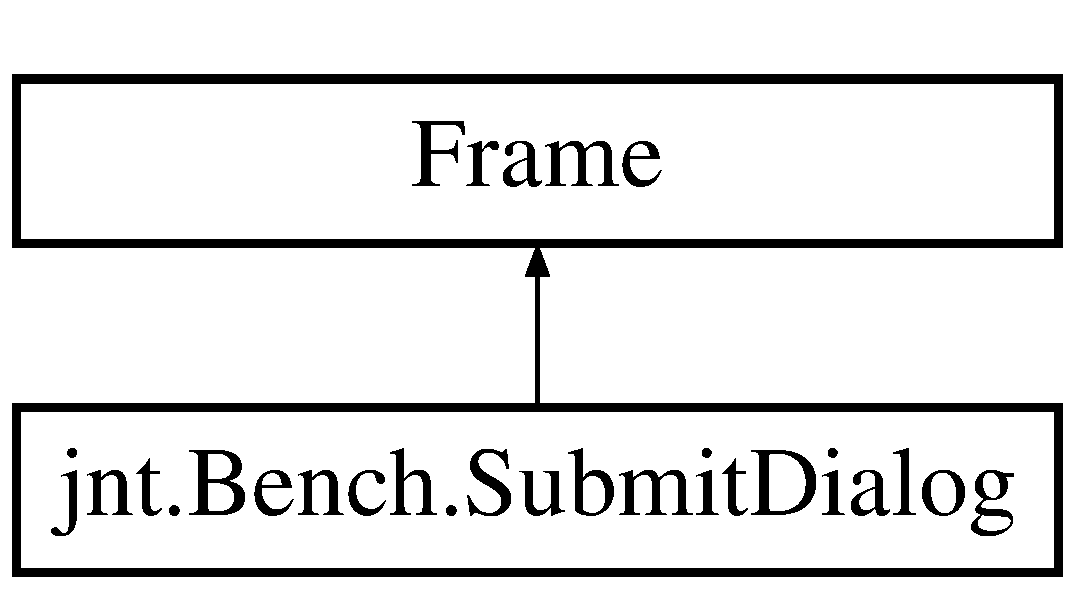
\includegraphics[height=2.000000cm]{d0/da7/classjnt_1_1Bench_1_1SubmitDialog}
\end{center}
\end{figure}
\subsection*{Fonctions membres publiques}
\begin{DoxyCompactItemize}
\item 
\hyperlink{classjnt_1_1Bench_1_1SubmitDialog_ac6dc8de0e644ad60f8f5faf4e91b2837}{Submit\-Dialog} (\hyperlink{classjnt_1_1Bench_1_1Applet}{Applet} applet, \hyperlink{classjnt_1_1Bench_1_1Bench}{Bench} bench)
\item 
boolean \hyperlink{classjnt_1_1Bench_1_1SubmitDialog_a27946c9f56eab29a4fb8695e485e71f6}{handle\-Event} (Event e)
\end{DoxyCompactItemize}


\subsection{Description détaillée}
\hyperlink{classjnt_1_1Bench_1_1SubmitDialog}{Submit\-Dialog} provides a Dialog box for filling in a benchmark submission. It extracts the relevent information from System.\-Properties of the V\-M, and provides text boxes for filling in other information. It uses \hyperlink{classjnt_1_1Bench_1_1SendMail}{Bench.\-Send\-Mail} to send the message, and uses callbacks to the \hyperlink{classjnt_1_1Bench_1_1Applet}{Applet} (if any) to inform of the success or failure of the submission. 

\subsection{Documentation des constructeurs et destructeur}
\hypertarget{classjnt_1_1Bench_1_1SubmitDialog_ac6dc8de0e644ad60f8f5faf4e91b2837}{\index{jnt\-::\-Bench\-::\-Submit\-Dialog@{jnt\-::\-Bench\-::\-Submit\-Dialog}!Submit\-Dialog@{Submit\-Dialog}}
\index{Submit\-Dialog@{Submit\-Dialog}!jnt::Bench::SubmitDialog@{jnt\-::\-Bench\-::\-Submit\-Dialog}}
\subsubsection[{Submit\-Dialog}]{\setlength{\rightskip}{0pt plus 5cm}jnt.\-Bench.\-Submit\-Dialog.\-Submit\-Dialog (
\begin{DoxyParamCaption}
\item[{{\bf Applet}}]{applet, }
\item[{{\bf Bench}}]{bench}
\end{DoxyParamCaption}
)}}\label{classjnt_1_1Bench_1_1SubmitDialog_ac6dc8de0e644ad60f8f5faf4e91b2837}
Create a \hyperlink{classjnt_1_1Bench_1_1SubmitDialog}{Submit\-Dialog} to report on a new measurement of the Benchmark \hyperlink{interfacejnt_1_1Bench_1_1Target}{Target} described in bench. 

\subsection{Documentation des fonctions membres}
\hypertarget{classjnt_1_1Bench_1_1SubmitDialog_a27946c9f56eab29a4fb8695e485e71f6}{\index{jnt\-::\-Bench\-::\-Submit\-Dialog@{jnt\-::\-Bench\-::\-Submit\-Dialog}!handle\-Event@{handle\-Event}}
\index{handle\-Event@{handle\-Event}!jnt::Bench::SubmitDialog@{jnt\-::\-Bench\-::\-Submit\-Dialog}}
\subsubsection[{handle\-Event}]{\setlength{\rightskip}{0pt plus 5cm}boolean jnt.\-Bench.\-Submit\-Dialog.\-handle\-Event (
\begin{DoxyParamCaption}
\item[{Event}]{e}
\end{DoxyParamCaption}
)}}\label{classjnt_1_1Bench_1_1SubmitDialog_a27946c9f56eab29a4fb8695e485e71f6}


La documentation de cette classe a été générée à partir du fichier suivant \-:\begin{DoxyCompactItemize}
\item 
\hyperlink{SubmitDialog_8java}{Submit\-Dialog.\-java}\end{DoxyCompactItemize}

\hypertarget{interfacejnt_1_1Bench_1_1Target}{\section{Référence de l'interface jnt.\-Bench.\-Target}
\label{interfacejnt_1_1Bench_1_1Target}\index{jnt.\-Bench.\-Target@{jnt.\-Bench.\-Target}}
}
Graphe d'héritage de jnt.\-Bench.\-Target\-:\begin{figure}[H]
\begin{center}
\leavevmode
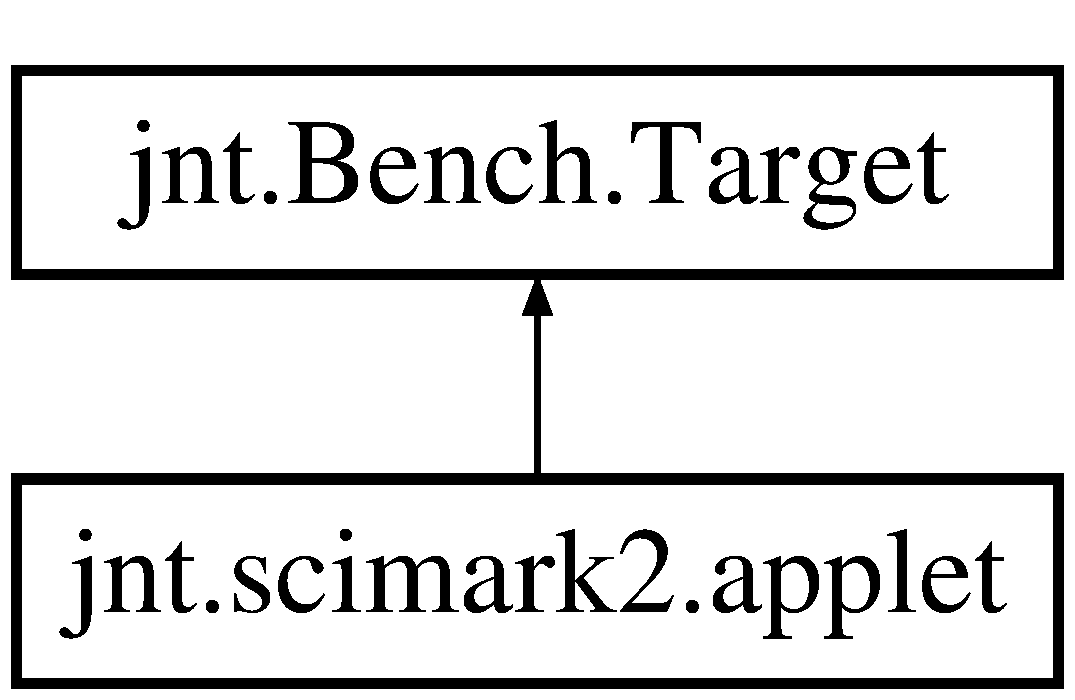
\includegraphics[height=2.000000cm]{de/d37/interfacejnt_1_1Bench_1_1Target}
\end{center}
\end{figure}
\subsection*{Fonctions membres publiques}
\begin{DoxyCompactItemize}
\item 
double\mbox{[}$\,$\mbox{]} \hyperlink{interfacejnt_1_1Bench_1_1Target_aa848f1ea6d28c6423b3b89d10482dabe}{execute} (\hyperlink{classjnt_1_1Bench_1_1Bench}{Bench} bench)  throws Exception
\end{DoxyCompactItemize}


\subsection{Description détaillée}
Interface for a Benchmark \hyperlink{interfacejnt_1_1Bench_1_1Target}{Target}. Code to be measured by the \hyperlink{classjnt_1_1Bench_1_1Bench}{Bench} framework should provide a class implementing this interface. Place the code to be measured in the execute method.

\begin{DoxyAuthor}{Auteur}
Bruce R. Miller (\href{mailto:bruce.miller@nist.gov}{\tt bruce.\-miller@nist.\-gov}) 

Contribution of the National Institute of Standards and Technology, 

not subject to copyright. 
\end{DoxyAuthor}


\subsection{Documentation des fonctions membres}
\hypertarget{interfacejnt_1_1Bench_1_1Target_aa848f1ea6d28c6423b3b89d10482dabe}{\index{jnt\-::\-Bench\-::\-Target@{jnt\-::\-Bench\-::\-Target}!execute@{execute}}
\index{execute@{execute}!jnt::Bench::Target@{jnt\-::\-Bench\-::\-Target}}
\subsubsection[{execute}]{\setlength{\rightskip}{0pt plus 5cm}double \mbox{[}$\,$\mbox{]} jnt.\-Bench.\-Target.\-execute (
\begin{DoxyParamCaption}
\item[{{\bf Bench}}]{bench}
\end{DoxyParamCaption}
) throws Exception}}\label{interfacejnt_1_1Bench_1_1Target_aa848f1ea6d28c6423b3b89d10482dabe}
The code to be measured is placed in this method. \begin{DoxyReturn}{Renvoie}
null lets \hyperlink{classjnt_1_1Bench_1_1Bench}{jnt.\-Bench.\-Bench} handle the timings. Otherwise, return an array containing the one or more measured values. 
\end{DoxyReturn}
\begin{DoxySeeAlso}{Voir également}
\hyperlink{classjnt_1_1Bench_1_1Bench}{jnt.\-Bench.\-Bench} \mbox{[}start$\vert$stop$\vert$reset\mbox{]}Timer methods for measurement tools. 
\end{DoxySeeAlso}


Implémenté dans \hyperlink{classjnt_1_1scimark2_1_1applet_acc1746e5980a10c23f6f91d74f8b6136}{jnt.\-scimark2.\-applet}.



La documentation de cette interface a été générée à partir du fichier suivant \-:\begin{DoxyCompactItemize}
\item 
\hyperlink{Target_8java}{Target.\-java}\end{DoxyCompactItemize}

\chapter{Documentation des fichiers}
\hypertarget{Bench_2Applet_8java}{\section{Référence du fichier Applet.\-java}
\label{Bench_2Applet_8java}\index{Applet.\-java@{Applet.\-java}}
}
\subsection*{Classes}
\begin{DoxyCompactItemize}
\item 
class \hyperlink{classjnt_1_1Bench_1_1Applet}{jnt.\-Bench.\-Applet}
\item 
class {\bfseries jnt.\-Bench.\-Applet\-Frame}
\end{DoxyCompactItemize}
\subsection*{Paquetages}
\begin{DoxyCompactItemize}
\item 
package \hyperlink{namespacejnt_1_1Bench}{jnt.\-Bench}
\end{DoxyCompactItemize}

\hypertarget{scimark2_2Applet_8java}{\section{Référence du fichier applet.\-java}
\label{scimark2_2Applet_8java}\index{applet.\-java@{applet.\-java}}
}
\subsection*{Classes}
\begin{DoxyCompactItemize}
\item 
class \hyperlink{classjnt_1_1scimark2_1_1applet}{jnt.\-scimark2.\-applet}
\end{DoxyCompactItemize}
\subsection*{Paquetages}
\begin{DoxyCompactItemize}
\item 
package \hyperlink{namespacejnt_1_1scimark2}{jnt.\-scimark2}
\end{DoxyCompactItemize}

\hypertarget{Bench_8java}{\section{Référence du fichier Bench.\-java}
\label{Bench_8java}\index{Bench.\-java@{Bench.\-java}}
}
\subsection*{Classes}
\begin{DoxyCompactItemize}
\item 
class \hyperlink{classjnt_1_1Bench_1_1Bench}{jnt.\-Bench.\-Bench}
\item 
class {\bfseries jnt.\-Bench.\-Segment}
\item 
class {\bfseries jnt.\-Bench.\-Entry}
\end{DoxyCompactItemize}
\subsection*{Paquetages}
\begin{DoxyCompactItemize}
\item 
package \hyperlink{namespacejnt_1_1Bench}{jnt.\-Bench}
\end{DoxyCompactItemize}

\hypertarget{BenchMark_8java}{\section{Référence du fichier Bench\-Mark.\-java}
\label{BenchMark_8java}\index{Bench\-Mark.\-java@{Bench\-Mark.\-java}}
}
\subsection*{Classes}
\begin{DoxyCompactItemize}
\item 
class \hyperlink{classjnt_1_1BenchMark}{jnt.\-Bench\-Mark}
\end{DoxyCompactItemize}
\subsection*{Paquetages}
\begin{DoxyCompactItemize}
\item 
package \hyperlink{namespacejnt}{jnt}
\end{DoxyCompactItemize}

\hypertarget{BenchMarkResult_8java}{\section{Référence du fichier Bench\-Mark\-Result.\-java}
\label{BenchMarkResult_8java}\index{Bench\-Mark\-Result.\-java@{Bench\-Mark\-Result.\-java}}
}
\subsection*{Classes}
\begin{DoxyCompactItemize}
\item 
class \hyperlink{classjnt_1_1BenchMarkResult}{jnt.\-Bench\-Mark\-Result}
\item 
class \hyperlink{classjnt_1_1BenchMarkResult_1_1FFT}{jnt.\-Bench\-Mark\-Result.\-F\-F\-T}
\item 
class \hyperlink{classjnt_1_1BenchMarkResult_1_1SOR}{jnt.\-Bench\-Mark\-Result.\-S\-O\-R}
\item 
class \hyperlink{classjnt_1_1BenchMarkResult_1_1MonteCarlo}{jnt.\-Bench\-Mark\-Result.\-Monte\-Carlo}
\item 
class \hyperlink{classjnt_1_1BenchMarkResult_1_1SparseMatmult}{jnt.\-Bench\-Mark\-Result.\-Sparse\-Matmult}
\item 
class \hyperlink{classjnt_1_1BenchMarkResult_1_1LU}{jnt.\-Bench\-Mark\-Result.\-L\-U}
\end{DoxyCompactItemize}
\subsection*{Paquetages}
\begin{DoxyCompactItemize}
\item 
package \hyperlink{namespacejnt}{jnt}
\end{DoxyCompactItemize}

\hypertarget{BenchMarkResultEvent_8java}{\section{Référence du fichier Bench\-Mark\-Result\-Event.\-java}
\label{BenchMarkResultEvent_8java}\index{Bench\-Mark\-Result\-Event.\-java@{Bench\-Mark\-Result\-Event.\-java}}
}
\subsection*{Classes}
\begin{DoxyCompactItemize}
\item 
interface \hyperlink{interfacejnt_1_1BenchMarkResultEvent}{jnt.\-Bench\-Mark\-Result\-Event}
\end{DoxyCompactItemize}
\subsection*{Paquetages}
\begin{DoxyCompactItemize}
\item 
package \hyperlink{namespacejnt}{jnt}
\end{DoxyCompactItemize}

\hypertarget{Constants_8java}{\section{Référence du fichier Constants.\-java}
\label{Constants_8java}\index{Constants.\-java@{Constants.\-java}}
}
\subsection*{Classes}
\begin{DoxyCompactItemize}
\item 
class \hyperlink{classjnt_1_1scimark2_1_1Constants}{jnt.\-scimark2.\-Constants}
\end{DoxyCompactItemize}
\subsection*{Paquetages}
\begin{DoxyCompactItemize}
\item 
package \hyperlink{namespacejnt_1_1scimark2}{jnt.\-scimark2}
\end{DoxyCompactItemize}

\hypertarget{FFT_8java}{\section{Référence du fichier F\-F\-T.\-java}
\label{FFT_8java}\index{F\-F\-T.\-java@{F\-F\-T.\-java}}
}
\subsection*{Classes}
\begin{DoxyCompactItemize}
\item 
class \hyperlink{classjnt_1_1scimark2_1_1FFT}{jnt.\-scimark2.\-F\-F\-T}
\end{DoxyCompactItemize}
\subsection*{Paquetages}
\begin{DoxyCompactItemize}
\item 
package \hyperlink{namespacejnt_1_1scimark2}{jnt.\-scimark2}
\end{DoxyCompactItemize}

\hypertarget{Formatter_8java}{\section{Référence du fichier Formatter.\-java}
\label{Formatter_8java}\index{Formatter.\-java@{Formatter.\-java}}
}
\subsection*{Classes}
\begin{DoxyCompactItemize}
\item 
class \hyperlink{classjnt_1_1Bench_1_1Formatter}{jnt.\-Bench.\-Formatter}
\end{DoxyCompactItemize}
\subsection*{Paquetages}
\begin{DoxyCompactItemize}
\item 
package \hyperlink{namespacejnt_1_1Bench}{jnt.\-Bench}
\end{DoxyCompactItemize}

\hypertarget{HTTPPost_8java}{\section{Référence du fichier H\-T\-T\-P\-Post.\-java}
\label{HTTPPost_8java}\index{H\-T\-T\-P\-Post.\-java@{H\-T\-T\-P\-Post.\-java}}
}
\subsection*{Classes}
\begin{DoxyCompactItemize}
\item 
class \hyperlink{classjnt_1_1Bench_1_1HTTPPost}{jnt.\-Bench.\-H\-T\-T\-P\-Post}
\end{DoxyCompactItemize}
\subsection*{Paquetages}
\begin{DoxyCompactItemize}
\item 
package \hyperlink{namespacejnt_1_1Bench}{jnt.\-Bench}
\end{DoxyCompactItemize}

\hypertarget{Jacobi_8java}{\section{Référence du fichier Jacobi.\-java}
\label{Jacobi_8java}\index{Jacobi.\-java@{Jacobi.\-java}}
}
\subsection*{Classes}
\begin{DoxyCompactItemize}
\item 
class \hyperlink{classjnt_1_1scimark2_1_1Jacobi}{jnt.\-scimark2.\-Jacobi}
\end{DoxyCompactItemize}
\subsection*{Paquetages}
\begin{DoxyCompactItemize}
\item 
package \hyperlink{namespacejnt_1_1scimark2}{jnt.\-scimark2}
\end{DoxyCompactItemize}

\hypertarget{kernel_8java}{\section{Référence du fichier kernel.\-java}
\label{kernel_8java}\index{kernel.\-java@{kernel.\-java}}
}
\subsection*{Classes}
\begin{DoxyCompactItemize}
\item 
class \hyperlink{classjnt_1_1scimark2_1_1kernel}{jnt.\-scimark2.\-kernel}
\end{DoxyCompactItemize}
\subsection*{Paquetages}
\begin{DoxyCompactItemize}
\item 
package \hyperlink{namespacejnt_1_1scimark2}{jnt.\-scimark2}
\end{DoxyCompactItemize}

\hypertarget{LU_8java}{\section{Référence du fichier L\-U.\-java}
\label{LU_8java}\index{L\-U.\-java@{L\-U.\-java}}
}
\subsection*{Classes}
\begin{DoxyCompactItemize}
\item 
class \hyperlink{classjnt_1_1scimark2_1_1LU}{jnt.\-scimark2.\-L\-U}
\end{DoxyCompactItemize}
\subsection*{Paquetages}
\begin{DoxyCompactItemize}
\item 
package \hyperlink{namespacejnt_1_1scimark2}{jnt.\-scimark2}
\end{DoxyCompactItemize}

\hypertarget{MonteCarlo_8java}{\section{Référence du fichier Monte\-Carlo.\-java}
\label{MonteCarlo_8java}\index{Monte\-Carlo.\-java@{Monte\-Carlo.\-java}}
}
\subsection*{Classes}
\begin{DoxyCompactItemize}
\item 
class \hyperlink{classjnt_1_1scimark2_1_1MonteCarlo}{jnt.\-scimark2.\-Monte\-Carlo}
\end{DoxyCompactItemize}
\subsection*{Paquetages}
\begin{DoxyCompactItemize}
\item 
package \hyperlink{namespacejnt_1_1scimark2}{jnt.\-scimark2}
\end{DoxyCompactItemize}

\hypertarget{Plotter_8java}{\section{Référence du fichier Plotter.\-java}
\label{Plotter_8java}\index{Plotter.\-java@{Plotter.\-java}}
}
\subsection*{Classes}
\begin{DoxyCompactItemize}
\item 
class \hyperlink{classjnt_1_1Bench_1_1Plotter}{jnt.\-Bench.\-Plotter}
\end{DoxyCompactItemize}
\subsection*{Paquetages}
\begin{DoxyCompactItemize}
\item 
package \hyperlink{namespacejnt_1_1Bench}{jnt.\-Bench}
\end{DoxyCompactItemize}

\hypertarget{Random_8java}{\section{Référence du fichier Random.\-java}
\label{Random_8java}\index{Random.\-java@{Random.\-java}}
}
\subsection*{Classes}
\begin{DoxyCompactItemize}
\item 
class \hyperlink{classjnt_1_1scimark2_1_1Random}{jnt.\-scimark2.\-Random}
\end{DoxyCompactItemize}
\subsection*{Paquetages}
\begin{DoxyCompactItemize}
\item 
package \hyperlink{namespacejnt_1_1scimark2}{jnt.\-scimark2}
\end{DoxyCompactItemize}

\hypertarget{SendMail_8java}{\section{Référence du fichier Send\-Mail.\-java}
\label{SendMail_8java}\index{Send\-Mail.\-java@{Send\-Mail.\-java}}
}
\subsection*{Classes}
\begin{DoxyCompactItemize}
\item 
class \hyperlink{classjnt_1_1Bench_1_1SendMail}{jnt.\-Bench.\-Send\-Mail}
\end{DoxyCompactItemize}
\subsection*{Paquetages}
\begin{DoxyCompactItemize}
\item 
package \hyperlink{namespacejnt_1_1Bench}{jnt.\-Bench}
\end{DoxyCompactItemize}

\hypertarget{SOR_8java}{\section{Référence du fichier S\-O\-R.\-java}
\label{SOR_8java}\index{S\-O\-R.\-java@{S\-O\-R.\-java}}
}
\subsection*{Classes}
\begin{DoxyCompactItemize}
\item 
class \hyperlink{classjnt_1_1scimark2_1_1SOR}{jnt.\-scimark2.\-S\-O\-R}
\end{DoxyCompactItemize}
\subsection*{Paquetages}
\begin{DoxyCompactItemize}
\item 
package \hyperlink{namespacejnt_1_1scimark2}{jnt.\-scimark2}
\end{DoxyCompactItemize}

\hypertarget{SparseCompRow_8java}{\section{Référence du fichier Sparse\-Comp\-Row.\-java}
\label{SparseCompRow_8java}\index{Sparse\-Comp\-Row.\-java@{Sparse\-Comp\-Row.\-java}}
}
\subsection*{Classes}
\begin{DoxyCompactItemize}
\item 
class \hyperlink{classjnt_1_1scimark2_1_1SparseCompRow}{jnt.\-scimark2.\-Sparse\-Comp\-Row}
\end{DoxyCompactItemize}
\subsection*{Paquetages}
\begin{DoxyCompactItemize}
\item 
package \hyperlink{namespacejnt_1_1scimark2}{jnt.\-scimark2}
\end{DoxyCompactItemize}

\hypertarget{Bench_2Stopwatch_8java}{\section{Référence du fichier Stopwatch.\-java}
\label{Bench_2Stopwatch_8java}\index{Stopwatch.\-java@{Stopwatch.\-java}}
}
\subsection*{Classes}
\begin{DoxyCompactItemize}
\item 
class \hyperlink{classjnt_1_1Bench_1_1Stopwatch}{jnt.\-Bench.\-Stopwatch}
\end{DoxyCompactItemize}
\subsection*{Paquetages}
\begin{DoxyCompactItemize}
\item 
package \hyperlink{namespacejnt_1_1Bench}{jnt.\-Bench}
\end{DoxyCompactItemize}

\hypertarget{scimark2_2Stopwatch_8java}{\section{Référence du fichier Stopwatch.\-java}
\label{scimark2_2Stopwatch_8java}\index{Stopwatch.\-java@{Stopwatch.\-java}}
}
\subsection*{Classes}
\begin{DoxyCompactItemize}
\item 
class \hyperlink{classjnt_1_1scimark2_1_1Stopwatch}{jnt.\-scimark2.\-Stopwatch}
\end{DoxyCompactItemize}
\subsection*{Paquetages}
\begin{DoxyCompactItemize}
\item 
package \hyperlink{namespacejnt_1_1scimark2}{jnt.\-scimark2}
\end{DoxyCompactItemize}

\hypertarget{SubmitDialog_8java}{\section{Référence du fichier Submit\-Dialog.\-java}
\label{SubmitDialog_8java}\index{Submit\-Dialog.\-java@{Submit\-Dialog.\-java}}
}
\subsection*{Classes}
\begin{DoxyCompactItemize}
\item 
class \hyperlink{classjnt_1_1Bench_1_1SubmitDialog}{jnt.\-Bench.\-Submit\-Dialog}
\end{DoxyCompactItemize}
\subsection*{Paquetages}
\begin{DoxyCompactItemize}
\item 
package \hyperlink{namespacejnt_1_1Bench}{jnt.\-Bench}
\end{DoxyCompactItemize}

\hypertarget{Target_8java}{\section{Référence du fichier Target.\-java}
\label{Target_8java}\index{Target.\-java@{Target.\-java}}
}
\subsection*{Classes}
\begin{DoxyCompactItemize}
\item 
interface \hyperlink{interfacejnt_1_1Bench_1_1Target}{jnt.\-Bench.\-Target}
\end{DoxyCompactItemize}
\subsection*{Paquetages}
\begin{DoxyCompactItemize}
\item 
package \hyperlink{namespacejnt_1_1Bench}{jnt.\-Bench}
\end{DoxyCompactItemize}

%--- End generated contents ---

% Index
\newpage
\phantomsection
\addcontentsline{toc}{chapter}{Index}
\printindex

\end{document}
